% =============================================================================
% Trabajo Fin de Grado - Universidad de Granada, ETSIIT
% Grado en Ingenieria de Tecnologias de Telecomunicacion
%
% Autor: Eduardo Mateos Ruiz
% Titulo: Deteccion e identificacion de drones mediante RF
%
% Compilacion recomendada en Overleaf: pdfLaTeX + Biber.
% =============================================================================

\documentclass[11pt,a4paper,twoside,openright]{book}

% ----- Configuracion global (paquetes, estilos, comandos)
% =============================================================================
% Configuracion general del documento.
% Si tu plantilla oficial de la ETSIIT viene con su propio preamble, sustituye
% este archivo por el suyo y deja tal cual el resto (capitulos y main.tex).
% =============================================================================


\usepackage{float}
\usepackage{subcaption}
\usepackage{placeins}

% ----- Codificacion e idioma
\usepackage[utf8]{inputenc}
\usepackage[T1]{fontenc}
\usepackage[main=spanish,english]{babel}
\usepackage{csquotes}

% ----- Margenes (la ETSIIT recomienda ~2,5 cm; ajusta si tu tutor lo pide)
\usepackage[a4paper, top=2.5cm, bottom=2.5cm, inner=3cm, outer=2.5cm]{geometry}

% ----- Tipografias
\usepackage{lmodern}
\usepackage{microtype}

% ----- Matematicas y simbolos
\usepackage{amsmath,amssymb,amsthm}
\usepackage{mathtools}
\usepackage{siunitx}
\sisetup{
  output-decimal-marker={,},
  detect-all,
  per-mode=symbol,
  group-separator={\,}
}

% ----- Graficos y figuras
\usepackage{graphicx}
\graphicspath{{figuras/}}
\usepackage{float}
\usepackage{caption}
\usepackage{subcaption}
\captionsetup[figure]{font=small,labelfont=bf,name=Figura}
\captionsetup[table]{font=small,labelfont=bf,name=Tabla}

% ----- Colores
\usepackage{xcolor}
\definecolor{ugrazul}{HTML}{1F3864}
\definecolor{ugrgris}{HTML}{595959}

% ----- Tablas
\usepackage{booktabs}
\usepackage{multirow}
\usepackage{array}
\usepackage{tabularx}

% ----- Codigo fuente (listings)
\usepackage{listings}
\lstset{
  basicstyle=\ttfamily\footnotesize,
  keywordstyle=\color{ugrazul}\bfseries,
  commentstyle=\color{ugrgris}\itshape,
  stringstyle=\color{teal},
  numbers=left,
  numberstyle=\tiny\color{ugrgris},
  stepnumber=1,
  numbersep=8pt,
  showspaces=false,
  showstringspaces=false,
  showtabs=false,
  frame=single,
  framerule=0.4pt,
  rulecolor=\color{ugrgris},
  tabsize=4,
  captionpos=b,
  breaklines=true,
  breakatwhitespace=true,
  inputencoding=utf8,
  extendedchars=true,
  literate={\'a}{{\'a}}1 {\'e}{{\'e}}1 {\'i}{{\'i}}1 {\'o}{{\'o}}1 {\'u}{{\'u}}1
           {\~n}{{\~n}}1 {\~N}{{\~N}}1 {\'A}{{\'A}}1 {\'E}{{\'E}}1 {\'I}{{\'I}}1
           {\'O}{{\'O}}1 {\'U}{{\'U}}1
}
% Estilo predefinido para Python
\lstdefinestyle{python}{language=Python}
\lstdefinestyle{bash}{language=bash}

% ----- Algoritmos (opcional, util para describir el pipeline)
\usepackage{algorithm}
\usepackage{algpseudocode}

% ----- Encabezados y pies de pagina
\usepackage{fancyhdr}
\setlength{\headheight}{14.5pt}
\pagestyle{fancy}
\fancyhf{}
\fancyhead[LE]{\nouppercase\leftmark}
\fancyhead[RO]{\nouppercase\rightmark}
\fancyfoot[LE,RO]{\thepage}
\renewcommand{\headrulewidth}{0.4pt}
\renewcommand{\footrulewidth}{0pt}

% ----- Bibliografia con biblatex + biber (estandar moderno)
\usepackage[backend=biber,style=ieee,sorting=none,maxbibnames=10]{biblatex}
\addbibresource{bibliografia.bib}

% ----- Hipervinculos y referencias cruzadas
\usepackage[hidelinks]{hyperref}
\usepackage[spanish]{cleveref}
\crefname{chapter}{capítulo}{capítulos}
\Crefname{chapter}{Capítulo}{Capítulos}
\crefname{section}{sección}{secciones}
\Crefname{section}{Sección}{Secciones}
\crefname{figure}{figura}{figuras}
\Crefname{figure}{Figura}{Figuras}
\crefname{table}{tabla}{tablas}
\Crefname{table}{Tabla}{Tablas}
\crefname{equation}{ecuación}{ecuaciones}
\Crefname{equation}{Ecuación}{Ecuaciones}

% ----- Glosario / acronimos (paquete simple)
\usepackage[printonlyused,withpage]{acronym}

% ----- Notas: usar \todo{texto} durante la redaccion
\usepackage[textsize=small,color=yellow!40]{todonotes}

% ----- Reduce huerfanas/viudas y mejora el flujo del texto
\widowpenalty=10000
\clubpenalty=10000


% Para compilar solo capitulos concretos durante la redaccion, descomenta:
% \includeonly{capitulos/01_introduccion}

% Datos del trabajo (se usan en portada y metadatos)
\newcommand{\tfgtitulo}{Detección e identificación de drones mediante señales de radiofrecuencia}
\newcommand{\tfgsubtitulo}{Detección de ráfagas FHSS con YOLO sobre espectrogramas y clasificación posterior de modelos}
\newcommand{\tfgautor}{Eduardo Mateos Ruiz}
\newcommand{\tfgtutorA}{Francisco Barranco Expósito}
\newcommand{\tfgtutorB}{Víctor Vázquez Rodríguez}% Vacio si solo hay un tutor
\newcommand{\tfgtitulacion}{Ingeniería de Tecnologías de Telecomunicación}
\newcommand{\tfgmes}{Junio}
\newcommand{\tfganio}{2026}

\hypersetup{
  pdftitle  = {\tfgtitulo},
  pdfauthor = {\tfgautor},
  pdfkeywords = {drones, radiofrecuencia, SDR, espectrogramas, STFT, YOLO, detección de objetos, ResNet18, WiFi, Bluetooth, OcuSync, FHSS}
}

\begin{document}

% =============================================================================
% Preliminares
% =============================================================================
\frontmatter

% =============================================================================
% Portada estilo ETSIIT - Universidad de Granada.
% Replica la maquetacion de Plantilla_TFG.pdf. Si tu version oficial mas
% reciente incluye logos UGR/ETSIIT en PNG/SVG, colocalos en figuras/ y
% reemplaza los \textbf de las cabeceras por \includegraphics correspondiente.
% =============================================================================

\thispagestyle{empty}

\begin{titlepage}
\centering
\vspace*{1.5cm}

{\Large \textbf{TRABAJO FIN DE GRADO}}\\[0.3cm]
{\large \textbf{\MakeUppercase{\tfgtitulacion}}}\\[2.5cm]

% --- Titulo y subtitulo
{\huge \bfseries \tfgtitulo \par}
\vspace{0.6cm}
{\large \itshape \tfgsubtitulo \par}
\vspace{3cm}

% --- Autor y directores
\begin{minipage}{0.45\textwidth}
  \begin{flushleft}
    \textbf{Autor}\\
    \tfgautor
  \end{flushleft}
\end{minipage}
\hfill
\begin{minipage}{0.45\textwidth}
  \begin{flushright}
    \textbf{Director(es)}\\
    \tfgtutorA
    \ifx\tfgtutorB\empty\else\\\tfgtutorB\fi
  \end{flushright}
\end{minipage}

\vfill

% --- Pie con centro y fecha
{\large Escuela Tecnica Superior de Ingenierias Informatica y de Telecomunicacion}\\[0.2cm]
{\large ---}\\[0.2cm]
{\large Granada, \tfgmes\ de \tfganio}

\end{titlepage}

\cleardoublepage

% =============================================================================
% Resumen en castellano.
% =============================================================================

\thispagestyle{empty}

\noindent\textbf{\tfgtitulo}\\
\tfgsubtitulo.\\[0.4cm]

\noindent\tfgautor\\[0.6cm]

\noindent\textbf{Palabras clave}: detección de drones, radiofrecuencia, SDR, SigMF, espectrogramas, STFT, YOLOv8, detección de objetos, OcuSync, Bluetooth, WiFi, FHSS, ResNet18.

\vspace{0.6cm}
\section*{Resumen}

Este Trabajo Fin de Grado aborda la detección de drones comerciales mediante el análisis de señales de radiofrecuencia capturadas con receptores de radio definida por software. El trabajo se centra en la banda ISM de \SI{2.4}{\giga\hertz}, donde los enlaces de comunicación de drones comerciales coexisten con tecnologías de uso masivo como WiFi y Bluetooth. En este contexto, el problema no consiste únicamente en detectar energía en el espectro, sino en localizar y clasificar estructuras tiempo-frecuencia compatibles con la firma del dron frente a otras señales presentes en la misma banda.

La metodología propuesta se reformula como un sistema en dos etapas. En la primera etapa, las muestras IQ capturadas con USRP se almacenan en formato SigMF, se segmentan en ventanas de \SI{0.1}{\second} y se transforman en espectrogramas mediante la transformada de Fourier de tiempo corto. Sobre dichos espectrogramas se entrena un detector de objetos YOLOv8 para localizar ráfagas o \emph{bursts} FHSS y clasificarlas como \emph{drone} o \emph{interference}. Este enfoque sustituye al clasificador global de imagen completa, ya que fuerza al modelo a aprender la morfología local de las ráfagas y reduce el riesgo de aprender sesgos contextuales de la captura. La segunda etapa, basada en una red ResNet18, identifica el modelo concreto de dron a partir de las regiones ya filtradas por la primera.

El resultado más relevante de la primera etapa es que el detector no presenta confusión cruzada entre las clases activas \emph{drone} e \emph{interference}: cuando emite una predicción positiva sobre una región del espectrograma, la clase asignada es correcta, y los errores se limitan a falsos negativos hacia \emph{background}. Aunque el recall a nivel de ráfaga individual es moderado (precisión global de 0,760, recall de 0,391 y mAP@50 de 0,388 en test, con mAP@50 por clase de 0,575 para \emph{drone} frente a 0,201 para \emph{interference}), la redundancia temporal del protocolo OcuSync ---decenas de ráfagas por ventana de \SI{0.1}{\second}--- permite confirmar la presencia del dron a nivel de imagen con un recall del \SI{91}{\percent}, manteniendo precisión y especificidad de 1,000, sin un solo falso positivo sobre las 600 imágenes de prueba.

La segunda etapa identifica el DJI Mini~3 ---plataforma de referencia del trabajo--- con un F1 de 0,992, prácticamente sin errores. Un barrido de robustez frente a ruido demuestra además que la decisión de la red se sustenta en la morfología espectro-temporal de las ráfagas y no en su nivel medio de potencia: a igual potencia inyectada, un ruido blanco que cubre todo el plano tiempo-frecuencia degrada el clasificador mucho antes que una interferencia de salto de frecuencia, que solo ocupa una pequeña fracción del plano. Finalmente, el detector entrenado únicamente con el DJI Mini~3 localiza, sin reentrenamiento alguno, las ráfagas de otros drones no vistos en el entrenamiento (DJI F450 y Mavic~Pro, con protocolo OcuSync~v1), lo que confirma que la característica aprendida es la morfología FHSS genérica y no la firma de un modelo concreto. Estos resultados se obtienen sobre capturas en condiciones controladas; su validación en entornos de despliegue más diversos se plantea como línea futura.

\cleardoublepage

% =============================================================================
% Abstract en ingles.
% =============================================================================

\thispagestyle{empty}

\selectlanguage{english}

\noindent\textbf{\tfgtitulo}\\
\tfgsubtitulo.\\[0.4cm]

\noindent\tfgautor\\[0.6cm]

\noindent\textbf{Keywords}: drone detection, radio frequency, SDR, SigMF, spectrograms, STFT, YOLOv8, object detection, OcuSync, Bluetooth, WiFi, FHSS, ResNet18.

\vspace{0.6cm}
\section*{Abstract}

This Bachelor's Thesis addresses the detection of commercial drones through the analysis of radio-frequency signals acquired with software-defined radio receivers. The work focuses on the \SI{2.4}{\giga\hertz} ISM band, where drone communication links coexist with widely deployed technologies such as WiFi and Bluetooth. In this context, the problem is not only to detect spectral energy, but to locate and classify time-frequency structures compatible with a drone signature among other signals present in the same band.

The proposed methodology is reformulated as a two-stage system. In the first stage, IQ samples acquired with a USRP receiver are stored in SigMF format, segmented into \SI{0.1}{\second} windows and converted into spectrograms using the Short-Time Fourier Transform. A YOLOv8 object detector is then trained on these spectrograms to localize FHSS bursts and classify them as \emph{drone} or \emph{interference}. This object-detection approach replaces the previous full-image binary classifier, since it encourages the model to learn the local morphology of the bursts and reduces the risk of learning contextual biases from the acquisition scenario. The second stage, based on a ResNet18 network, identifies the specific drone model from the regions already filtered by the first stage.

The most relevant result of the first stage is that the detector shows no cross-confusion between the active classes \emph{drone} and \emph{interference}: whenever it produces a positive prediction over a spectrogram region, the assigned class is correct, and the errors are limited to false negatives towards \emph{background}. Although the per-burst recall is moderate (global precision of 0.760, recall of 0.391 and mAP@50 of 0.388 on the test split, with per-class mAP@50 of 0.575 for \emph{drone} versus 0.201 for \emph{interference}), the temporal redundancy of the OcuSync protocol ---tens of bursts per \SI{0.1}{\second} window--- allows the drone presence to be confirmed at the image level with a recall of \SI{91}{\percent}, keeping precision and specificity at 1.000, without a single false positive over the 600 test images.

The second stage identifies the DJI Mini~3 ---the reference platform of this work--- with an F1 score of 0.992, almost without errors. A noise-robustness sweep further shows that the network's decision relies on the spectro-temporal morphology of the bursts rather than on their average power level: for the same injected power, white noise that covers the whole time-frequency plane degrades the classifier much earlier than a frequency-hopping interference, which only occupies a small fraction of the plane. Finally, the detector trained solely on the DJI Mini~3 localizes, without any retraining, the bursts of other drones unseen during training (DJI F450 and Mavic~Pro, using the OcuSync~v1 protocol), confirming that the learned feature is the generic FHSS morphology and not the signature of a specific model. These results are obtained on captures under controlled conditions; their validation in more diverse deployment scenarios is left as future work.

\selectlanguage{spanish}

\cleardoublepage

% =============================================================================
% Autorizacion para deposito en biblioteca (plantilla oficial ETSIIT UGR).
% Sustituye DNI/fecha cuando lo tengas finalizado para la firma.
% =============================================================================

\thispagestyle{empty}

\vspace*{3cm}
\noindent Yo, \textbf{\tfgautor}, alumno de la titulacion \textbf{\tfgtitulacion} de la Escuela Tecnica Superior de Ingenierias Informatica y de Telecomunicacion de la \textbf{Universidad de Granada}, con DNI XXXXXXXXX, autorizo la ubicacion de la siguiente copia de mi Trabajo Fin de Grado en la biblioteca del centro para que pueda ser consultada por las personas que lo deseen.

\vspace{2.5cm}
\noindent Fdo: \tfgautor

\vspace{2.5cm}
\noindent Granada a X de \tfgmes\ de \tfganio.

\cleardoublepage

% =============================================================================
% Informe de los tutores (plantilla oficial ETSIIT UGR).
% Si solo tienes un tutor, elimina las lineas del segundo.
% =============================================================================

\thispagestyle{empty}

\vspace*{2cm}
\noindent D. \textbf{\tfgtutorA}, Profesor del Area de XXXX del Departamento YYYY de la Universidad de Granada.

\ifx\tfgtutorB\empty\else
  \vspace{0.4cm}
  \noindent D. \textbf{\tfgtutorB}, Profesor del Area de XXXX del Departamento YYYY de la Universidad de Granada.
\fi

\vspace{0.8cm}
\noindent\textbf{Informa\ifx\tfgtutorB\empty\else n\fi:}

\vspace{0.4cm}
\noindent Que el presente trabajo, titulado \emph{\tfgtitulo, \tfgsubtitulo}, ha sido realizado bajo su supervision por \textbf{\tfgautor}, y autoriza\ifx\tfgtutorB\empty\else n\fi\ la defensa de dicho trabajo ante el tribunal que corresponda.

\vspace{0.6cm}
\noindent Y para que conste, expide\ifx\tfgtutorB\empty\else n\fi\ y firma\ifx\tfgtutorB\empty\else n\fi\ el presente informe en Granada a X de \tfgmes\ de \tfganio.

\vspace{2.5cm}
\noindent
\ifx\tfgtutorB\empty
  El director:\\[1cm]
  \tfgtutorA
\else
  Los directores:\\[1cm]
  \begin{minipage}{0.45\textwidth}\centering \tfgtutorA \end{minipage}\hfill
  \begin{minipage}{0.45\textwidth}\centering \tfgtutorB \end{minipage}
\fi

\cleardoublepage

% =============================================================================
% Agradecimientos. Pagina opcional pero habitual.
% =============================================================================

\thispagestyle{empty}

\chapter*{Agradecimientos}

Pendiente de completar en la versión final de la memoria.

\cleardoublepage


% Indices
\tableofcontents
\listoffigures
\listoftables

% =============================================================================
% Cuerpo del documento
% =============================================================================
\mainmatter

% =============================================================================
% Capitulo 1 - Introduccion
% =============================================================================
\chapter{Introducción}
\label{cap:introduccion}

\section{Contexto y motivación}
\label{sec:contexto}

El uso de vehículos aéreos no tripulados, habitualmente denominados drones o UAV (\emph{Unmanned Aerial Vehicles}), ha aumentado de forma notable durante los últimos años. Su bajo coste, su facilidad de manejo y la disponibilidad de sistemas comerciales con cámara, estabilización y enlaces digitales de control y vídeo han facilitado su empleo en fotografía, inspección, ocio, agricultura de precisión y vigilancia. Sin embargo, esta misma expansión también plantea problemas de seguridad y privacidad cuando los drones operan en zonas no autorizadas, cerca de infraestructuras críticas, aeropuertos, eventos multitudinarios o espacios urbanos sensibles.

Existen diferentes aproximaciones para la detección de drones: sistemas ópticos, acústicos, radar y sistemas basados en radiofrecuencia. Cada familia presenta ventajas y limitaciones. Las cámaras pueden verse afectadas por iluminación, obstáculos o condiciones meteorológicas; los sensores acústicos sufren en entornos ruidosos; y los radares de altas prestaciones pueden resultar costosos para escenarios de bajo presupuesto. Frente a ello, la detección mediante radiofrecuencia resulta especialmente interesante porque muchos drones comerciales mantienen un enlace activo con el mando de control o con el dispositivo móvil del operador. Detectar dicho enlace permite inferir actividad de dron incluso cuando el vehículo no es claramente visible.


El presente trabajo se centra en la banda ISM de \SI{2.4}{\giga\hertz}, una de las bandas más utilizadas por sistemas inalámbricos comerciales. Esta elección introduce una dificultad práctica importante: la señal del dron debe analizarse en un entorno compartido con múltiples transmisiones, especialmente redes WiFi y dispositivos Bluetooth. Por tanto, el problema no consiste únicamente en detectar un aumento de potencia en el espectro, sino en distinguir si la morfología tiempo-frecuencia observada corresponde a un enlace de dron o a interferencias habituales de la banda.

En particular, se estudia el caso de un dron DJI Mini 3. Su enlace de comunicaciones OcuSync O2 genera ráfagas de transmisión observables en el dominio tiempo-frecuencia. Estas ráfagas aparecen en los espectrogramas como estructuras estrechas y de corta duración, distribuidas a lo largo de la banda analizada. Sin embargo, otras tecnologías presentes en \SI{2.4}{\giga\hertz}, especialmente Bluetooth, también emplean mecanismos de salto en frecuencia y pueden producir patrones parcialmente similares. Esta similitud convierte el problema en una tarea de análisis morfológico de ráfagas FHSS, no en una simple separación por potencia.

\begin{figure}[htbp]
    \centering
    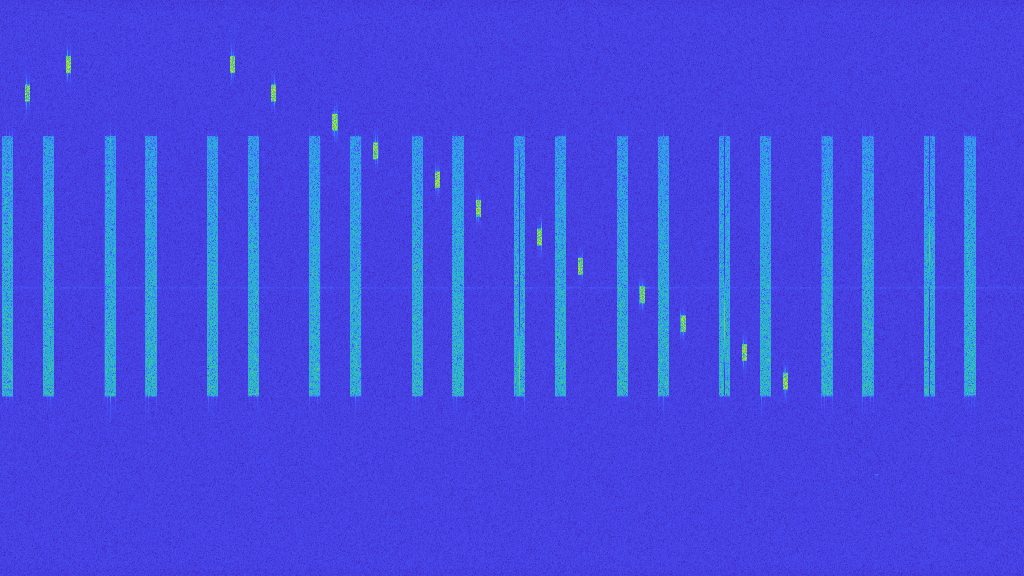
\includegraphics[width=0.90\textwidth]{figuras/introduccion/mini3_drone_d5_w1_s01_cap01__seg0028.png}
    \caption{Ejemplo de espectrograma obtenido a partir de una captura RF del DJI Mini 3 en la banda de \SI{2.4}{\giga\hertz}. Se observan ráfagas estrechas y de corta duración distribuidas en frecuencia, correspondientes a la firma tiempo-frecuencia característica del enlace de comunicaciones del dron. Las bandas más anchas y prolongadas en el tiempo se corresponden con el enlace de descarga de vídeo (\emph{downlink}) del dron, mientras que las ráfagas más estrechas se asocian al canal de control.}
    \label{fig:espectrograma_mini3}
\end{figure}

La formulación inicial del trabajo planteaba una clasificación binaria de espectrogramas completos mediante una red convolucional ResNet18. Aunque este enfoque permitía construir un primer prototipo, el análisis experimental mostró una limitación importante: un clasificador global puede aprender correlaciones espurias del contexto de captura, como diferencias entre escenarios interiores y exteriores, en lugar de centrarse en la firma RF local del dron. Para evitar este problema, el trabajo se reconvierte hacia un detector de objetos basado en YOLOv8 que opera sobre regiones del espectrograma. De este modo, el modelo debe localizar y clasificar ráfagas individuales, reduciendo la dependencia del fondo global de la imagen.

Este cambio conecta el trabajo con arquitecturas recientes de detección e identificación RF en dos etapas, donde una primera red detecta regiones de señal en el espectrograma y una segunda red clasifica el tipo de dron a partir de las regiones detectadas \cite{rfuav2025}. En este TFG, la primera etapa se centra en separar ráfagas asociadas al DJI Mini 3 frente a interferencias WiFi/Bluetooth, y la segunda etapa identifica el modelo concreto de dron a partir de esas regiones, una vez confirmada la presencia de señal.

\section{Planteamiento del problema}
\label{sec:planteamiento}

El problema principal abordado se formula como una tarea de detección de objetos sobre espectrogramas RF. Dada una ventana temporal de señal capturada mediante un receptor SDR, se desea localizar las regiones del espectrograma que contienen ráfagas de señal y clasificarlas como \emph{drone} o \emph{interference}. La clase \emph{drone} representa ráfagas compatibles con la firma OcuSync del DJI Mini 3, mientras que la clase \emph{interference} agrupa ráfagas y estructuras producidas por fuentes no dron, principalmente Bluetooth FHSS, WiFi residual y ruido que supera el umbral de etiquetado.

La dificultad reside en que la banda analizada está compartida por múltiples tecnologías inalámbricas. Una simple medida de potencia recibida no resulta suficiente, ya que una red WiFi cercana puede generar niveles de energía elevados y producir falsas alarmas si el sistema se basa únicamente en umbrales. Además, algunas señales interferentes, como Bluetooth, presentan ráfagas estrechas y saltos en frecuencia que pueden asemejarse parcialmente a la firma del enlace del dron. Por este motivo, el detector se plantea sobre espectrogramas, donde se conserva la evolución temporal y frecuencial de la señal.

La hipótesis de trabajo es que la firma FHSS/OcuSync del DJI Mini 3 deja una huella tiempo-frecuencia diferenciable respecto a otras transmisiones presentes en el entorno, y que un detector de objetos puede aprender dicha huella a partir de cajas generadas sobre las regiones activas del espectrograma. A diferencia de la clasificación de imagen completa, la detección de objetos obliga al modelo a operar sobre regiones locales y permite obtener una salida más interpretable: no solo indica si hay dron, sino también dónde aparece la evidencia dentro de la representación tiempo-frecuencia.

Este planteamiento en dos etapas admite una lectura orientada a producto. La primera etapa actúa como un filtro que permite descartar, a modo de lista blanca, las emisiones no relevantes de la banda —WiFi, Bluetooth y ruido residual—, de modo que el sistema solo retiene las regiones compatibles con un enlace de dron. La segunda etapa opera sobre esas regiones ya filtradas y se orienta a la identificación entre diferentes modelos de dron. Esta tarea plantea una dificultad adicional, ya que no basta con distinguir la presencia de una señal compatible con un UAV frente a interferencias, sino que es necesario identificar diferencias más sutiles entre las firmas RF de distintos enlaces de comunicación. Por ello, dicha clasificación se aplica preferentemente sobre las regiones ya detectadas como señal de dron, y no sobre el espectrograma completo.

De forma complementaria, el trabajo evalúa la robustez del sistema frente a la congestión de la banda y frente al ruido, así como su capacidad de generalizar a otros modelos de dron no vistos durante el entrenamiento. El efecto de la distancia entre dron y receptor se contempla únicamente como variable experimental de las capturas ---a 5 y 10 metros---, sin abordarse como un estudio sistemático ni como un problema de localización métrica; su análisis en profundidad se deja como línea futura.

\section{Objetivos}
\label{sec:objetivos}

\subsection{Objetivo general}

El objetivo principal de este Trabajo Fin de Grado es diseñar, implementar y evaluar un sistema de detección de señales de dron mediante radiofrecuencia, utilizando capturas SDR, espectrogramas tiempo-frecuencia y redes neuronales profundas. El sistema se reformula como una arquitectura en dos etapas: una primera etapa de detección/localización de ráfagas mediante YOLOv8 para distinguir \emph{drone} frente a \emph{interference}, y una segunda etapa de identificación de modelos de dron a partir de señales ya detectadas como compatibles con UAV.

\subsection{Objetivos específicos}

\begin{description}
  \item[OE1] Revisar el estado del arte en detección de drones por radiofrecuencia, prestando especial atención a las técnicas basadas en espectrogramas, detección de objetos y arquitecturas en dos etapas.
  \item[OE2] Definir la metodología de adquisición de señales IQ con SDR en la banda de \SI{2.4}{\giga\hertz} (dron activo e interferencias WiFi/Bluetooth bajo condiciones controladas) y construir un conjunto de datos reproducible a partir de capturas SigMF: segmentación en ventanas de \SI{0.1}{\second}, generación de espectrogramas y auto-etiquetado de cajas delimitadoras mediante umbrales de energía y filtros morfológicos.
  \item[OE3] Entrenar y evaluar un detector YOLOv8 que localice y clasifique las ráfagas como \emph{drone} o \emph{interference}, utilizando métricas propias de detección (precisión, recall, mAP@50 y mAP@50-95), y compararlo con el enfoque previo de clasificación global para justificar la reducción del sesgo contextual.
  \item[OE4] Analizar la robustez del sistema frente a la congestión de la banda (WiFi y Bluetooth) y frente al ruido, verificando si la discriminación aprendida se sustenta en la morfología espectro-temporal de las ráfagas o en el nivel medio de potencia.
  \item[OE5] Desarrollar y evaluar una segunda etapa de identificación entre modelos de dron, basada en redes convolucionales como ResNet18, aplicada sobre las regiones o espectrogramas filtrados por la etapa de detección, y comprobar su capacidad de generalización a drones no vistos en el entrenamiento.
\end{description}

\section{Alcance del trabajo}
\label{sec:alcance}

El alcance principal del TFG queda delimitado a la detección de actividad de dron frente a interferencias en espectrogramas RF de la banda de \SI{2.4}{\giga\hertz}. El sistema se valida con capturas reales del DJI Mini 3 y escenarios sin dron con presencia de WiFi/Bluetooth. La contribución central no es decodificar protocolos propietarios ni estimar la posición exacta del dron, sino evaluar si la morfología tiempo-frecuencia de las ráfagas permite distinguir señal de dron frente a interferencias mediante aprendizaje profundo.

El trabajo incluye la adquisición de señales IQ, su almacenamiento en formato SigMF, la generación de espectrogramas, el auto-etiquetado de regiones activas, el entrenamiento de un detector YOLOv8 y la evaluación del modelo con métricas de detección. La identificación de modelos de drones constituye la segunda etapa del sistema, aplicada sobre las regiones filtradas por la detección inicial. La distancia entre dron y receptor se contempla solo como variable experimental de las capturas, no como un sistema de localización ni como un estudio sistemático de su efecto.

Cabe plantearse si este problema podría resolverse analizando directamente los paquetes de datos transmitidos en la banda ISM, en lugar de su morfología tiempo-frecuencia. Sin embargo, este enfoque no es viable en el caso general: los enlaces de comunicación de los drones comerciales, como OcuSync de DJI, emplean protocolos propietarios y cifrado de la información, por lo que el contenido de los paquetes no resulta accesible ni decodificable por un receptor pasivo. El análisis basado en la firma RF —la morfología de las ráfagas FHSS en el espectrograma— es independiente del cifrado, ya que opera sobre características físicas de la transmisión (duración, ancho de banda y patrón de salto en frecuencia) que permanecen observables aunque la carga útil esté encriptada. Por ello, la detección a nivel de señal resulta más robusta y general que cualquier intento de inspección de paquetes.

\section{Presupuesto y planificación}
\label{sec:presupuesto_planificacion}

\subsection{Recursos materiales y presupuesto}

El desarrollo del trabajo requiere un receptor SDR compatible con la banda de \SI{2.4}{\giga\hertz}, antenas adecuadas, un ordenador con GPU para adquisición y entrenamiento, el dron empleado como fuente de señal y software de procesado y aprendizaje profundo. En la parte de adquisición se emplea GNU Radio junto con un USRP B210 o dispositivo equivalente. En la parte de entrenamiento se utiliza Python con bibliotecas científicas y de aprendizaje profundo, incluyendo PyTorch y Ultralytics YOLO. Todo el software empleado es de código abierto o de uso académico gratuito, por lo que su coste de licencia es nulo.

El presupuesto se estima diferenciando entre el coste del material y el coste de personal. La \cref{tab:presupuesto_material} resume el coste de material y la \cref{tab:presupuesto_total} el presupuesto total.

\begin{table}[htbp]
\centering
\caption{Coste de material del proyecto.}
\label{tab:presupuesto_material}
\begin{tabular}{lc}
\toprule
\textbf{Concepto} & \textbf{Coste (EUR)} \\
\midrule
Receptor SDR USRP B210 & 1200 \\
Portátil con GPU (RTX 4070) & 1600 \\
Dron DJI Mini 3 & 510 \\
Antena directional 2,4~GHz & 80 \\
Cableado y adaptadores SMA & 30 \\
Software (GNU Radio, Python, PyTorch, Ultralytics) & 0 \\
\midrule
\textbf{Subtotal material} & \textbf{3420} \\
\bottomrule
\end{tabular}
\end{table}

El coste de personal se estima a partir de las horas de dedicación recogidas en la planificación. Para el ingeniero junior se considera el coste bruto para la empresa, que incluye no solo el salario bruto del trabajador (en torno a \SI{18}{EUR/h}) sino también los costes de contratación a cargo del empleador (cotizaciones a la Seguridad Social, etc.), que suponen aproximadamente un \SI{55}{\percent} adicional, resultando en un coste efectivo de unos \SI{27.9}{EUR/h}. La \cref{tab:presupuesto_total} reúne el coste de personal, el de material y el presupuesto total del proyecto.

\begin{table}[htbp]
\centering
\caption{Presupuesto total del proyecto (material y personal).}
\label{tab:presupuesto_total}
\begin{tabular}{lc}
\toprule
\textbf{Concepto} & \textbf{Coste (EUR)} \\
\midrule
Personal: ingeniero junior (350~h $\times$ 27,9~EUR/h) & 9765 \\
Personal: tutorización (25~h $\times$ 45~EUR/h) & 1125 \\
\textbf{Subtotal personal} & \textbf{10890} \\
\midrule
Subtotal material (\cref{tab:presupuesto_material}) & 3420 \\
\midrule
\textbf{Total} & \textbf{14310} \\
\bottomrule
\end{tabular}
\end{table}




El trabajo se organiza en cinco fases principales, parcialmente solapadas: revisión bibliográfica, adquisición y organización de capturas, generación del dataset de espectrogramas, entrenamiento y evaluación del detector YOLO, y redacción de la memoria. La segunda etapa de identificación de modelos se desarrolla con posterioridad, una vez validado que la primera etapa permite separar señal de dron e interferencias. La \cref{tab:planificacion} recoge la duración aproximada de cada fase.

\begin{table}[htbp]
\centering
\caption{Planificación temporal aproximada del trabajo.}
\label{tab:planificacion}
\begin{tabularx}{\textwidth}{lcX}
\toprule
\textbf{Fase} & \textbf{Duración aprox.} & \textbf{Actividades principales} \\
\midrule
F1. Revisión bibliográfica & 3 semanas & Estado del arte en detección RF de drones, espectrogramas y detección de objetos. \\
F2. Adquisición de capturas & 4 semanas & Montaje SDR, metodología de captura, sesiones de dron e interferencia. \\
F3. Generación del dataset & 3 semanas & STFT, espectrogramas, auto-etiquetado y particiones por captura. \\
F4. Entrenamiento y evaluación & 5 semanas & Entrenamiento YOLOv8n, métricas, matriz de confusión y análisis. \\
F5. Redacción de la memoria & 6 semanas & Redacción, figuras, revisión y correcciones. \\
\bottomrule
\end{tabularx}
\end{table}

\section{Estructura del documento}
\label{sec:estructura}

El documento se organiza de la siguiente forma. El \cref{cap:introduccion} presenta la motivación, el problema y los objetivos del trabajo. El \cref{cap:estado_arte} revisa las principales tecnologías de detección de drones, las características de las señales RF y el uso de espectrogramas con aprendizaje profundo. El \cref{cap:requisitos_diseno} define los requisitos y el diseño del sistema, incluyendo la arquitectura en dos etapas. El \cref{cap:implementacion} describe la adquisición de señal, la generación de espectrogramas, el auto-etiquetado de ráfagas y el entrenamiento de YOLO. El \cref{cap:pruebas_resultados} presenta el protocolo experimental, las métricas y los resultados obtenidos. Finalmente, el \cref{cap:conclusiones} resume las conclusiones, limitaciones y líneas futuras.

% =============================================================================
% Capitulo 2 - Estado del arte
% =============================================================================
\chapter{Estado del arte}
\label{cap:estado_arte}

\section{Sistemas de detección de drones}
\label{sec:deteccion_drones}

La proliferación de drones comerciales de bajo coste ha provocado un crecimiento sostenido de incidentes en infraestructuras críticas durante la última década. El cierre del aeropuerto londinense de Gatwick en diciembre de 2018, la invasión del espacio aéreo de plantas nucleares francesas en 2019 o las múltiples incursiones detectadas sobre instalaciones militares europeas han convertido el llamado \emph{counter-UAS}  en un dominio tecnológico con producto comercial maduro y literatura académica abundante \cite{taha2022counteruav,shi2025airport}. Este capítulo revisa las principales familias tecnológicas empleadas para detectar drones, los sistemas comerciales más representativos de cada una y justifica la elección de la aproximación basada en radiofrecuencia adoptada en este TFG.

\subsection{Familias tecnológicas}
\label{subsec:familias_deteccion}

La detección de un dron se aborda habitualmente con cuatro tipos de sensores que explotan principios físicos distintos.

\textbf{Radar.} Los sistemas radar iluminan activamente el espacio con ondas electromagnéticas y analizan los ecos reflejados por el blanco. Son la solución tradicional en vigilancia aérea, pero los drones de pequeño tamaño  presentan una sección radar (RCS) muy reducida, lo que ha obligado a desarrollar radares específicos en banda K o Ka con escaneo electrónico. Funcionan en cualquier condición de iluminación y meteorología, pero son sistemas activos que emiten energía, requieren licencia y resultan costosos \cite{taha2022counteruav}.

\textbf{Acústica.} Los sensores acústicos detectan el ruido característico de los motores y hélices del dron mediante arrays de micrófonos y técnicas de \emph{beamforming}. Son pasivos, baratos y operan en condiciones de baja visibilidad, pero su alcance está fuertemente limitado por la atenuación del sonido en el aire y por el ruido de fondo urbano. Funcionan bien para clases pequeñas a corta distancia  y se han convertido en un componente recurrente de redes de bajo coste, como las desplegadas durante el conflicto de la guerra de Ucrania.

\textbf{Óptica.} Las cámaras visibles e infrarrojas confirman visualmente la presencia del dron y permiten su identificación. Son imprescindibles como capa de verificación final, pero por sí solas presentan limitaciones importantes: dependencia de iluminación, vulnerabilidad a la meteorología adversa, campos de visión estrechos y necesidad de saber dónde apuntar. En la práctica, se utilizan en arquitecturas \emph{slew-to-cue} guiadas por otro sensor primario \cite{shi2025airport}.

\textbf{Radiofrecuencia.} Los sistemas RF capturan de forma pasiva las comunicaciones entre el dron y su mando, o entre el dron y el satélite GNSS, y las clasifican por su firma espectral. Aprovechan que la mayoría de drones comerciales mantienen un enlace de mando, telemetría o vídeo activo durante toda la operación. Son completamente pasivos, no requieren licencia de emisión, y permiten detectar el dron incluso antes de que esté en línea de vista directa (NLOS), ya que la radio del piloto y la del dron son detectables por separado. Su limitación más conocida es la incapacidad para detectar drones controlados por fibra óptica o autónomos sin enlace, situación que ha cobrado relevancia operacional reciente \cite{taha2022counteruav}.

\subsection{Sistemas comerciales destacados}
\label{subsec:sistemas_comerciales}

Como referencia del estado de la técnica industrial, se describen brevemente los productos más representativos en cada familia tecnológica. La selección se ha realizado priorizando sistemas con documentación técnica pública y referencias en la literatura académica de \emph{counter-UAS}.

\textbf{DroneShield RfOne MKII.} Sensor estacionario de detección y radiogoniometría RF completamente pasivo, con cobertura de \ang{90} por unidad y capacidad de combinar cuatro sensores para alcanzar cobertura \ang{360}. Opera contra una base de datos propietaria de firmas RF actualizada por suscripción y permite triangulación cuando se despliegan varios sensores en red \cite{droneshield_rfone}.


\begin{figure}[H]
    \centering
    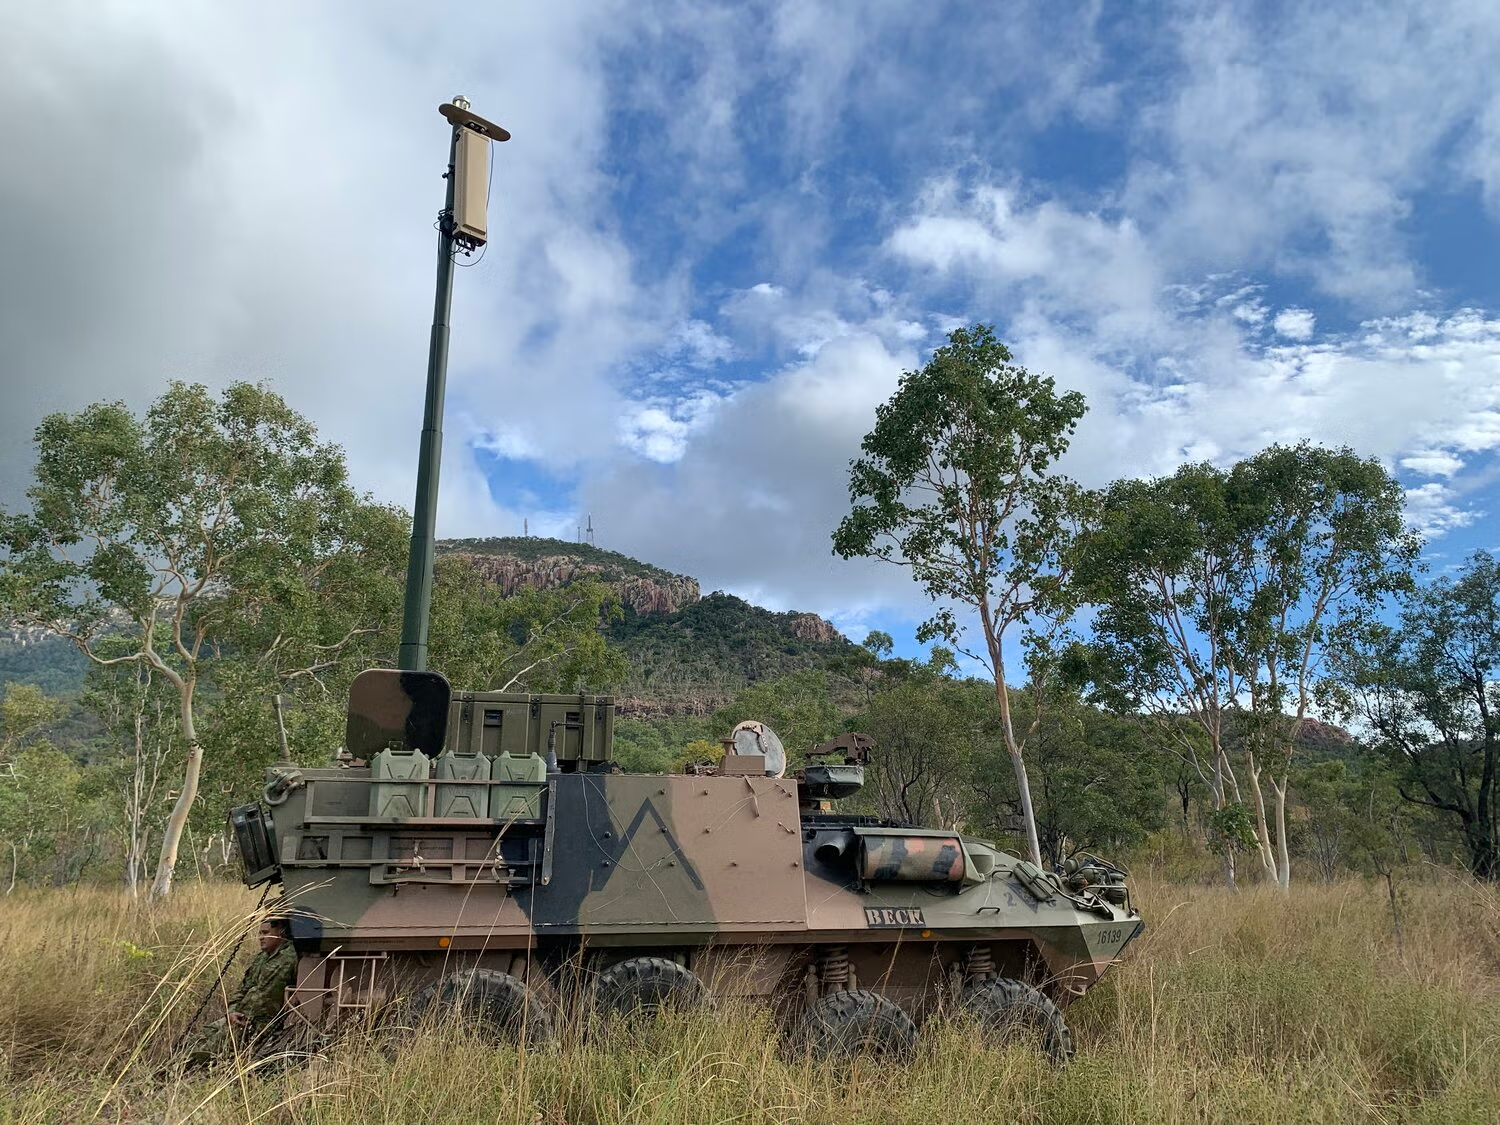
\includegraphics[width=0.6\textwidth]{figuras/estado del arte/Army2-6.png}
    \caption{Sensor estacionario de detección y radiogoniometría RF DroneShield RfOne MKII, desplegado para vigilancia de largo alcance. Fuente: DroneShield~\cite{droneshield_rfone}.}
    \label{fig:droneshield_rfone}
\end{figure}

\textbf{Aaronia AARTOS.} Plataforma modular construida en torno al analizador de espectro en tiempo real SPECTRAN V6, que ofrece hasta \SI{980}{\mega\hertz} de ancho de banda instantáneo en el rango \SIrange{10}{8000}{\mega\hertz}. Combinado con la antena IsoLOG 3D DF y la suite RTSA-Suite PRO, decodifica protocolos como DJI OcuSync y Mavlink y alcanza hasta \SI{50}{\kilo\meter} de rango de detección en configuraciones desplegadas \cite{aaronia_aartos}.

\begin{figure}[H]
    \centering
    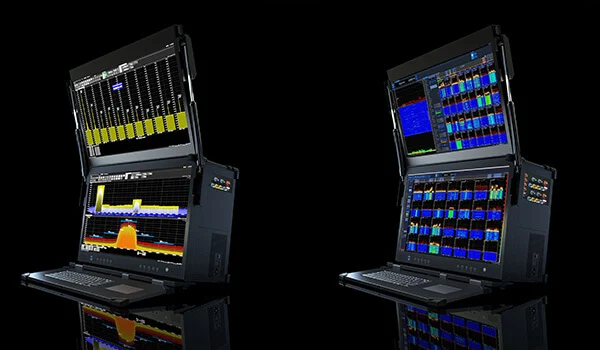
\includegraphics[width=0.6\textwidth]{figuras/estado del arte/aaronia.png}
    \caption{Sistema de detección de drones Aaronia AARTOS, construido en torno al analizador de espectro en tiempo real SPECTRAN V6 y la antena IsoLOG 3D DF. Fuente: Aaronia AG~\cite{aaronia_aartos}.}
    \label{fig:aaronia_aartos}
\end{figure}

\textbf{Dedrone RF-360.} Sensor RF pasivo en red, con grado de protección IP65 y conectividad LTE/GPS integrada para despliegue rápido. Integra varios SDR internos que clasifican el dron mediante la suite DroneTracker y permite localización por triangulación con alcance de hasta \SI{5}{\kilo\meter} en configuraciones direccionales \cite{dedrone_rf360}.


\begin{figure}[H]
    \centering
    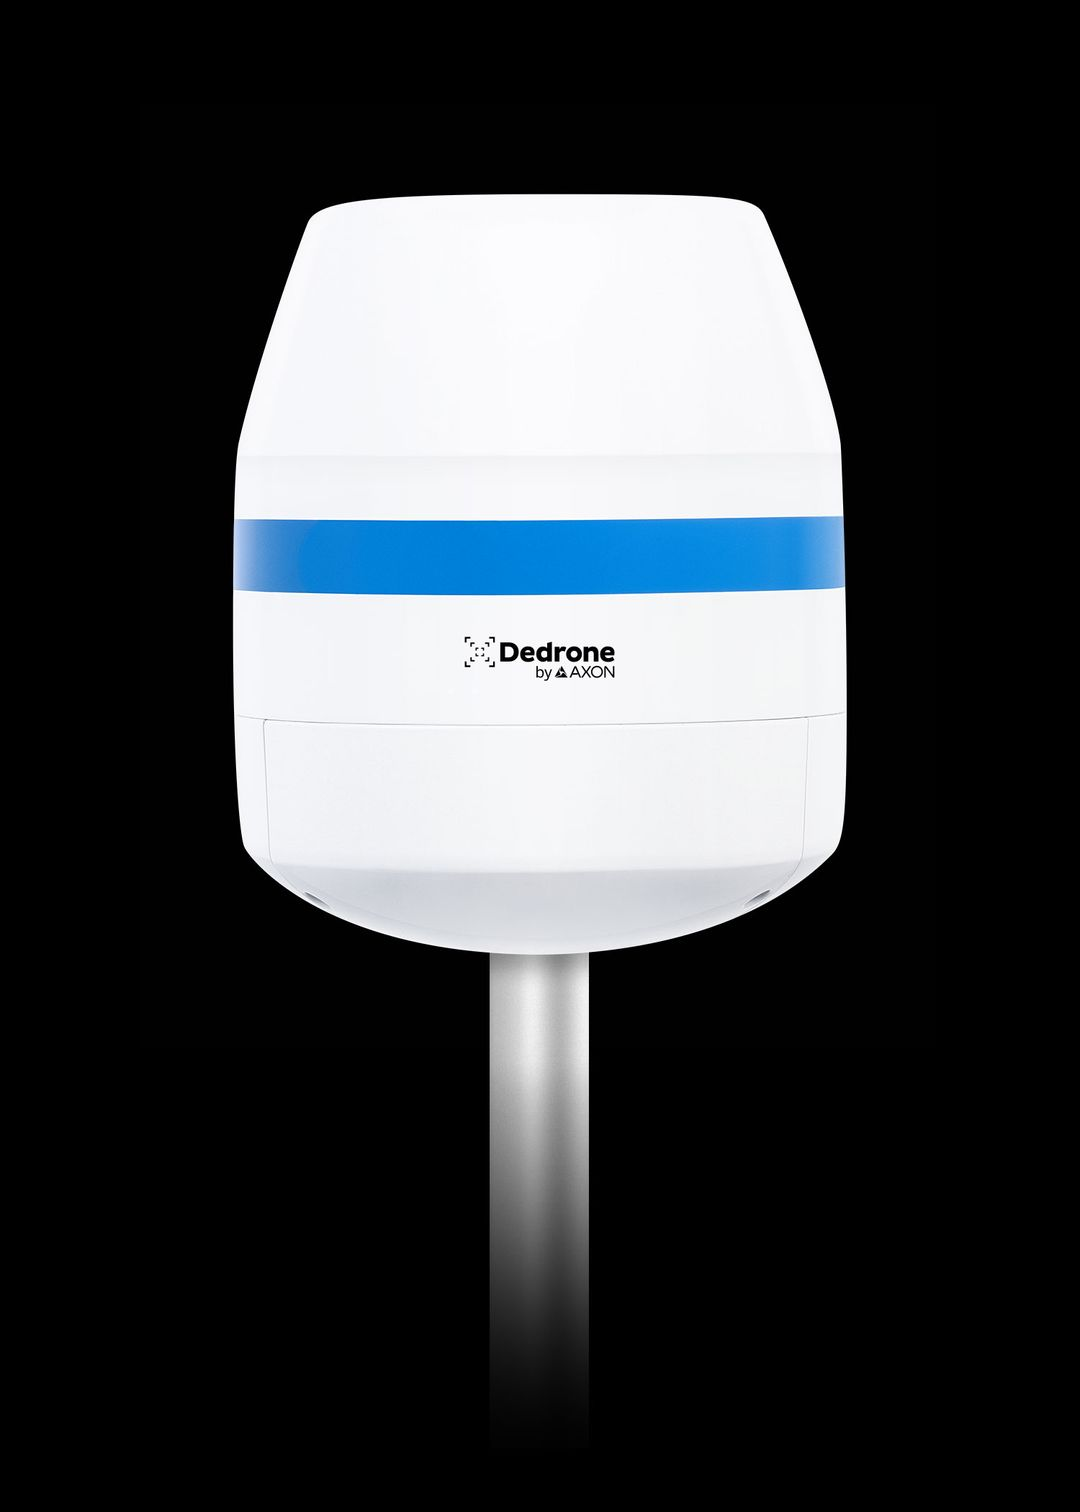
\includegraphics[width=0.6\textwidth]{figuras/estado del arte/dedrone.jpg}
    \caption{Sensor RF pasivo en red Dedrone RF-360, con grado de protección IP65 y conectividad LTE/GPS integrada para despliegue rápido. Fuente: Dedrone~\cite{dedrone_rf360}.}
    \label{fig:dedrone_rf360}
\end{figure}

\textbf{Rohde \& Schwarz ARDRONIS.} Sistema profesional de detección, clasificación y localización RF que cubre \SIrange{20}{6000}{\mega\hertz} con una única antena. Su característica más relevante para este TFG es el algoritmo de separación automática basada en perfiles, capaz de aislar la señal de un enlace FHSS concreto en escenarios con espectro densamente ocupado \cite{rohde_ardronis}.

\begin{figure}[H]
    \centering
    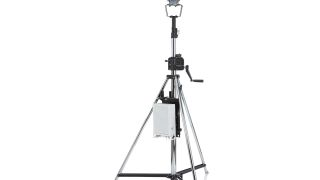
\includegraphics[width=0.6\textwidth]{figuras/estado del arte/ardronis.jpg}
    \caption{Sistema de detección, clasificación y localización RF Rohde \& Schwarz ARDRONIS, con algoritmo de separación automática de enlaces FHSS en espectro densamente ocupado. Fuente: Rohde \& Schwarz~\cite{rohde_ardronis}.}
    \label{fig:rohde_ardronis}
\end{figure}

\subsection{Comparativa y justificación de la elección RF}




La aproximación RF resulta especialmente adecuada para un TFG experimental por tres razones. En primer lugar, la captura es pasiva y se realiza con receptores SDR de coste moderado (HackRF, USRP, BladeRF), lo que evita los problemas regulatorios asociados a sensores activos. En segundo lugar, los drones comerciales mayoritarios mantienen su enlace de mando activo en bandas ISM bien delimitadas (\SI{2.4}{\giga\hertz} y \SI{5.8}{\giga\hertz}), lo que permite trabajar sobre datasets reproducibles y dispositivos accesibles como el DJI Mini 3. En tercer lugar, la representación tiempo-frecuencia de la señal RF habilita el uso de arquitecturas estándar de visión por computador, conectando el problema con un campo metodológicamente maduro \cite{rfuav2025,allahham2019dronerf}.

El principal riesgo de la aproximación RF es la presencia simultánea de WiFi y Bluetooth en la banda de \SI{2.4}{\giga\hertz}, que comparten morfología FHSS y OFDM con el enlace del dron y constituyen el reto técnico que motiva este trabajo. Las secciones siguientes profundizan en la caracterización RF del enlace del DJI Mini 3 (Sección~\ref{sec:comunicaciones_rf}), las representaciones tiempo-frecuencia empleadas (Sección~\ref{sec:representaciones_tf}) y los modelos de aprendizaje profundo aplicables al problema (Sección~\ref{sec:deep_rf}).


\section{Comunicaciones RF en drones comerciales}
\label{sec:comunicaciones_rf}

Para entender la dificultad de la detección RF de drones es necesario conocer qué señales conviven en la banda en la que estos operan y qué morfología presentan en un espectrograma. Esta sección describe brevemente el contexto de la banda \SI{2.4}{\giga\hertz}, los enlaces de control y vídeo más extendidos en drones comerciales, y las clases de señal que actúan habitualmente como interferencia.

\subsection{La banda ISM de 2,4~GHz}
\label{subsec:banda_ism}

La banda \emph{Industrial, Scientific and Medical} (ISM) de \SIrange{2400}{2483.5}{\mega\hertz} está disponible sin licencia en prácticamente todo el mundo. Como consecuencia, es compartida por una gran variedad de tecnologías inalámbricas, entre ellas WiFi (802.11\,b/g/n/ax), Bluetooth Classic y Bluetooth Low Energy, ZigBee, hornos microondas, sistemas de mando radioeléctrico para modelismo y la mayoría de enlaces de control de drones comerciales \cite{ieee80211_2020,bluetooth_core_5_4}. Esta coexistencia obliga a cualquier detector basado en RF a operar en un entorno crónicamente congestionado, donde la mera presencia de energía en la banda no es informativa.

WiFi ocupa canales de \SI{20}{\mega\hertz} (con bonding opcional a \SI{40}{\mega\hertz}) centrados a partir de \SI{2412}{\mega\hertz} con separación de \SI{5}{\mega\hertz}, lo que da hasta catorce canales solapados de los que solo tres (1, 6 y 11) son habitualmente utilizables sin colisión. Bluetooth Classic divide la banda en \num{79} canales de \SI{1}{\mega\hertz} y salta entre ellos a una tasa de \num{1600} saltos por segundo siguiendo una secuencia pseudoaleatoria.







\subsection{La plataforma DJI Mini 3 y el enlace OcuSync O2}
\label{sec:plataforma_mini3}

El dron empleado como fuente de señal en este trabajo es el DJI Mini 3. Su enlace de comunicación con el mando utiliza el sistema de transmisión de vídeo \emph{OcuSync O2} (comercializado por DJI como \emph{DJI O2}), el mismo que monta el DJI Mini 2; la variante DJI Mini 3 Pro emplea, en cambio, la generación posterior OcuSync O3~\cite{dji_mini3_manual,heliguy_dji_transmission}. El enlace opera en las bandas de \SIrange{2.4000}{2.4835}{\giga\hertz} y \SIrange{5.725}{5.850}{\giga\hertz}. Este trabajo se centra en la banda de \SI{2.4}{\giga\hertz}, donde el enlace coexiste con WiFi y Bluetooth.

La característica más relevante para la detección es que OcuSync emplea salto de frecuencia (FHSS) con selección adaptativa del canal: el sistema es capaz de elegir automáticamente el mejor canal de transmisión, evitando las zonas del espectro más congestionadas por otras señales. En la práctica, esto significa que las ráfagas del enlace tienden a situarse en los huecos libres entre los canales WiFi ocupados (típicamente los canales 1, 6 y 11), de forma análoga al salto de frecuencia adaptativo (AFH) del Bluetooth. Como consecuencia, en un espectrograma de la banda las transmisiones del dron aparecen como ráfagas estrechas y dispersas en frecuencia, en lugar de columnas anchas y fijas como las del WiFi.

Este comportamiento es lo que hace interesante el problema: la firma del dron no ocupa una posición fija del espectro, sino que se reparte dinámicamente por los huecos libres, compartiendo banda y morfología con otras señales de salto de frecuencia como el Bluetooth. Conviene además señalar que el propio DJI Mini 3 integra módulos WiFi y Bluetooth 5.2.








\subsection{Enlaces de control y vídeo de drones comerciales}
\label{subsec:enlaces_drones}

Los drones comerciales suelen mantener dos canales de comunicación activos durante el vuelo: un enlace de mando y telemetría hacia el dron, y un enlace de vídeo descendente. El sistema más extendido en el mercado de consumo es la familia OcuSync de DJI, que ha evolucionado desde Lightbridge (2014) hasta las generaciones actuales O3 y O4 \cite{heliguy_dji_transmission}. Todas las versiones de OcuSync emplean modulación OFDM para el vídeo y un mecanismo de salto en frecuencia (FHSS) para el mando, con anchos de banda configurables y operación dual en \SI{2.4}{\giga\hertz} y \SI{5.8}{\giga\hertz} \cite{schiller2023droneid}. Además, los drones DJI modernos emiten paquetes \emph{DroneID} para cumplir con normativas Remote-ID, con una estructura periódica de ráfagas cortas en el orden de centenares de microsegundos y anchos de banda de pocos megahercios \cite{schiller2023droneid,vainilavicius2024dji}.

Fuera del ecosistema DJI conviven otros sistemas RC abiertos. ExpressLRS (ELRS) es un protocolo de código abierto basado en transceptores Semtech (LoRa y FLRC) que opera en \SI{2.4}{\giga\hertz} y \num{868}/\SI{915}{\mega\hertz} \cite{expresslrs}. TBS Crossfire combina DSSS y FHSS en bandas sub-GHz \cite{tbs_crossfire}. Por último, los drones de bajo coste basados en WiFi-FPV (Parrot AR.Drone y similares) producen una firma indistinguible de una red WiFi convencional. Para el propósito de este TFG resulta especialmente relevante OcuSync, por ser el sistema utilizado en la mayoría de drones de consumo actuales.






\subsection{Comparativa morfológica de las señales en 2,4~GHz}
\label{subsec:comparativa_morfologia}

Desde el punto de vista de un espectrograma, las tres clases de señal más significativas en la banda presentan estructuras visualmente distinguibles. WiFi se manifiesta como columnas verticales anchas y persistentes coincidentes con los canales fijos. El enlace OFDM de vídeo de los drones aparece como una banda continua de anchura media. Bluetooth Classic y el enlace de mando FHSS de OcuSync producen ráfagas estrechas y dispersas, geométricamente similares entre sí, lo que constituye el principal reto del problema. La Figura~\ref{fig:espectrograma_interferencia} ilustra estas estructuras en una captura sin presencia de dron, y la Tabla~\ref{tab:morfologia_rf} resume las propiedades morfológicas de cada clase.

\begin{figure}[H]
\centering
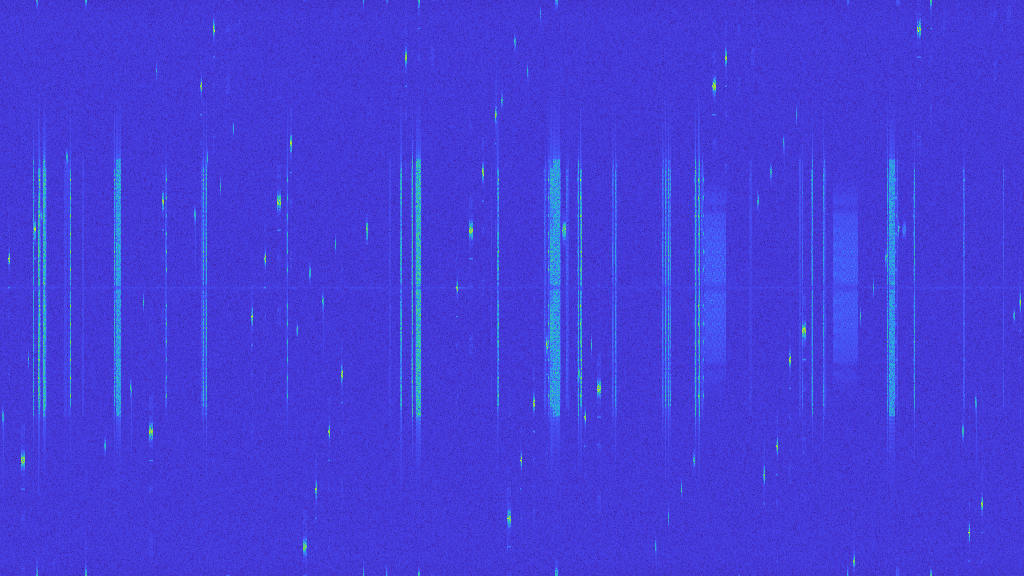
\includegraphics[width=0.95\textwidth]{figuras/estado del arte/mini3_nodrone_w2_s01_cap03__seg0068.png}
\caption{Ejemplo de espectrograma en la banda de \SI{2.4}{\giga\hertz} con interferencia WiFi y Bluetooth. Las columnas verticales anchas corresponden a canales WiFi ocupados; las ráfagas estrechas y dispersas son atribuibles a Bluetooth y a otros emisores ISM, y presentan una morfología parcialmente similar a la firma esperada del enlace de mando de un dron.}
\label{fig:espectrograma_interferencia}
\end{figure}

\begin{table}[H]
\centering
\caption{Comparativa morfológica de las señales presentes en la banda de \SI{2.4}{\giga\hertz}.}
\label{tab:morfologia_rf}
\begin{tabularx}{\textwidth}{lXXXX}
\toprule
\textbf{Propiedad} & \textbf{OcuSync (mando)} & \textbf{OcuSync (vídeo)} & \textbf{WiFi 802.11g/n} & \textbf{Bluetooth Classic} \\
\midrule
Técnica & FHSS & OFDM adaptativo & OFDM en canal fijo & FHSS \\
Ancho de banda & Estrecho por ráfaga & Medio/ancho continuo & Ancho, canal fijo & Muy estrecho por salto \\
Duración de actividad & Ráfagas cortas dispersas & Continua durante vídeo & Por tramas, ráfagas variables & Ráfagas muy cortas, periódicas \\
Posición en frecuencia & Variable & Centrada en canal libre & Canales fijos (1, 6, 11) & Distribuida por toda la banda \\
Apariencia espectral & Rectángulos pequeños dispersos & Banda continua bien definida & Columnas verticales anchas & Rectángulos pequeños dispersos \\
\bottomrule
\end{tabularx}
\end{table}

La similitud morfológica entre las ráfagas FHSS de Bluetooth y las del enlace de mando del dron es el motivo por el que la detección no puede basarse en simples descriptores espectrales agregados y motiva el uso de modelos de aprendizaje profundo capaces de aprender patrones tiempo-frecuencia más sutiles, como los descritos en las secciones siguientes.

\section{Representaciones tiempo-frecuencia de señales RF}
\label{sec:representaciones_tf}

La clasificación de señales de radiofrecuencia mediante aprendizaje profundo requiere transformar las muestras IQ del receptor en una representación bidimensional que la red pueda procesar como una imagen. La literatura ha explorado varias alternativas, todas ellas basadas en mostrar simultáneamente cómo se distribuye la energía de la señal en tiempo y en frecuencia \cite{cohen1995timefrequency,boashash2015timefrequency}.

El espectrograma derivado de la transformada de Fourier de tiempo corto (STFT) es la representación más extendida. Trabajos recientes sobre clasificación de drones por RF, como RFUAV \cite{rfuav2025} o DroneRF \cite{allahham2019dronerf}, lo emplean como entrada estándar a arquitecturas convolucionales preentrenadas, aprovechando que su formato matricial encaja directamente con redes diseñadas para imágenes naturales. Su popularidad se explica por tres factores: un coste computacional reducido, una buena estabilidad numérica y la compatibilidad inmediata con modelos como ResNet, VGG o EfficientNet sin necesidad de adaptaciones.

Otras representaciones aparecen ocasionalmente en la literatura. El escalograma, obtenido mediante la transformada wavelet continua (CWT), ofrece resolución adaptativa y resulta atractivo para señales con eventos transitorios de muy distintas duraciones \cite{mallat2008wavelet}. Las distribuciones cuadráticas como la de Wigner-Ville proporcionan una resolución conjunta tiempo-frecuencia superior a la STFT, pero introducen términos cruzados que dificultan su interpretación visual y su uso con redes convolucionales \cite{boashash2015timefrequency}. En el ámbito específico de la detección y clasificación RF de drones mediante aprendizaje profundo, el espectrograma STFT se ha consolidado como la representación de referencia.




\section{Aprendizaje profundo para detección y clasificación de señales RF}
\label{sec:deep_rf}

Las redes neuronales convolucionales han demostrado gran capacidad para extraer patrones espaciales en imágenes. Al convertir una señal RF en un espectrograma, la tarea puede tratarse como un problema de reconocimiento de patrones visuales, donde las estructuras relevantes son ráfagas, bandas, discontinuidades, densidad de ocupación o cambios de energía. Dentro de este marco, este trabajo emplea dos familias de arquitecturas con propósitos distintos: una red de clasificación de imágenes (ResNet) y una red de detección de objetos (YOLO).

\subsection{Redes convolucionales residuales: ResNet}
\label{subsec:resnet}

ResNet (\emph{Residual Network}) es una arquitectura convolucional introducida por He et~al. \cite{he2016resnet} que resolvió el problema de degradación que aparece al aumentar la profundidad de las redes. Su aportación clave son las \emph{conexiones residuales} o de salto, que suman la entrada de un bloque a su salida y permiten que el gradiente fluya directamente a través de la red. Gracias a ello es posible entrenar modelos de decenas o cientos de capas sin que el entrenamiento se degrade. La familia incluye variantes de distinta profundidad (ResNet18, 34, 50, 101, 152); la versión ResNet18, con aproximadamente once millones de parámetros, ofrece un buen compromiso entre capacidad y coste computacional.

Una característica determinante para este trabajo es la disponibilidad de pesos preentrenados sobre ImageNet, lo que permite aplicar \emph{transfer learning}: se reutiliza el extractor de características aprendido sobre imágenes naturales y se sustituye únicamente la capa final por una salida adaptada a las clases del problema. Esto reduce drásticamente la cantidad de datos y de tiempo de entrenamiento necesarios, algo especialmente valioso en un dataset RF de tamaño limitado.

En este TFG, ResNet18 se utiliza como clasificador de imagen completa: primero como detector binario \emph{drone}/\emph{interference} en un enfoque inicial, y posteriormente como segunda etapa del sistema, encargada de identificar el modelo concreto de dron a partir de la región o el espectrograma asociado a una detección.

\subsection{Detección de objetos en una etapa: YOLO}
\label{subsec:yolo}

A diferencia de la clasificación, que asigna una única etiqueta a la imagen completa, la \emph{detección de objetos} localiza y clasifica simultáneamente múltiples regiones dentro de la imagen mediante cajas delimitadoras (\emph{bounding boxes}). YOLO (\emph{You Only Look Once}), propuesto por Redmon et~al. \cite{redmon2016yolo}, fue uno de los primeros detectores de una sola etapa: en lugar de proponer regiones candidatas y clasificarlas después (enfoque en dos etapas, como R-CNN), plantea la detección como una única regresión sobre una rejilla que predice cajas y probabilidades de clase en una sola pasada. Esto le confiere una velocidad muy superior, apta para operación en tiempo real.

La versión empleada en este trabajo es YOLOv8, desarrollada por Ultralytics \cite{jocher2023yolov8}. Respecto a versiones anteriores incorpora un diseño \emph{anchor-free} (predice directamente la posición de las cajas sin anclas predefinidas), una cabeza de detección desacoplada y un \emph{backbone} convolucional optimizado, y se distribuye en variantes de distinto tamaño (n, s, m, l, x). La variante \emph{nano} (YOLOv8n), con unos tres millones de parámetros, es la más ligera. El rendimiento de estos detectores se mide habitualmente con la precisión media promedio (mAP) a distintos umbrales de solapamiento (IoU) entre las cajas predichas y las reales.

En este TFG, YOLOv8 constituye la primera etapa del sistema: en lugar de clasificar el espectrograma completo, detecta y localiza las ráfagas individuales dentro de él. Esta decisión es metodológicamente relevante, ya que al operar sobre regiones locales el modelo se ve obligado a atender a la morfología de las ráfagas y no al contexto global de la captura, evitando el sesgo que afectaba al enfoque de clasificación de imagen completa.

\subsection{Sistema en dos etapas y referencia RFUAV}
\label{subsec:two_stage_rfuav}

La combinación de ambas arquitecturas define un sistema en dos etapas: YOLO responde a la pregunta de presencia y localización , mientras que ResNet18 responde a la de identificación. Esta separación permite que cada red resuelva un problema acotado y más sencillo que el problema global.

El trabajo RFUAV constituye la referencia más cercana, ya que propone un conjunto de datos de señales RF de drones y una metodología basada en la conversión de datos IQ a espectrogramas para aplicar después modelos de aprendizaje profundo \cite{rfuav2025}. Este TFG toma esa idea general, pero la adapta a un caso experimental propio centrado en la detección de la firma del dron frente a interferencias WiFi/Bluetooth y en su posterior clasificación por modelos.



\section{Conclusiones del estado del arte}
\label{sec:conclusiones_estado_arte}

La revisión realizada muestra que la detección de drones mediante radiofrecuencia es una línea madura y activa. Las familias tecnológicas disponibles (óptica, acústica, radar y RF) presentan ventajas complementarias, pero los sistemas basados en RF destacan por su carácter pasivo, su capacidad de operar a largo alcance y su compatibilidad con receptores SDR de bajo coste, lo que los convierte en una opción especialmente atractiva para entornos experimentales y académicos.

El análisis de las comunicaciones empleadas por los drones comerciales revela que la banda de \SI{2.4}{\giga\hertz} es un escenario complejo en el que coexisten enlaces propietarios como OcuSync, redes WiFi, dispositivos Bluetooth y otras emisiones ISM. Esta coexistencia obliga a abordar el problema más allá de la simple detección de energía, ya que las firmas relevantes deben distinguirse en presencia de interferencias estructuralmente similares. Las representaciones tiempo-frecuencia, y en particular el espectrograma, se han consolidado en la literatura como entrada estándar para esta tarea, al hacer visibles patrones que en el dominio temporal resultan difíciles de separar.

Sobre esta representación, las arquitecturas de aprendizaje profundo basadas en redes convolucionales han demostrado un rendimiento sólido en problemas de clasificación de señales RF, apoyándose en datasets públicos cada vez más amplios. Sin embargo, gran parte de los trabajos existentes evalúan sus modelos en condiciones controladas o con interferencias limitadas, y un porcentaje reducido incorpora técnicas de interpretabilidad que permitan verificar que la red aprende características físicamente significativas y no artefactos del dataset.

De este recorrido se desprende que el problema sigue abierto en su vertiente más realista: la evaluación de detectores RF basados en aprendizaje profundo frente a escenarios con congestión espectral elevada y la validación, mediante herramientas de interpretabilidad, de que las decisiones del modelo se apoyan en la huella tiempo-frecuencia del enlace del dron. Este es el contexto en el que se enmarca el presente trabajo.
% =============================================================================
% Capitulo 3 - Requisitos y diseño del sistema
% =============================================================================
\chapter{Requisitos y diseño del sistema}
\label{cap:requisitos_diseno}

\section{Requisitos del sistema}
\label{sec:requisitos}

\subsection{Requisitos funcionales}

El sistema propuesto debe cubrir el flujo completo desde la adquisición RF hasta la decisión final del detector. Los requisitos funcionales principales son los siguientes:

\begin{description}
  \item[RF1] Capturar muestras IQ en la banda de \SI{2.4}{\giga\hertz} mediante un receptor SDR, almacenando las capturas junto con sus metadatos de frecuencia central, tasa de muestreo y duración.
  \item[RF2] Generar espectrogramas tiempo-frecuencia de forma reproducible a partir de las muestras IQ, manteniendo constantes los parámetros de segmentación, STFT, escala de potencia y mapa de color.
  \item[RF3] Construir un dataset de detección de objetos con imágenes y etiquetas en formato YOLO, donde cada caja delimite una ráfaga activa del espectrograma.
  \item[RF4] Entrenar un detector YOLOv8 capaz de localizar regiones de señal y clasificarlas como \emph{drone} o \emph{interference}.
  \item[RF5] Evaluar el detector con particiones por captura para evitar fuga de información entre entrenamiento, validación y prueba.
  \item[RF6] Obtener métricas de detección, incluyendo precisión, recall y matriz de confusión normalizada.
  \item[RF7] Mantener una segunda etapa de identificación de modelos de dron, basada en un clasificador aplicado únicamente sobre regiones o espectrogramas previamente filtrados por la etapa de detección.
\end{description}

\subsection{Requisitos no funcionales}

Los requisitos no funcionales están orientados a la reproducibilidad y a la coherencia física de la representación:

\begin{description}
  \item[RNF1] Las particiones de entrenamiento, validación y prueba deben realizarse por captura completa, no por imagen individual.
  \item[RNF2] El procesamiento de espectrogramas debe ser determinista: misma ventana temporal, mismo tamaño de FFT, mismo solape, misma normalización y mismo mapa de color.
  \item[RNF3] Las aumentaciones aplicadas durante el entrenamiento deben respetar el significado físico de los ejes tiempo y frecuencia. No se deben aplicar inversiones, rotaciones ni transformaciones geométricas que alteren la interpretación RF.
  \item[RNF4] El sistema debe registrar los parámetros de entrenamiento y los artefactos generados, incluyendo pesos del modelo, curvas de aprendizaje, predicciones de validación y matrices de confusión.
  \item[RNF5] La evaluación debe distinguir entre errores de clasificación activa, confusión con \emph{background} y falsos positivos, ya que estas categorías tienen distinta interpretación operativa.
\end{description}

\section{Diseño del sistema}
\label{sec:diseno}

\subsection{Arquitectura general}
\label{subsec:arquitectura_general}

La arquitectura final se organiza como un pipeline en dos etapas. La primera etapa transforma la señal IQ en espectrogramas y aplica un detector YOLOv8 para localizar ráfagas activas. Cada detección proporciona una caja delimitadora, una clase y una confianza. La segunda etapa, planteada como extensión, toma las regiones detectadas como dron y aplica un clasificador multiclase para identificar el modelo de UAV.

\begin{center}
\begin{tabular}{p{0.22\textwidth}p{0.66\textwidth}}
\toprule
\textbf{Bloque} & \textbf{Función} \\
\midrule
Adquisición RF & Captura de muestras IQ con USRP en \SI{2.4}{\giga\hertz}. \\
Preprocesado & Segmentación en ventanas de \SI{0.1}{\second} y generación de espectrogramas STFT. \\
Auto-etiquetado & Detección de regiones brillantes y filtrado por tamaño para generar cajas YOLO. \\
Stage 1 & YOLOv8 detecta y clasifica ráfagas como \emph{drone} o \emph{interference}. \\
Stage 2 & Clasificador ResNet18 identifica el modelo de dron en regiones detectadas. \\
\bottomrule
\end{tabular}
\end{center}

La decisión de usar detección de objetos en la primera etapa se debe a una limitación observada en el enfoque de clasificación global. Un clasificador que recibe la imagen completa puede aprovechar información contextual no deseada, como el fondo de la captura o diferencias entre escenarios. En cambio, un detector de objetos se entrena con regiones locales y debe aprender la morfología de las ráfagas, que es la característica físicamente relevante.

\subsection{Diseño del dataset de espectrogramas}
\label{subsec:diseno_dataset}

Cada captura SigMF se divide en segmentos de \SI{0.1}{\second}. Esta duración permite observar patrones de ráfagas y saltos de frecuencia sin mezclar excesiva variabilidad temporal. Cada segmento se transforma en una imagen PNG de \num{1024}x\num{576} píxeles usando un mapa de color fijo. El dataset v3 queda formado por \num{3150} espectrogramas, distribuidos en entrenamiento, validación y prueba por captura:

\begin{table}[htbp]
\centering
\caption{Distribución del dataset v3 por partición.}
\label{tab:dataset_v3}
\begin{tabular}{lcc}
\toprule
\textbf{Partición} & \textbf{Imágenes} & \textbf{Capturas} \\
\midrule
Entrenamiento & 2100 & 14 \\
Validación & 450 & 3 \\
Prueba & 600 & 4 \\
\bottomrule
\end{tabular}
\end{table}

Las capturas con dron activo corresponden al DJI Mini 3 a distancias de \SI{5}{\meter} y \SI{10}{\meter}, con distintos niveles de congestión WiFi. Las capturas sin dron incluyen escenarios con WiFi y Bluetooth, de forma que la clase \emph{interference} no representa simplemente ruido, sino señales reales presentes en la banda.

\subsection{Diseño del auto-etiquetado de ráfagas}
\label{subsec:diseno_autolabel}

La generación manual de cajas delimitadoras sobre miles de espectrogramas sería costosa. Por ello se diseña un procedimiento de etiquetado débil basado en umbrales de energía y filtros morfológicos. El objetivo no es etiquetar toda energía presente, sino aislar pequeñas ráfagas compatibles con señales FHSS y descartar estructuras grandes, como barras WiFi anchas.

Los parámetros principales del auto-etiquetado son:

\begin{table}[htbp]
\centering
\caption{Parámetros del auto-etiquetado de cajas delimitadoras.}
\label{tab:parametros_autolabel}
\begin{tabular}{lll}
\toprule
\textbf{Parámetro} & \textbf{Valor} & \textbf{Interpretación} \\
\midrule
Percentil de umbral & 99,8 & Selecciona el 0,2\% más brillante. \\
Área mínima & 8 px & Permite ráfagas FHSS muy pequeñas. \\
Área máxima & 0,005 de la imagen & Descarta estructuras WiFi anchas. \\
Kernel morfológico & 1 & Evita fusionar blobs independientes. \\
Suavizado & 0,4 & Reduce ruido sin borrar ráfagas. \\
\bottomrule
\end{tabular}
\end{table}

Cada región detectada hereda la clase de la captura de origen. Las capturas \texttt{mini3\_drone} generan cajas de clase \emph{drone}, mientras que las capturas \texttt{mini3\_nodrone} generan cajas de clase \emph{interference}. Esta aproximación es débil, pero coherente con el protocolo experimental: en las capturas con dron el Mini 3 es la fuente FHSS principal, mientras que en las capturas sin dron los blobs pequeños proceden de Bluetooth, WiFi residual o ruido.

\subsection{Diseño del detector YOLO}
\label{subsec:diseno_yolo}

El detector elegido para la primera etapa es YOLOv8n, la variante ligera de YOLOv8. El modelo recibe espectrogramas redimensionados a \num{640}x\num{640} mediante \emph{letterbox}, y devuelve cajas delimitadoras con una clase y una confianza asociada. Las clases activas son:

\begin{itemize}
  \item \textbf{drone}: ráfagas asociadas a la firma OcuSync del DJI Mini 3.
  \item \textbf{interference}: ráfagas o estructuras pequeñas procedentes de Bluetooth, WiFi residual o ruido.
\end{itemize}

Las aumentaciones se configuran de forma conservadora. No se aplican rotaciones, inversiones verticales/horizontales, \emph{shear} ni perspectiva, ya que los ejes del espectrograma tienen significado físico: el eje horizontal representa tiempo y el eje vertical representa frecuencia. Alterarlos artificialmente podría generar ejemplos físicamente incoherentes.

\subsection{Diseño de la segunda etapa de identificación}
\label{subsec:diseno_identificacion}

La identificación de modelos de dron se mantiene como segunda etapa del TFG. En lugar de aplicarse directamente sobre cualquier espectrograma, se plantea que reciba como entrada únicamente regiones detectadas como \emph{drone} por la primera etapa, o espectrogramas completos previamente filtrados por presencia de dron. De esta forma, la arquitectura responde a dos preguntas distintas:

\begin{enumerate}
  \item ¿Existe una señal compatible con dron en el espectrograma?
  \item Si existe, ¿a qué modelo de dron se parece su firma RF?
\end{enumerate}

Para esta etapa se mantiene el uso de clasificadores convolucionales como ResNet18 \cite{he2016resnet}, entrenados sobre espectrogramas o recortes asociados a distintos modelos de UAV. La distancia se conserva como variable complementaria, no como clase principal.

\subsection{Diseño de la evaluación}
\label{subsec:diseno_evaluacion}

La evaluación del Stage 1 se realiza con métricas propias de detección de objetos: precisión, recall, mAP@50 y mAP@50-95. Además, se analiza la matriz de confusión normalizada para distinguir entre tres tipos de comportamiento:

\begin{itemize}
  \item detecciones correctas de \emph{drone} o \emph{interference};
  \item confusión cruzada entre las dos clases activas;
  \item errores hacia o desde \emph{background}, que representan falsos negativos o falsos positivos.
\end{itemize}

En una aplicación de detección de drones, la interpretación de estos errores no es simétrica. Un falso positivo de dron genera una alerta innecesaria, mientras que un falso negativo puede implicar no detectar una amenaza. Por ello, además del valor numérico de las métricas, se analiza la dirección de los errores.

% =============================================================================
% Capitulo 4 - Implementación
% =============================================================================
\chapter{Implementación}
\label{cap:implementacion}

Este capítulo describe la implementación completa del sistema, desde la adquisición de la señal hasta el entrenamiento de los modelos. El sistema se organiza como un \emph{pipeline} en dos etapas (\emph{two-stage}): una primera etapa de detección y localización de ráfagas con YOLOv8 y una segunda etapa de clasificación del modelo de dron con ResNet18. Sobre esta arquitectura se describen además dos componentes de evaluación implementados: el clasificador de presencia a nivel de imagen, que traduce las detecciones geométricas de YOLO a una decisión operativa de hay dron o no hay dron, y el barrido de robustez frente a ruido, que cuantifica la degradación del sistema al contaminar la señal con distintos niveles de interferencia.


\section{Búsqueda y sintonía del canal del dron}

\subsection{Esquema de búsqueda}

Antes de iniciar la captura continua de muestras IQ es necesario un proceso previo de búsqueda en la banda de \SI{2.4}{\giga\hertz}, cuyo objetivo es localizar el canal en el que se estabiliza la transmisión del dron. Para ello se emplea un flujo de GNU Radio de exploración (\cref{fig:gnu_busqueda}) que visualiza el espectro en tiempo real y permite sintonizar manualmente la frecuencia central del receptor. En condiciones de baja interferencia la localización es sencilla, ya que la propia herramienta de visualización del espectro evidencia las transmisiones de alta potencia y las ráfagas características del enlace del dron. Cuando se observa una actividad compatible con un dron, se detiene el barrido y se extrae una captura breve de prueba para analizarla rápidamente y confirmar la presencia de la firma. Una vez identificada la frecuencia de la transmisión, se procede a la captura continua descrita en la \cref{sec:adquisicion_gnuradio}.

\begin{figure}[H]
    \centering
    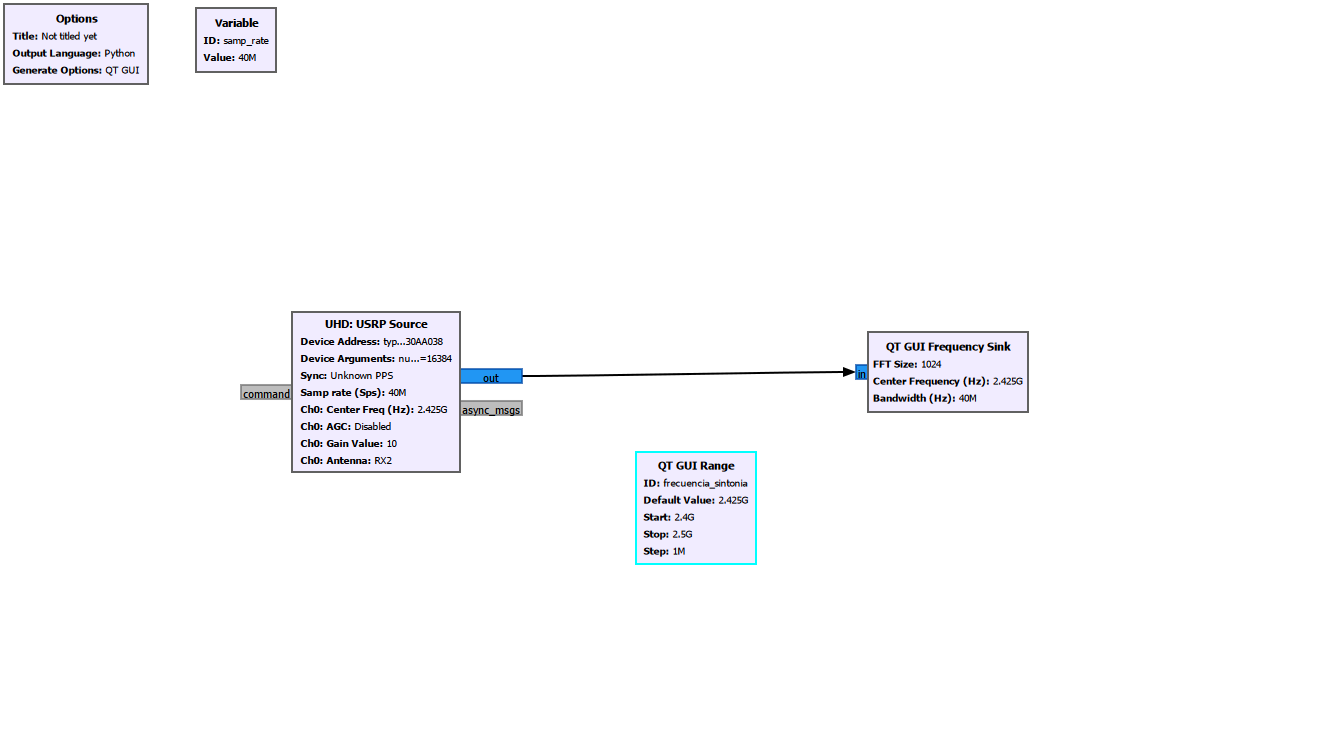
\includegraphics[width=0.95\textwidth]{figuras/implementacion/gnu_osci.png}
    \caption{Flujo de GNU Radio empleado en la fase de búsqueda y sintonía: el receptor USRP alimenta un visor de espectro en tiempo real cuya frecuencia central se controla mediante un deslizador que recorre la banda de \SI{2.4}{\giga\hertz}.}
    \label{fig:gnu_busqueda}
\end{figure}

El flujo de exploración consta de cuatro bloques principales. El bloque \texttt{UHD: USRP Source} configura el receptor: opera sobre el canal~0 con una frecuencia central sintonizable (valor por defecto \SI{2.425}{\giga\hertz}), una tasa de muestreo de \SI{40}{\mega\hertz}, ganancia fija de \num{10}, AGC desactivado y antena RX2. Su salida \texttt{out} se conecta directamente a un bloque \texttt{QT GUI Frequency Sink}, que calcula y muestra el espectro mediante una FFT de \num{1024} puntos sobre un ancho de banda de \SI{40}{\mega\hertz} centrado en la frecuencia sintonizada. Un bloque \texttt{QT GUI Range} (identificador \texttt{frecuencia\_sintonia}) genera un control deslizante que recorre el rango de \SIrange{2.4}{2.5}{\giga\hertz} con paso de \SI{1}{\mega\hertz} y se asocia a la frecuencia central del receptor, de modo que se puede desplazar la sintonía a lo largo de la banda en tiempo real. Finalmente, el bloque \texttt{Variable} fija la tasa de muestreo (\texttt{samp\_rate}~=~\SI{40}{\mega\hertz}) y el bloque \texttt{Options} define la generación del flujo en Python con interfaz QT GUI. A diferencia del flujo de captura, este flujo no almacena datos: su única función es la inspección visual del espectro para localizar la transmisión del dron.

\subsection{Búsqueda del dron en condiciones de alta congestión}

En escenarios de alta congestión RF la localización de la transmisión del dron se complica, ya que numerosos dispositivos WiFi y Bluetooth ocupan simultáneamente la banda. Para reproducir de forma controlada las condiciones más exigentes —las correspondientes al mayor número de dispositivos conectados— se fuerza manualmente al punto de acceso WiFi principal a operar en los canales bajos de la banda (canal~1, centrado en \SI{2412}{\mega\hertz}, o canal~6, en \SI{2437}{\mega\hertz}). Al concentrar la interferencia WiFi en la parte inferior del espectro, el mecanismo de salto de frecuencia adaptativo del enlace OcuSync~O2 tiende a desplazar sus ráfagas hacia la mitad superior de la banda de \SI{2.4}{\giga\hertz}, menos ocupada.

\vspace{1em}
Esta estrategia introduce inicialmente lo que parecía una limitación práctica. Con el ancho de banda instantáneo de \SI{40}{\mega\hertz} del receptor, una única ventana de observación no cubre la totalidad de la banda ISM (\SIrange{2400}{2483.5}{\mega\hertz}), por lo que no es posible centrar de forma perfecta la transmisión del dron: cuando el salto la sitúa cerca de los bordes del rango observado, algunas ráfagas aparecen incompletas o quedan fuera de la ventana. Para maximizar el número de transmisiones del dron efectivamente capturadas bajo interferencia forzada se sintonizaba la frecuencia central del receptor en \SI{2.46}{\giga\hertz}, de modo que la ventana de \SI{40}{\mega\hertz} (\SIrange{2440}{2480}{\mega\hertz}) abarcaba la mitad superior de la banda, donde se concentra la actividad del enlace en estas condiciones.

\vspace{1em}
Sin embargo, a lo largo del trabajo se constató que esa imposibilidad de centrar la señal no es realmente un inconveniente, sino una propiedad deseable para el entrenamiento del detector. En un despliegue real nunca se captura la transmisión del dron perfectamente centrada y aislada: son precisamente las interferencias del entorno las que fuerzan al enlace a aparecer en distintas posiciones y patrones dentro del espectrograma, manteniendo en todo momento sus rasgos morfológicos característicos —las ráfagas FHSS del enlace de mando y las franjas verticales de la transmisión de vídeo OFDM—. Esta variabilidad enriquece el conjunto de datos y permite que la red contraste un mayor número de situaciones. Por ello, en lugar de buscar una única condición ideal, se varió manualmente el canal del WiFi para forzar deliberadamente los saltos del dron y se realizaron medidas a lo largo de toda la banda de \SI{2.4}{\giga\hertz}, incorporando así escenarios marcadamente mixtos en los que las ráfagas del dron y las estructuras WiFi/Bluetooth coexisten en la misma ventana de observación, que son los casos más exigentes para el detector.

\section{Adquisición de señal en GNU Radio}
\label{sec:adquisicion_gnuradio}













\subsection{Estructura del flujo de captura}

El flujo de GNU Radio utilizado para la adquisición tiene una estructura sencilla:

\begin{center}
\texttt{UHD: USRP Source} $\rightarrow$ \texttt{Head} $\rightarrow$ \texttt{SigMF Sink}
\end{center}

El bloque \texttt{UHD: USRP Source} configura el receptor, la frecuencia central, la tasa de muestreo y la ganancia. El bloque \texttt{Head} limita el número de muestras para obtener capturas de duración controlada. Finalmente, el bloque \texttt{SigMF Sink} almacena los datos IQ junto con sus metadatos, permitiendo reproducir posteriormente las condiciones de adquisición.

\subsection{Variables globales}

Las variables principales del flujo son la frecuencia central, la tasa de muestreo, la ganancia y la duración de captura. La campaña utiliza una tasa de muestreo fija $f_s = \SI{40}{\mega\hertz}$ y una ganancia fija de \num{10} con el control automático de ganancia (AGC) desactivado, de modo que el nivel de señal no introduce un sesgo de ganancia entre capturas. Para capturar una duración $T$ con una tasa de muestreo $f_s$, el número de muestras complejas que debe dejar pasar el bloque \texttt{Head} es:

\begin{equation}
N = f_s\, T.
\end{equation}

Por ejemplo, una captura efectiva de \SI{15}{\second} a \SI{40}{\mega\hertz} requiere \num{600e6} muestras complejas, que posteriormente se segmentan en \num{150} espectrogramas de \SI{0.1}{\second}. Fijar $f_s$ y la duración garantiza capturas comparables entre escenarios.

\subsection{Almacenamiento SigMF}

El formato SigMF separa los datos IQ binarios (\texttt{.sigmf-data}) del fichero de metadatos (\texttt{.sigmf-meta}). Esta estructura resulta útil para el TFG porque conserva la información de frecuencia central, tasa de muestreo y formato de muestra. Los scripts de Python leen estos metadatos para reconstruir correctamente el eje de frecuencia absoluta de cada espectrograma, sin asumir valores fijos en el código.




\subsection{Montaje experimental}
\label{sec:montaje_experimental}

El montaje de captura está formado por tres elementos: la antena receptora, el receptor SDR y la fuente de señal. La antena se conecta directamente al USRP B210, conectado por USB 3.0 al equipo de adquisición, que se controla mediante GNU Radio en ejecución. Este receptor permite obtener muestras IQ complejas con un ancho de banda suficiente para observar las estructuras de transmisión de la banda ISM de \SI{2.4}{\giga\hertz}, y almacena las muestras en formato SigMF para su posterior procesado. La configuración de adquisición (antena directional fija, ganancia constante, AGC desactivado y tasa de muestreo de \SI{40}{\mega\hertz}) se mantiene idéntica en los dos tipos de captura, de modo que la única diferencia entre ellos es la fuente de señal presente.

\subsubsection{Captura de dron}

Previamente a capturar los datos IQ recibidos por la antena hay que hacer un trabajo de búsqueda porla banda de 2.4GHz, en la cual nuestro objetivo será encontrar el canal en el que se ha estabilizado la transmisión del dron. Cuando hay pocas interferencias alrededor del dron no es difícil encontrarlo, principalmente por la propia herramienta de visualización de espectro que hemos configurado en GNU radio, en la cual cuando sospechamos que aparecen transmisiones de mucha potencia o burst que nos hagan sospechar que puede haber un dron lo que hacemos es parar la búsqueda y sacamos un archivo de prueba para analizarlo rapidamente. Todo esto es un proceso previo a la captura de datos de manera continua es para encontrar la trasmision




En las capturas de dron, la fuente de señal de interés es el propio dron, que permanece encendido con su enlace de comunicación activo, de modo que sus ráfagas FHSS quedan dentro del lóbulo de la antena directional orientada hacia él. La \cref{fig:setup_antena} ilustra el montaje físico de este tipo de medida. El dron se captura sobre el fondo WiFi del entorno presente durante la campaña, en los niveles de congestión definidos en la \cref{tab:niveles_interferencia}: el objetivo es caracterizar y encontrar la firma del dron como emisor dominante, antes de pasar al escenario mixto con interferencia saturada. 

Una vez confirmamos la presencia del dron gracias a nuestra búsqueda por oscilos

\begin{figure}[H]
    \centering
    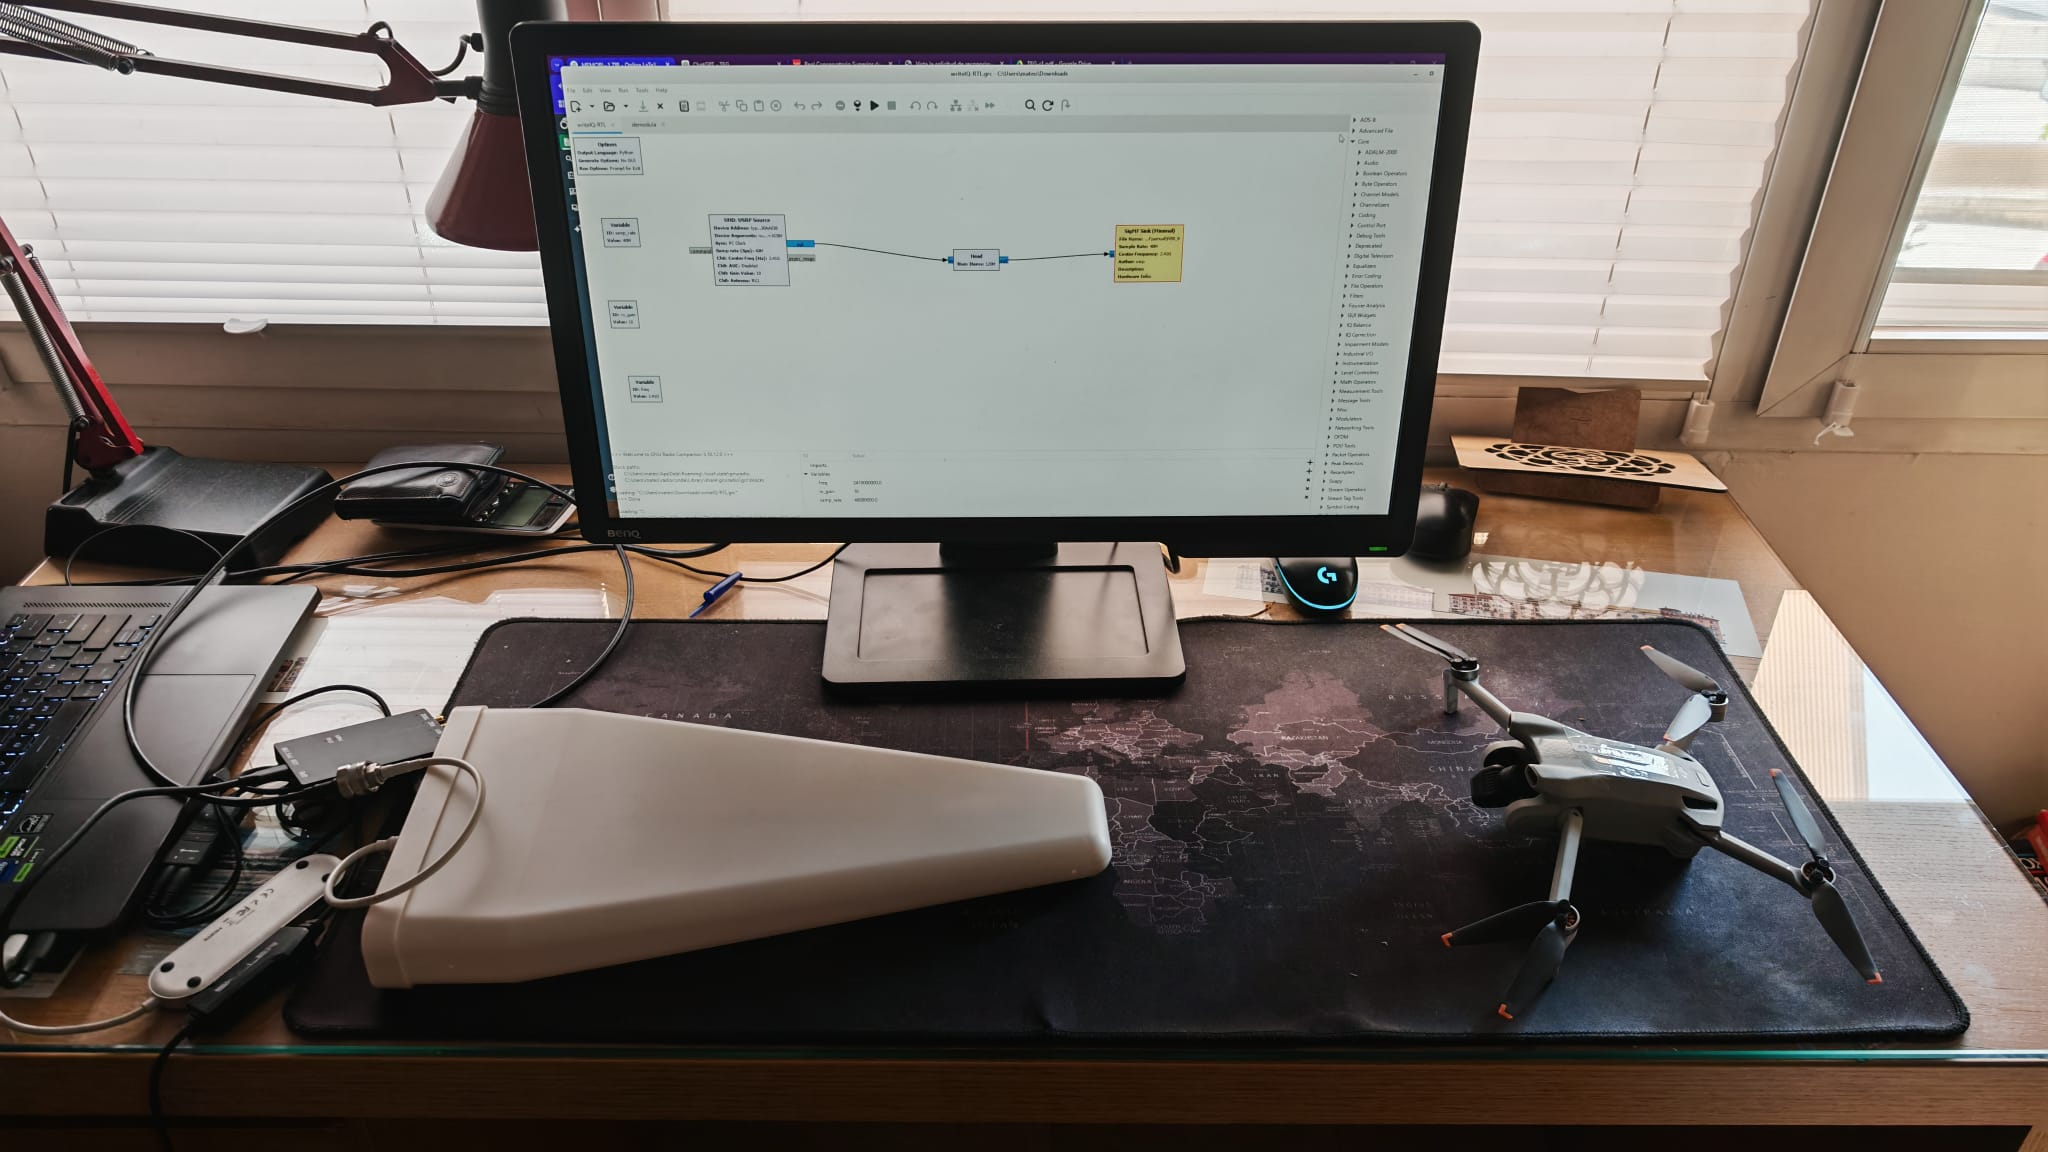
\includegraphics[width=0.85\textwidth]{figuras/implementacion/esquema.jpeg}
    \caption{Montaje experimental para la captura de dron: antena receptora conectada al USRP con GNU Radio en ejecución y el dron como fuente de señal dominante.}
    \label{fig:setup_antena}
\end{figure}

\subsubsection{Captura de interferencia}

En las capturas de interferencia se mantiene exactamente el mismo montaje (antena, posición, ganancia y receptor), pero con el dron apagado. La señal presente procede únicamente de las fuentes de interferencia del entorno, principalmente tráfico WiFi en la banda de \SI{2.4}{\giga\hertz} y, en algunos casos, Bluetooth. Para que la interferencia se reciba con potencia suficiente, los puntos de acceso WiFi se sitúan dentro del lóbulo de la antena directional. Estas capturas se realizan con distintos niveles de congestión para estudiar su efecto, desde tráfico ligero hasta saturación de la banda. Para generar distintos niveles de tráfico WiFi se emplean tanto ordenadores como teléfonos móviles realizando descargas, videollamadas, navegación por internet o vídeo en streaming. Para el Bluetooth se utilizan auriculares, mandos de consola y ratones inalámbricos, que producen ráfagas repartidas en frecuencia con una morfología similar a la del enlace del dron.


Las capturas de interferencia no se realizan en una única condición, sino en tres niveles de congestión creciente de la banda de \SI{2.4}{\giga\hertz}. El objetivo es estudiar cómo afecta la cantidad de tráfico al problema de clasificación, generando la interferencia de forma activa con dispositivos reales para que la ocupación de la banda sea representativa. Los tres niveles se definen aumentando progresivamente el número de fuentes y la intensidad del tráfico:

\begin{itemize}
  \item \textbf{Nivel W1 (bajo):} interferencia ligera. Uno o varios dispositivos reproduciendo vídeo en streaming y un único dispositivo Bluetooth activo o ninguno.
  \item \textbf{Nivel W2 (moderado):} un dispositivo generando tráfico intenso de descarga junto con más de un dispositivo Bluetooth activo.
  \item \textbf{Nivel W3 (alto):} varios dispositivos en descarga y videollamada simultáneas, junto con varios dispositivos Bluetooth activos, saturando la banda.
\end{itemize}

\begin{table}[H]
\centering
\caption{Definición de los tres niveles de interferencia empleados en las capturas.}
\label{tab:niveles_interferencia}
\begin{tabular}{cll}
\toprule
\textbf{Nivel} & \textbf{Tráfico WiFi} & \textbf{Bluetooth} \\
\midrule
W1 & Video streaming & 1 dispositivo \\
W2 & Descarga de alto tráfico & $>$1 dispositivo \\
W3 & Varias descargas + videollamada & Varios dispositivos \\
\bottomrule
\end{tabular}
\end{table}

La inclusión de dispositivos Bluetooth en todos los niveles es deliberada: el Bluetooth también usa saltos de frecuencia (FHSS) con ráfagas de morfología similar a las del dron, por lo que aumenta la dificultad del problema y acerca las capturas al escenario real. El número creciente de fuentes Bluetooth entre W1 y W3 incrementa esa dificultad de forma controlada.

\subsubsection{Captura de entorno mixto}

Las capturas de entorno mixto combinan las dos fuentes anteriores: el dron encendido y, de forma simultánea, las fuentes de interferencia WiFi activas en niveles de congestión altos. Reproducen el escenario realista de despliegue, en el que la señal del dron debe distinguirse en presencia de un fondo RF saturado. El montaje es de nuevo idéntico al de los otros dos casos. 





\begin{figure}[H]
    \centering
    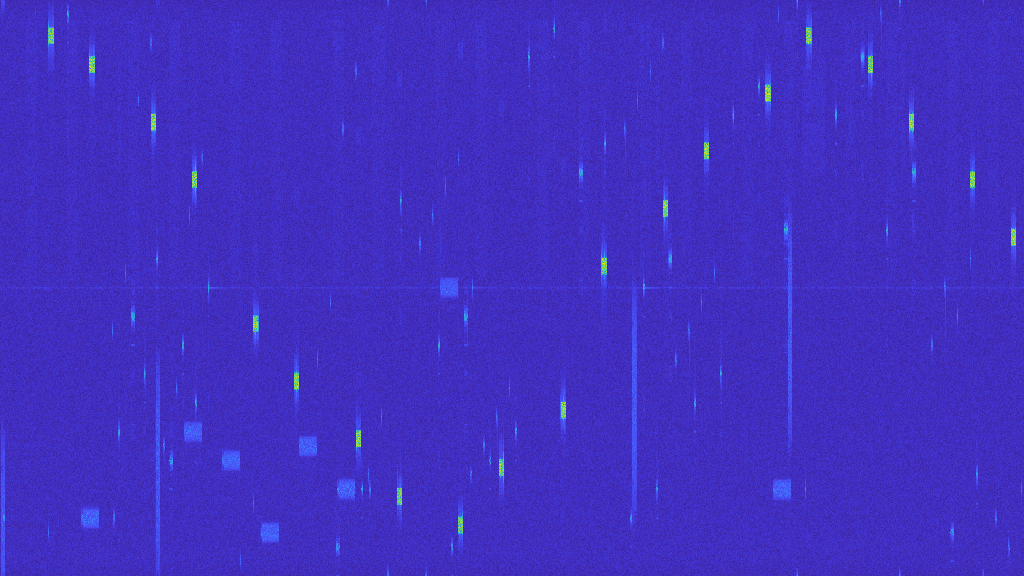
\includegraphics[width=0.85\textwidth]{figuras/implementacion/dronmixto.png}
    \caption{Montaje experimental para la captura en entorno mixto: el dron encendido y las fuentes de interferencia WiFi activas de forma simultánea, reproduciendo el escenario realista de despliegue con fondo RF saturado.}
    \label{fig:setup_mixto}
\end{figure}









\section{Generación de espectrogramas}
\label{sec:generacion_espectrogramas}

La generación de espectrogramas la realiza el script \texttt{make\_spectrogram\_dataset.py}, que convierte cada fichero SigMF en un conjunto de imágenes PNG y registra los metadatos en un CSV maestro.

\subsection{Lectura por segmentos}

Cada fichero SigMF se lee por bloques temporales de \SI{0.1}{\second}. Esta ventana se selecciona porque ofrece un compromiso práctico: es suficientemente corta para generar muchos ejemplos por captura y suficientemente larga para observar patrones de ráfagas y saltos de frecuencia. El número de muestras por segmento es $f_s \cdot \SI{0.1}{\second} = \num{4e6}$ muestras complejas. Cada segmento se lee de forma independiente mediante un acceso por desplazamiento de bytes sobre el fichero binario, sin cargar la captura completa en memoria, y se libera explícitamente la memoria entre segmentos para limitar el consumo de RAM.


\begin{figure}[H]
    \centering
    \begin{subfigure}[b]{0.48\textwidth}
        \centering
        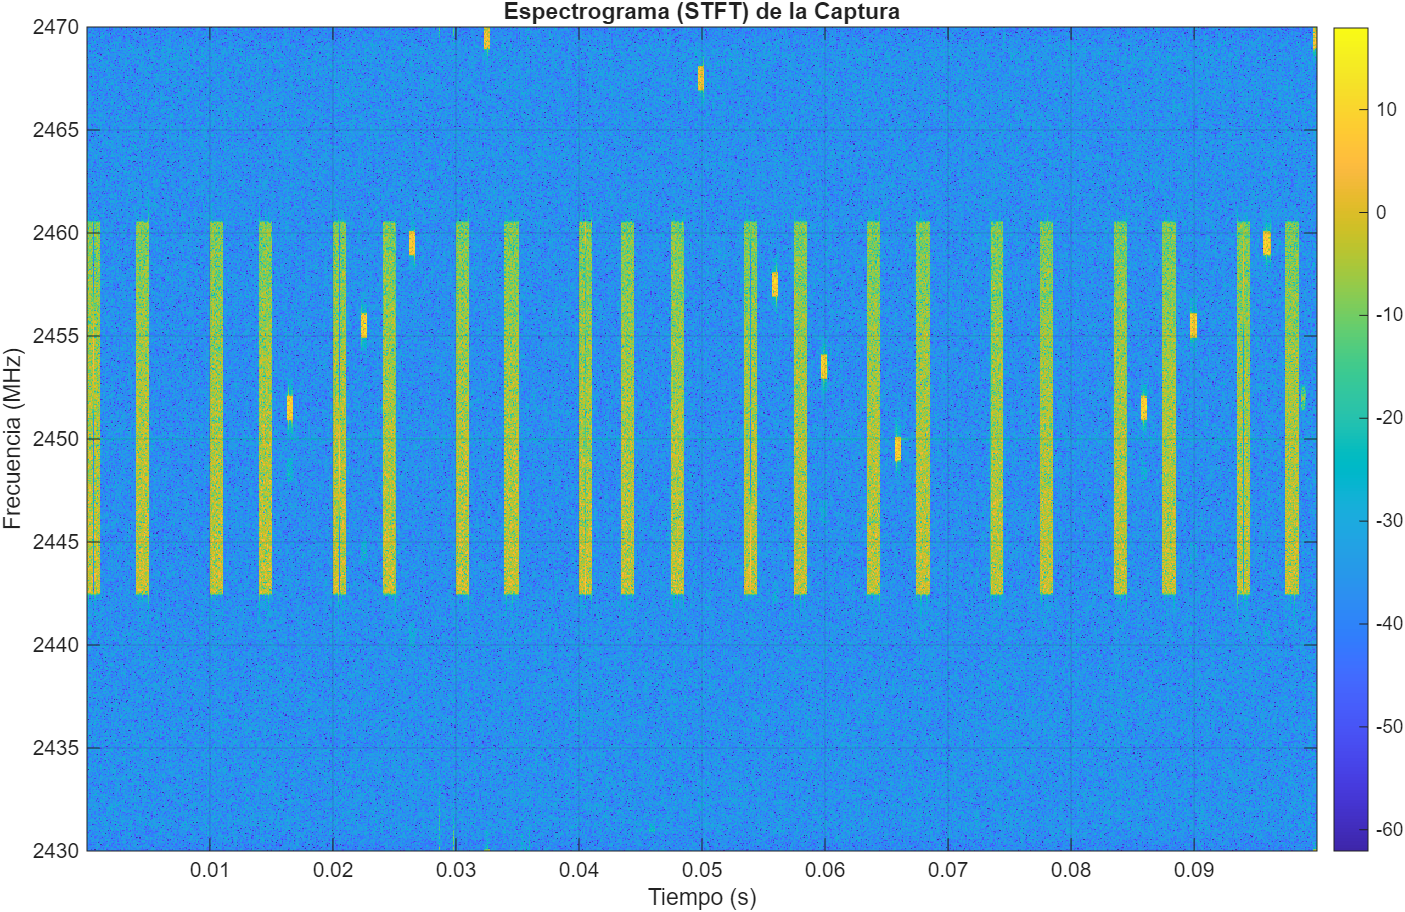
\includegraphics[width=\textwidth]{figuras/requisitos/dron_0_1s.png}
        \caption{Ventana de \SI{0.1}{\second}.}
        \label{fig:espectro_01s}
    \end{subfigure}
    \hfill
    \begin{subfigure}[b]{0.48\textwidth}
        \centering
        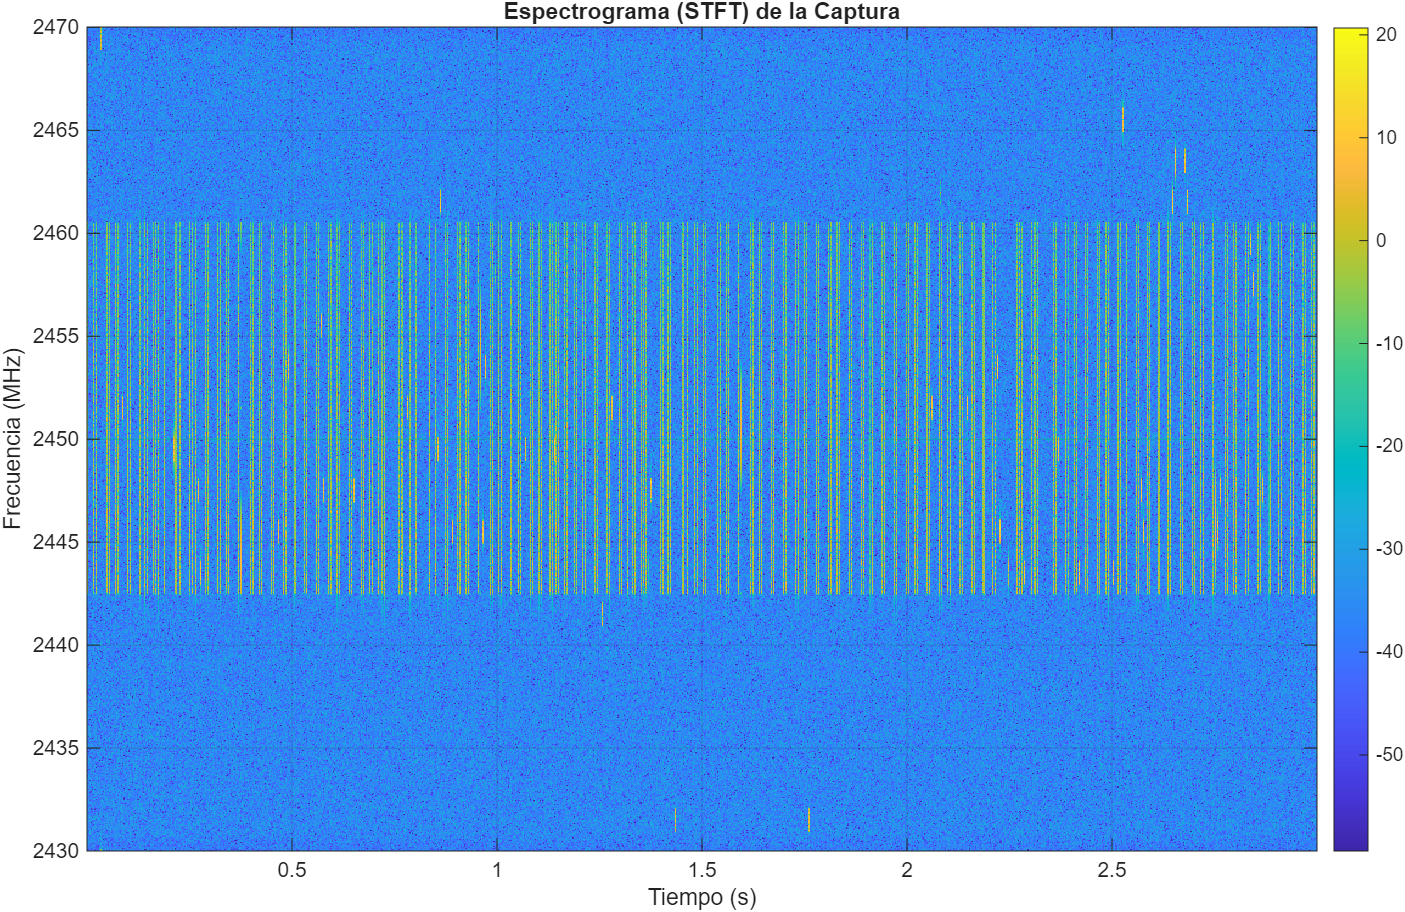
\includegraphics[width=\textwidth]{figuras/requisitos/dron_segundos.png}
        \caption{Ventana de \SI{3}{\second}.}
        \label{fig:espectro_3s}
    \end{subfigure}
    \caption{Comparación de la transmisión del DJI Mini 3 representada con dos ventanas temporales. La ventana corta de \SI{0.1}{\second} (a) resuelve las ráfagas FHSS individuales, mientras que la ventana larga de \SI{3}{\second} (b) las acumula y dificulta distinguir su morfología.}
    \label{fig:comparacion_ventanas}
\end{figure}
\subsection{Cálculo de la STFT}

La representación tiempo-frecuencia se calcula mediante la transformada de Fourier de tiempo corto. Para una señal discreta $x[n]$, la STFT se define como:

\begin{equation}
X(m,k)=\sum_n x[n]\,w[n-mH]\,e^{-j2\pi kn/N},
\end{equation}

donde $w[n]$ es la ventana de análisis, $H$ es el salto entre ventanas, $N$ es el número de puntos de la FFT y $k$ es el índice frecuencial. En la implementación se utiliza una ventana de Hann periódica con $N = \num{1024}$ puntos y un solapamiento del \SI{75}{\percent} ($\num{768}$ muestras). Se calcula el espectro completo de doble banda y se aplica \texttt{fftshift} para centrar la componente de continua, emulando el modo \emph{centered}. Estos parámetros son idénticos en entrenamiento, validación y prueba.

De la STFT se derivan dos resoluciones que determinan el detalle del espectrograma. La \emph{resolución frecuencial} $\Delta f$ es la separación mínima en frecuencia que se puede distinguir, es decir, la anchura de cada bin de la FFT. La \emph{resolución temporal} $\Delta t$ es el intervalo de tiempo más corto que se puede resolver, ligado a la duración de la ventana de análisis. Ambas dependen del número de puntos de la FFT, $N$, y de la tasa de muestreo, $f_s$:

\begin{equation}
\Delta f = \frac{f_s}{N} \approx \SI{39}{\kilo\hertz}, \qquad
\Delta t = \frac{N}{f_s} \approx \SI{25.6}{\micro\second}.
\end{equation}

Existe un compromiso entre ambas: al aumentar $N$ mejora la resolución frecuencial (bins más estrechos) pero empeora la temporal (ventanas más largas), y viceversa. La elección de $N = \num{1024}$ equilibra las dos: ofrece una resolución frecuencial de unos \SI{39}{\kilo\hertz} y una resolución temporal de unos \SI{25.6}{\micro\second}, suficiente para resolver ráfagas FHSS de \SIrange{100}{500}{\micro\second} como las de la señal del dron o del Bluetooth, así como la estructura interna de las tramas WiFi.

La potencia se expresa en decibelios mediante:

\begin{equation}
P_{\mathrm{dB}} = 10\log_{10}\left(|X(m,k)|^2 + \epsilon\right),
\end{equation}

donde $\epsilon$ evita problemas numéricos al tomar el logaritmo de valores cercanos a cero. El eje de frecuencia se expresa en valor absoluto mediante $F_{\mathrm{abs}} = (F + f_c)/10^6$ en MHz, usando la frecuencia central $f_c$ leída de los metadatos SigMF.


El cálculo se implementa con \texttt{scipy.signal.spectrogram}, manteniendo los parámetros descritos:

\begin{lstlisting}[style=python,caption={Cálculo de la STFT de cada segmento.}]
win = windows.hann(NFFT, sym=False)      # Hann periodica, NFFT = 1024
overlap = round(0.75 * NFFT)             # solape del 75%

F, T, S = spectrogram(senal_seg, fs=fs, window=win,
                      nperseg=NFFT, noverlap=overlap, nfft=NFFT,
                      return_onesided=False, mode="complex")

F = np.fft.fftshift(F)                   # centrar la componente de continua
S = np.fft.fftshift(S, axes=0)

Pdb = 10 * np.log10(np.abs(S)**2 + eps)  # potencia en dB
\end{lstlisting}


\subsection{Renderizado y exportación}

Cada espectrograma se exporta como imagen PNG de \num{1024}x\num{576} píxeles a \num{120} ppp usando el mapa de color Parula. La escala de color es automática por imagen, fijada al rango $[\,\text{max}_{\mathrm{dB}} - \SI{80}{\decibel},\ \text{max}_{\mathrm{dB}}\,]$. Mantener el mismo procedimiento de renderizado en todas las particiones asegura que las diferencias aprendidas por el modelo procedan de la señal y no de cambios en la visualización.




\subsection{CSV maestro}

El script genera de forma incremental un CSV maestro con una fila por espectrograma. Las columnas registran el nombre de fichero, la etiqueta, el nivel WiFi, la condición (limpia o mixta), la antena, la distancia, el entorno, la frecuencia central, la tasa de muestreo, la ganancia, el identificador de captura y la plataforma. Estos metadatos permiten construir los splits y analizar resultados por subgrupos.


\subsection{Ejemplo de espectrograma generado}
\label{sec:ejemplo_espectrograma}

La \cref{fig:salto_frecuencia} muestra un espectrograma generado con el procedimiento descrito. En él se aprecia de forma directa el comportamiento de salto de frecuencia de OcuSync: a lo largo de la ventana de \SI{0.1}{\second}, las ráfagas del enlace del dron (regiones brillantes) no se mantienen en una frecuencia fija, sino que se reubican en distintos puntos del espectro, ocupando los huecos libres dentro de la banda de \SI{2.4}{\giga\hertz} y evitando las zonas ocupadas por el WiFi. Las columnas verticales más anchas y tenues corresponden a la ocupación más estable de las señales WiFi, de canal fijo. Cada ráfaga corresponde a una transmisión OFDM del enlace de vídeo, cuya frecuencia central varía de un salto al siguiente. Este patrón es precisamente la firma morfológica que el detector debe aprender a distinguir.

\begin{figure}[H]
    \centering
    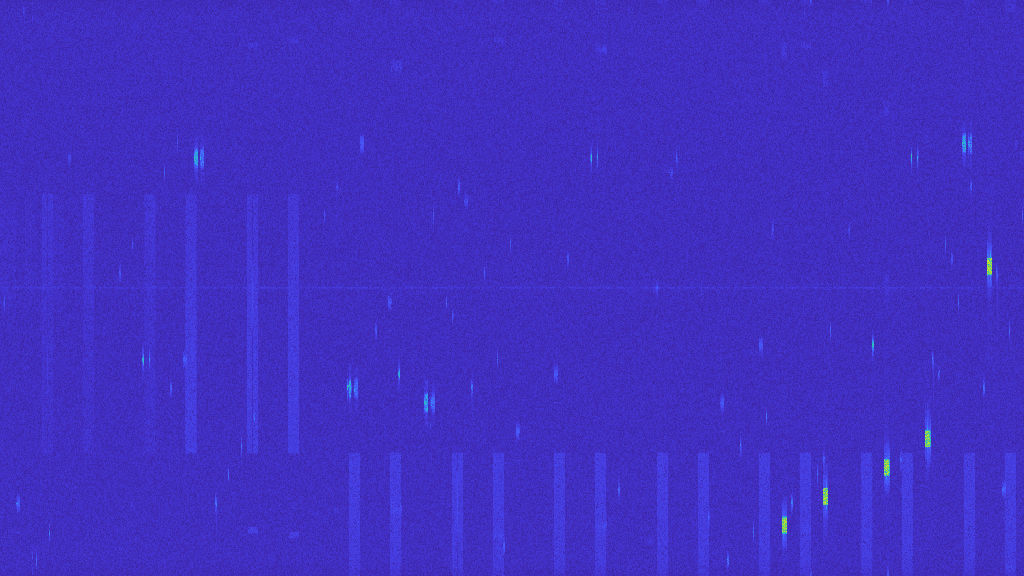
\includegraphics[width=0.9\textwidth]{figuras/implementacion/cambiofrec.png}
    \caption{Espectrograma de \SI{0.1}{\second} generado a partir de una captura del DJI Mini 3. Se observa el salto de frecuencia adaptativo de OcuSync: las ráfagas del enlace del dron aparecen a distintas frecuencias a lo largo de la ventana temporal, mientras que las columnas verticales más anchas y estables corresponden a la actividad WiFi.}
    \label{fig:salto_frecuencia}
\end{figure}





\section{Preparación del dataset YOLO}
\label{sec:preparacion_yolo}

\subsection{Estructura de carpetas}

El dataset para YOLO se organiza en imágenes y etiquetas. Cada imagen PNG tiene asociado un fichero \texttt{.txt} con las cajas delimitadoras en formato YOLO:

\begin{lstlisting}[caption={Formato de una etiqueta YOLO.}]
<class_id> <x_center> <y_center> <width> <height>
\end{lstlisting}

Las coordenadas se normalizan respecto al ancho y alto de la imagen. Las clases utilizadas son \texttt{interference} (clase 0) y \texttt{drone} (clase 1). Además, se genera un fichero \texttt{data.yaml} que define las rutas de entrenamiento, validación y prueba, así como el número y nombre de las clases.




\subsection{Partición por captura}

La partición se realiza con el script \texttt{split\_capture\_level.py} a nivel de captura completa, con proporciones objetivo aproximadas de \num{70}/\num{15}/\num{15} para entrenamiento, validación y prueba, estratificando por etiqueta y con semilla fija \num{42}. Como la partición es por captura entera y no por imagen, el reparto efectivo de espectrogramas no cae exactamente sobre esas proporciones. Este punto es esencial porque los espectrogramas consecutivos de una misma captura comparten condiciones de canal, ganancia, distancia, entorno e interferencias. Si se mezclasen segmentos de una misma captura entre entrenamiento y prueba, la evaluación estaría sesgada por fuga de información. El script incluye una comprobación de no solapamiento que aborta el proceso si algún identificador de captura aparece en más de una partición. No se copian las imágenes entre carpetas: los splits se materializan como listas de rutas relativas.

\section{Auto-etiquetado de ráfagas}
\label{sec:autoetiquetado}

El script \texttt{auto\_label\_bursts.py} genera automáticamente cajas delimitadoras sobre los espectrogramas. El procedimiento se resume en los siguientes pasos:

\begin{enumerate}
  \item leer la imagen del espectrograma;
  \item convertirla a una representación de intensidad y aplicar un suavizado mínimo;
  \item aplicar un umbral en el percentil \num{99.8};
  \item encontrar componentes conectados;
  \item descartar regiones demasiado pequeñas o demasiado grandes;
  \item convertir las cajas al formato YOLO normalizado;
  \item asignar la clase en función de la captura de origen.
\end{enumerate}

La calibración final utiliza un umbral en el percentil \num{99.8}, un área mínima de \num{8} píxeles, un área máxima del \num{0.005} de la imagen, un núcleo morfológico de tamaño \num{1} (sin operación morfológica, para preservar blobs sueltos) y un suavizado gaussiano de $\sigma = \num{0.4}$. Estos valores surgen de un proceso iterativo: las primeras calibraciones (percentil \num{99}, área mínima de \num{200} píxeles, núcleo de tamaño \num{5}) capturaban barras WiFi enteras y las etiquetaban incorrectamente. El filtro final descarta de forma implícita las barras WiFi anchas, que ocupan áreas mucho mayores, y conserva ráfagas FHSS pequeñas compatibles con OcuSync o Bluetooth.

La \cref{fig:yolo_cajas} muestra un ejemplo de espectrograma con sus cajas delimitadoras. Cada caja (en rojo) encierra una ráfaga individual, que es el objeto que el detector debe localizar y clasificar. Obsérvese que las columnas verticales anchas, correspondientes a la actividad WiFi de canal fijo, no quedan enmarcadas: el criterio de área máxima del auto-etiquetado las descarta por su tamaño, de modo que las etiquetas se concentran exclusivamente en las ráfagas estrechas de salto de frecuencia. Esta es precisamente la diferencia frente a un clasificador de imagen completa: al trabajar sobre regiones locales, el modelo atiende a la morfología de cada ráfaga y no al contexto global de la captura.

\begin{figure}[H]
    \centering
    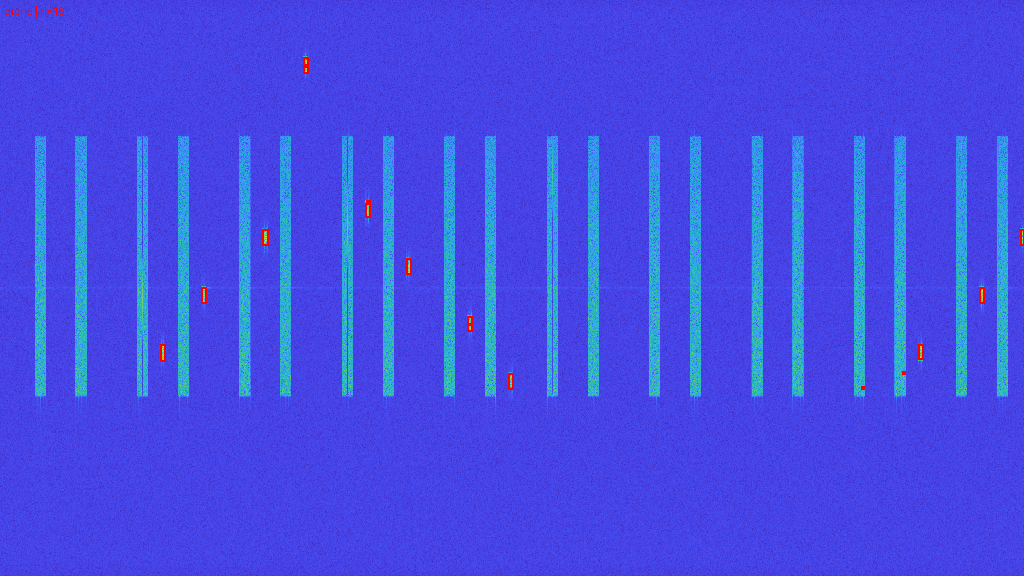
\includegraphics[width=0.9\textwidth]{figuras/implementacion/preview.png}
    \caption{Ejemplo de espectrograma con las cajas delimitadoras en formato YOLO para una captura limpia de dron.}
    \label{fig:yolo_cajas}
\end{figure}


\begin{figure}[H]
    \centering
    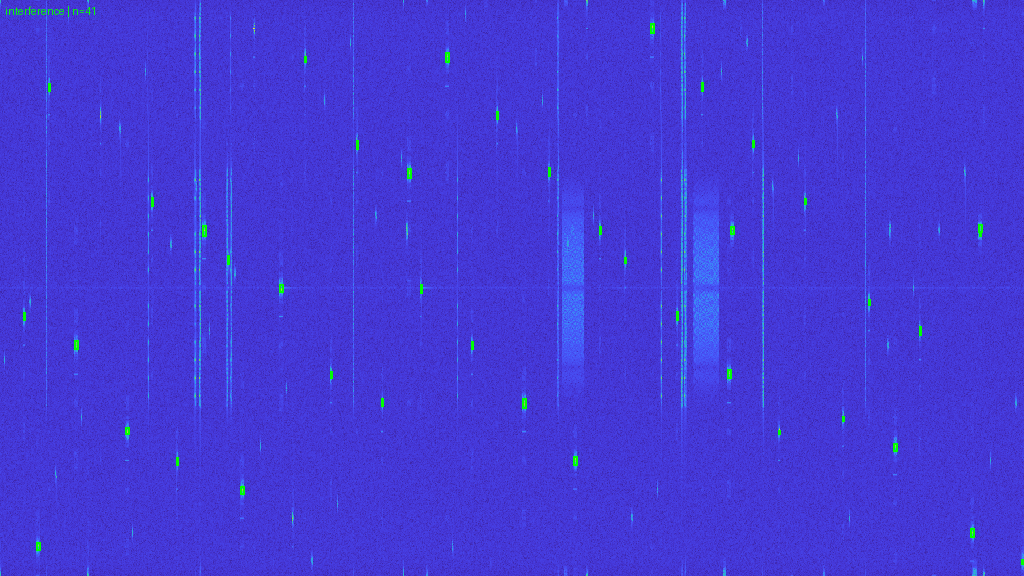
\includegraphics[width=0.9\textwidth]{figuras/implementacion/preview_interference.png}
    \caption{Ejemplo de espectrograma con las cajas delimitadoras en formato YOLO para una captura de interferencia.}
    \label{fig:yolo_cajas_interference}
\end{figure}


La \cref{fig:yolo_cajas_interference} muestra el mismo procedimiento aplicado a una captura sin dron. En este caso, las cajas no se asocian al enlace del dron, sino a las ráfagas dispersas procedentes de Bluetooth y de otras emisiones ISM residuales, que aparecen como pequeños segmentos repartidos por toda la banda y que el auto-etiquetado marca como clase \emph{interference}. Al igual que en la captura de dron, las estructuras verticales más anchas y tenues —atribuibles a la actividad WiFi de canal fijo— quedan descartadas por el criterio de área máxima y no se enmarcan.  La etiqueta \texttt{n=41} indica el número de regiones detectadas en este segmento, evidenciando la densidad de emisores activos en la banda durante la captura.


\subsection{Etiquetado débil y su justificación}

La clase de cada caja se hereda de la captura de origen: las cajas de capturas \texttt{mini3\_drone\_*} se etiquetan como \texttt{drone} y las de capturas \texttt{mini3\_nodrone\_*} como \texttt{interference}. Se trata de un etiquetado débil, pero coherente con el diseño de la campaña: en las capturas de dron no se añaden fuentes Bluetooth dedicadas, por lo que el dron es la fuente FHSS dominante frente al fondo WiFi del entorno, mientras que las capturas sin dron sí incorporan Bluetooth, de modo que las ráfagas detectadas en ellas corresponden a interferencia y no al enlace OcuSync O2. 

\vspace{1em}
Esta coherencia permite entrenar un detector sin anotación manual exhaustiva. No obstante, al asignar la clase por captura completa toda ráfaga de una captura de dron se etiqueta como \texttt{drone} aunque parte de la energía proceda del fondo WiFi, lo que introduce un ruido de etiquetado que se asume como limitación documentada del procedimiento.

\begin{lstlisting}[style=python,caption={Pseudocódigo del auto-etiquetado de ráfagas.}]
img = read_spectrogram(path)
intensity = smooth(to_intensity(img), sigma=0.4)
mask = intensity > percentile(intensity, 99.8)
components = connected_components(mask)

for comp in components:
    box = bounding_box(comp)
    area = box.width * box.height
    if area < min_area_px:            # min_area_px = 8
        continue
    if area > max_area_frac * image_area:   # max_area_frac = 0.005
        continue
    write_yolo_label(box, class_from_capture(path))
\end{lstlisting}





La razón de que el auto-etiquetado conserve únicamente las ráfagas pequeñas, descartando las columnas anchas del WiFi, es metodológica. Distinguir el dron de una señal WiFi es un problema trivial: el WiFi se manifiesta como columnas verticales anchas y fijas, fácilmente separables de cualquier ráfaga de salto de frecuencia mediante descriptores elementales. Un detector que resolviera únicamente esa distinción no demostraría haber aprendido la firma del dron.

El problema científicamente relevante es separar la firma FHSS de OcuSync de otras señales de salto de frecuencia presentes en la banda, en particular del Bluetooth, que comparte con el dron la técnica FHSS y una morfología de ráfagas estrechas y dispersas muy similar. Al filtrar implícitamente las barras WiFi por su tamaño, las ráfagas conservadas en las capturas sin dron corresponden mayoritariamente a Bluetooth. De este modo, la tarea de detección enfrenta dos señales de morfología parecida, y un resultado positivo del modelo evidencia que ha aprendido las diferencias finas entre ambas (ancho de banda por ráfaga, duración y patrón de salto) y no un atajo trivial frente al WiFi. Esto convierte el problema en un banco de pruebas mucho más exigente y representativo del escenario real.

Conviene matizar el papel que desempeña el WiFi en este planteamiento. Aunque sus barras anchas se descartan en el etiquetado y no constituyen la clase que el detector debe separar del dron, la actividad WiFi no es prescindible: su utilidad principal es actuar como agente perturbador del entorno. Por un lado, degrada la calidad de la señal recibida del dron al elevar el nivel de ocupación y de ruido en la banda, reduciendo la relación señal a ruido de sus ráfagas. Por otro, y de forma más determinante, fuerza el mecanismo de salto de frecuencia adaptativo del enlace OcuSync~O2 a reubicar sus transmisiones en los huecos libres del espectro, modificando dinámicamente la posición y el patrón de las ráfagas del dron. De este modo, el WiFi no se trata como una clase a discriminar, sino como el elemento que genera la diversidad de condiciones —distintas posiciones, niveles de potencia y grados de solapamiento— sobre las que el detector debe demostrar que reconoce la firma del dron.


\section{Entrenamiento del detector YOLOv8 (Stage 1)}
\label{sec:entrenamiento_yolo}

El entrenamiento se realiza con YOLOv8n, una variante ligera de aproximadamente tres millones de parámetros. Se parte de pesos preentrenados en COCO y se ajusta el modelo al dataset de espectrogramas mediante \texttt{train\_yolo.py}, un envoltorio sobre Ultralytics. La configuración principal es:

\begin{table}[htbp]
\centering
\caption{Configuración principal del entrenamiento YOLOv8n.}
\label{tab:config_yolo}
\begin{tabular}{ll}
\toprule
\textbf{Parámetro} & \textbf{Valor} \\
\midrule
Modelo base & \texttt{yolov8n.pt} \\
Tamaño de entrada & \num{640}x\num{640} \\
Batch size & 16 \\
Épocas finales & 60 \\
Semilla & 42 \\
Optimizador & Automático de Ultralytics \\
Clases & \texttt{interference}, \texttt{drone} \\
\bottomrule
\end{tabular}
\end{table}

Las aumentaciones geométricas se limitan para respetar la física del espectrograma. No se aplican inversiones, rotaciones, \emph{shear} ni perspectiva, ya que los ejes de tiempo y frecuencia tienen significado físico y no pueden invertirse. Se permiten únicamente pequeñas traslaciones o escalados que no destruyen la relación temporal y frecuencial de la señal.

\section{Clasificación de presencia a nivel de imagen}
\label{sec:implementacion_presencia}

Las métricas estándar de YOLO (mAP, recall a nivel de caja) evalúan la calidad geométrica de la detección, pero no responden directamente a la pregunta operativa del trabajo: dada una ventana de \SI{0.1}{\second}, ¿hay dron o no? El script \texttt{presence\_analysis.py} implementa un clasificador de presencia a nivel de imagen sobre las predicciones del detector.

Para una imagen $I$, sea $B_d(I)$ el conjunto de cajas predichas con clase \texttt{drone} y confianza mayor o igual que un umbral $\mathit{thr}$. Se define la verdad de campo $\mathrm{GT}(I) = 1$ si la imagen procede de una captura de dron, y la predicción de presencia:

\begin{equation}
\mathrm{Pred}(I) = 1 \iff |B_d(I)| \ge K,
\end{equation}

donde $K$ es el número mínimo de cajas \texttt{drone} que deben superar el umbral. Los dos hiperparámetros operativos son el umbral de confianza $\mathit{thr}$ y el mínimo de ráfagas $K$. Con la pareja $(\mathrm{GT}, \mathrm{Pred})$ por imagen se construye una matriz de confusión binaria de la que se derivan exactitud, precisión, recall, especificidad y F1. El script realiza un barrido bidimensional sobre $\mathit{thr}$ y $K$; los resultados numéricos se presentan en el \cref{cap:pruebas_resultados}.

\section{Segunda etapa de clasificación (Stage 2)}
\label{sec:implementacion_stage2}

La segunda etapa clasifica el modelo de dron mediante una red convolucional ResNet18 con aprendizaje por transferencia. A diferencia del enfoque inicial, esta clasificación no sustituye a la detección, sino que es una etapa posterior condicionada a la presencia de señal de dron. El clasificador implementado distingue seis clases: \texttt{f450}, \texttt{hunter}, \texttt{mavic\_video}, \texttt{mavic\_novideo}, \texttt{mini3} e \texttt{interference}.

La red parte de pesos preentrenados en ImageNet y sustituye la capa final por una cabeza lineal de seis salidas. Las transformaciones de entrada son las mismas que en el resto del sistema: \texttt{FrequencyNormalize} (recorte centrado en el pico de energía, \texttt{window\_frac}=\num{0.5}), redimensionado a \num{224}x\num{224} y normalización con las estadísticas de ImageNet. El mejor modelo se guarda como \texttt{best\_model.pth} y se reutiliza tanto para la evaluación como para el barrido de robustez. En el pipeline completo, el flujo es:

\begin{enumerate}
  \item YOLO detecta regiones \texttt{drone} en el espectrograma;
  \item se selecciona el espectrograma asociado a la detección;
  \item el clasificador ResNet18 predice el modelo de dron.
\end{enumerate}

Esta separación permite que cada red resuelva un problema distinto: YOLO responde a la pregunta de presencia y localización, mientras que ResNet18 responde a la identificación del modelo.

\section{Barrido de robustez frente a ruido (SNR)}
\label{sec:implementacion_snr}

Para cuantificar la degradación del clasificador Stage 2 ante contaminación RF sin necesidad de capturar más datos, se inyecta ruido sintético en el dominio IQ con potencia calibrada a un SNR objetivo y se regenera el espectrograma con el mismo pipeline de entrenamiento. Se implementan dos modelos de ruido en \texttt{snr\_noise.py}.

\subsection{Ruido AWGN}

Ruido blanco gaussiano complejo $n[k] \sim \mathcal{CN}(0, \sigma^2)$, con la varianza calibrada al SNR objetivo a partir de la potencia media de la señal:

\begin{equation}
P_{\mathrm{signal}} = \frac{1}{L}\sum_k |x[k]|^2, \qquad
P_{\mathrm{noise}} = \frac{P_{\mathrm{signal}}}{10^{\,\mathrm{SNR}/10}}, \qquad
\sigma = \sqrt{\frac{P_{\mathrm{noise}}}{2}}.
\end{equation}

Es el modelo canónico de ruido térmico de receptor y reparte su energía uniformemente por todo el plano tiempo-frecuencia.

\subsection{Interferencia FHSS sintética}

Modela una interferencia tipo Bluetooth Classic. Por cada segmento de \SI{0.1}{\second} se generan unos \num{160} bursts ($\num{1600}$ hops/s $\times$ \SI{0.1}{\second}), cada uno de \SI{366}{\micro\second} de duración y \SI{1}{\mega\hertz} de ancho, situados en frecuencias aleatorias dentro del \SI{90}{\percent} del ancho de banda capturado. Cada burst usa una modulación GFSK simplificada (chirp lineal de $\pm\SI{250}{\kilo\hertz}$ con sentido aleatorio) y una ventana de Hann en amplitud. La energía total se escala para cumplir el mismo SNR objetivo que el AWGN, de modo que la \emph{única} diferencia entre ambos ruidos es la distribución espacial de la energía en el plano tiempo-frecuencia. Esta condición es la más exigente porque comparte morfología FHSS con la señal del dron.

\subsection{Renderizado y barrido}

El script \texttt{spectrogram\_render.py} regenera espectrogramas en memoria replicando uno a uno los parámetros de \texttt{make\_spectrogram\_dataset.py}, mediante una tabla de color Parula precalculada para evitar el coste de \texttt{matplotlib}. El script \texttt{snr\_sweep\_stage2.py} recorre, para cada imagen del conjunto de test, cada tipo de ruido y cada SNR del rango $\{+\infty, +20, +15, +10, +5, 0, -5, -10, -15, -20\}$ dB: localiza el fichero SigMF, lee el segmento IQ, inyecta el ruido calibrado, renderiza el espectrograma, aplica las transformaciones del modelo y obtiene la predicción. El SNR de $+\infty$ actúa como control sin ruido y debe reproducir las métricas del test original. Finalmente, \texttt{plot\_snr\_sweep.py} genera las curvas y matrices de confusión. Los resultados se presentan en el \cref{cap:pruebas_resultados}.
% =============================================================================
% Capitulo 5 - Pruebas y resultados
% =============================================================================
\chapter{Pruebas y resultados}
\label{cap:pruebas_resultados}

% =============================================================================
\section{Preguntas de investigación}
\label{sec:preguntas_investigacion}

El sistema desarrollado en este trabajo comprende dos etapas encadenadas: una primera etapa de detección de ráfagas FHSS mediante YOLOv8, y una segunda etapa de clasificación de modelos de dron mediante ResNet18. Este capítulo valida ambas etapas respondiendo a cuatro preguntas de investigación, presentadas en el orden en que surgieron a lo largo del trabajo:

\begin{enumerate}
  \item \textbf{P1 ---} ¿Puede un clasificador global distinguir espectrogramas con señal de dron de los que contienen únicamente interferencia?
  \item \textbf{P2 ---} ¿Puede un detector de objetos localizar y separar morfológicamente las ráfagas FHSS de OcuSync de las interferencias presentes en la banda de \SI{2.4}{\giga\hertz}?
  \item \textbf{P3 ---} ¿Permiten las detecciones anteriores confirmar operativamente la presencia de un dron en una ventana temporal de \SI{0.1}{\second}?
  \item \textbf{P4 ---} ¿Puede el sistema identificar el modelo concreto de dron y discrimina su decisión por la morfología espectro-temporal de las ráfagas o por el nivel medio de potencia?
\end{enumerate}

Las dos primeras articulan la evolución metodológica del trabajo: la primera establece que la firma OcuSync es aprendible pero motiva el paso a un detector de objetos, y la segunda evalúa ese detector. Las dos últimas cuantifican el rendimiento operativo y la solidez del sistema definitivo.

Para cada pregunta se expone la descripción del experimento, los resultados obtenidos y una discusión de los mismos. Las métricas específicas de cada bloque se definen en el apartado correspondiente, junto con el experimento que las emplea.

% =============================================================================
\section{Conjunto de datos de evaluación}
\label{sec:dataset_evaluacion}

Las preguntas P1, P2 y P3 se responden sobre el dataset~v3 cuya captura, composición y generación de espectrogramas se describen en el \cref{cap:implementacion}. El conjunto consta de \num{3150}~espectrogramas de \num{1024}×\num{576}~píxeles, particionados por captura completa para evitar fuga de información entre particiones (véase \cref{subsec:diseno_dataset}). El conjunto de prueba comprende \num{600}~imágenes con balance exacto de \num{300}~\emph{drone} y \num{300}~\emph{interference}, y es el que se emplea para reportar todos los resultados de test de este capítulo. La pregunta~P4 emplea adicionalmente un conjunto de capturas de campo abierto con drones reales, descrito al inicio de la \cref{sec:bloque_clasificacion}.

% =============================================================================

% =============================================================================
% P1 --- version revisada: GradCAM como evidencia de que la clasificacion
% global NO se apoya en la morfologia de las rafagas.
% Sustituye integramente la seccion P1 del capitulo 5.
% Figuras nuevas: resnet18_gradcam_drone.png y resnet18_gradcam_interference.png
% (versiones de dos columnas: Entrada | GradCAM de la clase verdadera).
% =============================================================================

\section{P1 --- ¿Es reconocible la firma OcuSync mediante clasificación global?}
\label{sec:bloque_resnet_detector}

\subsection{Planteamiento del experimento}
\label{sec:p1_planteamiento}

La primera aproximación al problema consiste en entrenar un clasificador binario ResNet18 sobre el espectrograma completo para asignar la etiqueta \emph{drone} o \emph{interference} a cada imagen. Esta formulación evita la complejidad del etiquetado regional: basta con la etiqueta de la captura de la que procede cada espectrograma.

Se parte de una ResNet18 preentrenada en ImageNet, congelando las primeras tres capas y sustituyendo la cabeza de clasificación original por una capa \texttt{Linear(512,~2)}. El modelo se entrena durante \num{20}~épocas con el optimizador AdamW (tasa de aprendizaje \num{1e-4}, \emph{weight decay} \num{1e-4}), planificador \texttt{CosineAnnealingLR} y tamaño de lote \num{32}. Se aplica la normalización frecuencial \texttt{FrequencyNormalize} y la semilla se fija en 42.

\subsection{Resultados}
\label{sec:p1_resultados}

La \cref{fig:resnet18_binary_curvas} muestra la evolución de la pérdida y el F1~macro en entrenamiento y validación a lo largo de las veinte épocas.

\begin{figure}[htbp]
    \centering
    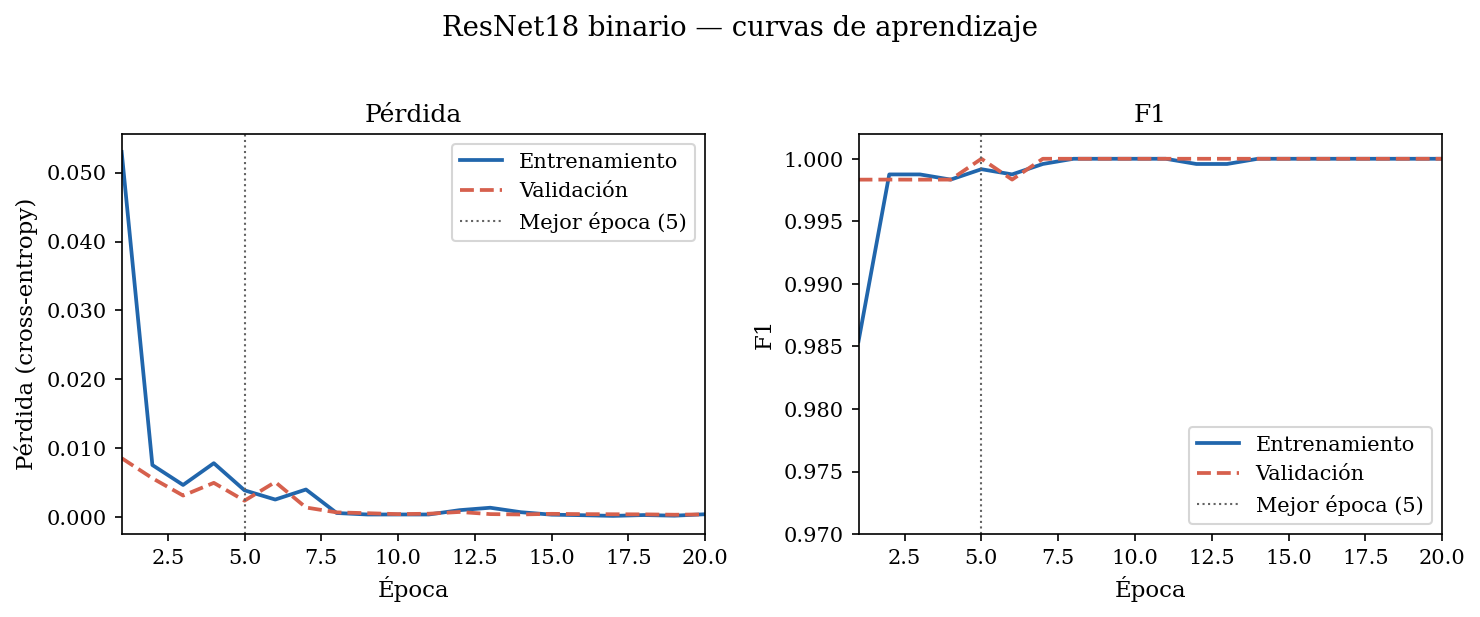
\includegraphics[width=0.85\textwidth]{figuras/resultados/resnet18_binary_curvas.png}
    \caption{Evolución de la pérdida y el F1~macro en entrenamiento y validación del clasificador ResNet18 binario a lo largo de las veinte épocas. La convergencia es extremadamente rápida: en menos de cinco épocas el F1 de validación alcanza \num{1,000}. La pérdida de validación se sitúa consistentemente por debajo de la de entrenamiento, lo que es habitual cuando el \emph{dropout} penaliza la pasada de entrenamiento pero no la de validación. No se observa sobreajuste en las curvas.}
    \label{fig:resnet18_binary_curvas}
\end{figure}

El modelo converge en menos de cinco épocas. La \cref{tab:p1_curva} detalla los valores de las primeras ocho épocas. En las épocas~1 a~4 el clasificador comete exactamente un error sobre las \num{450}~muestras de validación (F1~val = 0,998), que corresponde a una única muestra de interferencia con ráfagas Bluetooth morfológicamente próximas a OcuSync. Este error desaparece en la época~5, a partir de la cual el F1~de validación alcanza \num{1,000} con oscilaciones mínimas (una vuelta a \num{0,998} en la época~6, seguida de estabilización en \num{1,000} a partir de la época~7).

\begin{table}[htbp]
\centering
\caption{Pérdida y F1~macro durante las primeras ocho épocas del clasificador ResNet18 binario.}
\label{tab:p1_curva}
\begin{tabular}{ccccc}
\toprule
\textbf{Época} & \textbf{Loss train} & \textbf{F1 train} & \textbf{Loss val} & \textbf{F1 val} \\
\midrule
1 & 0,0530 & 0,985 & 0,0085 & 0,998 \\
2 & 0,0075 & 0,999 & 0,0056 & 0,998 \\
3 & 0,0046 & 0,999 & 0,0031 & 0,998 \\
4 & 0,0078 & 0,998 & 0,0050 & 0,998 \\
5 & 0,0039 & 0,999 & 0,0024 & 1,000 \\
6 & 0,0025 & 0,999 & 0,0051 & 0,998 \\
7 & 0,0040 & 1,000 & 0,0014 & 1,000 \\
8 & 0,0006 & 1,000 & 0,0007 & 1,000 \\
\bottomrule
\end{tabular}
\end{table}

El \emph{checkpoint} de la época~5 se evalúa sobre el conjunto de prueba con los resultados de la \cref{tab:p1_test}. La clasificación es perfecta en todas las métricas: las \num{300}~muestras de la clase \emph{drone} y las \num{300}~de \emph{interference} se asignan correctamente, sin errores en ninguna dirección.

\begin{table}[htbp]
\centering
\caption{Resultados del clasificador ResNet18 binario sobre el conjunto de prueba (\num{600}~espectrogramas, \emph{checkpoint} época~5).}
\label{tab:p1_test}
\begin{tabular}{lc}
\toprule
\textbf{Métrica} & \textbf{Valor} \\
\midrule
Exactitud         & 1,000 \\
F1~macro          & 1,000 \\
Precisión macro   & 1,000 \\
Recall macro      & 1,000 \\
\bottomrule
\end{tabular}
\end{table}

\subsubsection{¿Dónde mira la red? Análisis GradCAM}
\label{sec:p1_gradcam}

La clasificación perfecta de la \cref{tab:p1_test} no informa de \emph{por qué} la red decide como decide. Una exactitud del \SI{100}{\percent} es compatible tanto con un modelo que aprende la morfología de las ráfagas FHSS como con un modelo que explota cualquier diferencia sistemática entre las dos clases ajena a la señal. Para discriminar entre ambas hipótesis se aplica GradCAM sobre muestras del conjunto de prueba.

GradCAM calcula el gradiente de la puntuación de la clase respecto a los mapas de activación de la última capa convolucional (\texttt{layer4} de la ResNet18) y los combina ponderadamente para producir un mapa de calor sobre la imagen de entrada. Las regiones con mayor activación son las que más contribuyen a la predicción: si el clasificador resolviera la decisión a partir de la firma OcuSync, el mapa de calor debería concentrarse sobre las ráfagas FHSS verticales y diferir claramente entre una captura de dron y una de interferencia.

La \cref{fig:resnet18_gradcam_drone} muestra el resultado para cuatro espectrogramas de la clase \emph{drone}, y la \cref{fig:resnet18_gradcam_interference} para cuatro de la clase \emph{interference}. En ambas figuras la columna izquierda es la entrada tras la normalización frecuencial y la derecha el mapa GradCAM de la clase verdadera de cada fila superpuesto sobre esa misma entrada.

\begin{figure}[htbp]
    \centering
    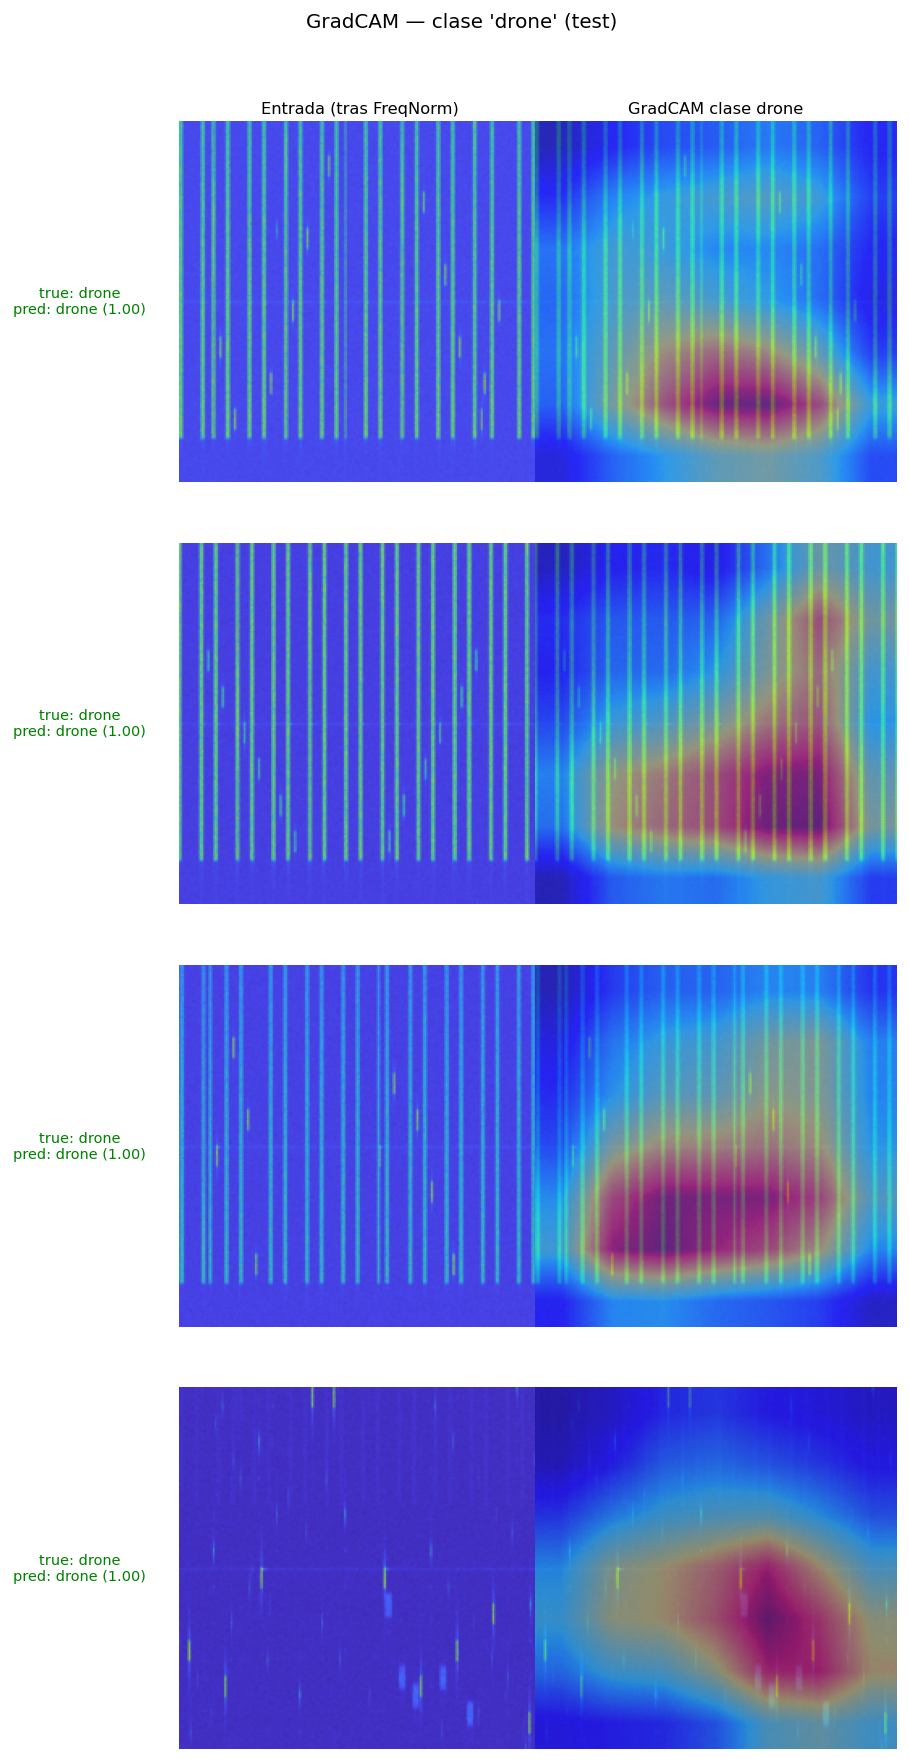
\includegraphics[width=0.80\textwidth]{figuras/resultados/gradcam_drone.png}
    \caption{GradCAM del clasificador ResNet18 binario sobre cuatro espectrogramas de la clase \emph{drone}. Izquierda: Ráfagas FHSS verticales de OcuSync claramente visibles. Derecha: mapa de calor de la clase \emph{drone}. }
    \label{fig:resnet18_gradcam_drone}
\end{figure}

\begin{figure}[htbp]
    \centering
    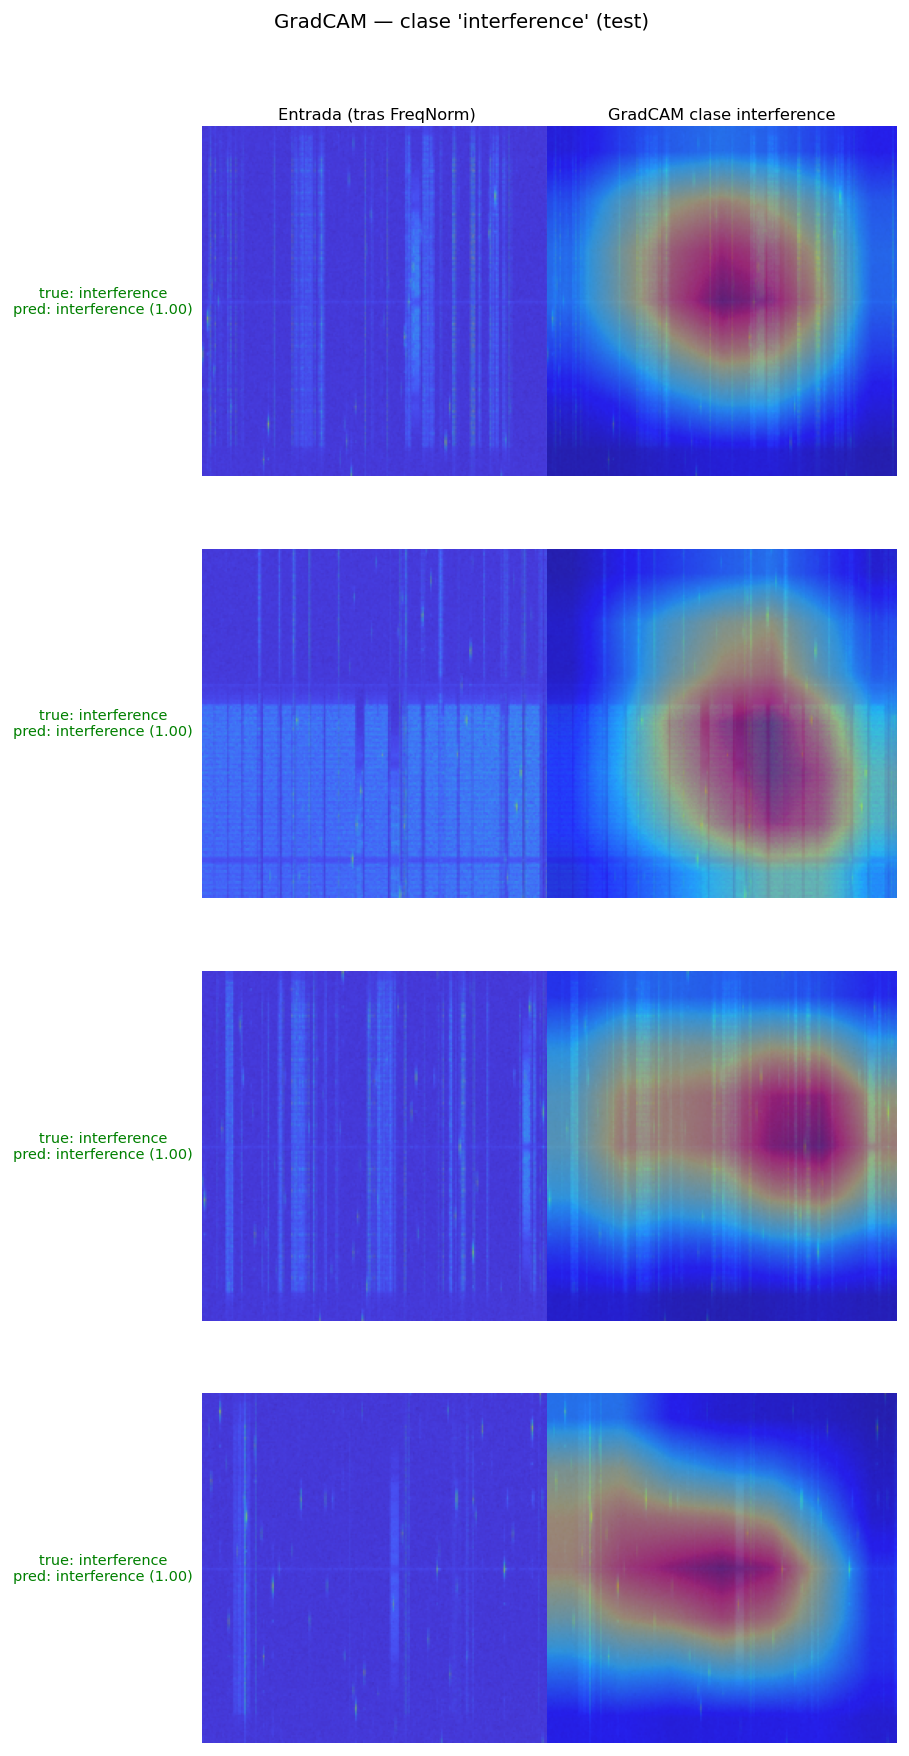
\includegraphics[width=0.80\textwidth]{figuras/resultados/gradcam_interference.png}
    \caption{GradCAM del clasificador ResNet18 binario sobre cuatro espectrogramas de la clase \emph{interference}. Izquierda: entrada tras \texttt{FrequencyNormalize}, con señales WiFi y Bluetooth dispersas y de menor energía. Derecha: mapa de calor de la clase \emph{interference}.}
    \label{fig:resnet18_gradcam_interference}
\end{figure}

El resultado es revelador y contrario a lo que cabría esperar de un modelo que hubiese aprendido la firma RF. En las capturas de dron (\cref{fig:resnet18_gradcam_drone}) la activación no recae sobre las ráfagas FHSS: forma una mancha difusa y suave en la región central-inferior que ignora la estructura vertical periódica de OcuSync y deja fuera las ráfagas de los bordes. En las capturas de interferencia (\cref{fig:resnet18_gradcam_interference}) el mapa de calor es esencialmente el mismo --- una mancha central de forma y posición casi indistinguibles --- a pesar de que el contenido de las dos imágenes no tiene nada en común.

La conclusión es directa: \textbf{los dos mapas de calor son prácticamente iguales entre clases}. Si la red estuviera discriminando por la morfología de la señal, el GradCAM de cada clase debería localizarse sobre estructuras distintas; en cambio, ambas predicciones se sustentan sobre la misma región central genérica de la imagen. GradCAM no consigue señalar ninguna evidencia local, específica de clase, que justifique la decisión. El clasificador alcanza F1\,=\,\num{1,000}, pero su atención no está anclada a la firma OcuSync, sino a un atributo difuso y global del espectrograma.

\subsection{Discusión}
\label{sec:p1_discusion}

El experimento P1 deja dos conclusiones. Por un lado, confirma que las dos clases son perfectamente separables con la información del espectrograma completo: la exactitud del \SI{100}{\percent} demuestra que existe alguna característica que distingue sin error una captura con dron de una de interferencia. Por otro lado, el análisis GradCAM demuestra que \textbf{esa característica no es la morfología de las ráfagas FHSS}. Una exactitud perfecta acompañada de mapas de saliencia difusos e idénticos entre clases es la huella típica de un clasificador que ha aprendido un atributo global de la captura --- nivel medio de potencia, brillo de fondo, condiciones del entorno de grabación --- correlacionado con la etiqueta pero ajeno a la señal del dron.


Este hallazgo es precisamente lo que invalida la clasificación global como criterio de detección, por tres motivos que se refuerzan entre sí.

El primero es la falta de auditabilidad. Un sistema de vigilancia debe poder justificar cada alarma señalando la evidencia concreta que la motiva. Un clasificador cuyo GradCAM apunta a una mancha central inespecífica no ofrece ninguna justificación verificable: no se puede saber qué parte de la señal ha disparado la decisión, ni distinguir una detección legítima de una casualidad estadística del conjunto de datos.


El segundo es la fragilidad ante el cambio de dominio. Si la decisión se apoya en un atributo global del entorno de captura y no en la firma RF, basta con que cambien las condiciones de grabación --- otra ganancia, otro recinto, exterior en lugar de interior --- para que la correlación aprendida se rompa y el rendimiento se desplome, aun cuando la señal del dron sea idéntica. La poca variabilidad intraclase del dataset~v3 (un único modelo de dron, un único entorno interior) hace que el atajo sea especialmente fácil de aprender y, por tanto, especialmente engañoso: el F1\,=\,\num{1,000} mide la capacidad de separar \emph{estas} capturas, no la de reconocer la firma de un dron en general.


El tercero es la ausencia de localización y de aprendizaje multietiqueta. El clasificador emite una única etiqueta para toda la imagen, de modo que no puede indicar en qué región del espectrograma está la señal ni representar la coexistencia de dron e interferencia en la misma ventana temporal, una situación habitual en un escenario real.


En conjunto, P1 demuestra que la pregunta «¿es la firma OcuSync separable?» tiene respuesta afirmativa, pero que un clasificador global no es la herramienta adecuada para responderla de forma fiable: acierta por las razones equivocadas. Estas limitaciones motivan directamente el experimento P2 --- reformular la tarea como detección de objetos ---, que obliga al modelo a justificar cada predicción con la región concreta del espectrograma que la soporta y, con ello, a aprender la morfología local de las ráfagas en lugar de un atajo contextual.








%=========================================================
\section{P2 --- ¿Puede YOLOv8 localizar y separar morfológicamente las ráfagas FHSS?}
\label{sec:bloque_yolo}

\subsection{Planteamiento del experimento}
\label{sec:p2_planteamiento}

El segundo experimento reformula el reconocimiento de señales como un problema de detección de objetos. En lugar de asignar una etiqueta global a cada espectrograma, el modelo debe generar cajas delimitadoras sobre las ráfagas individuales del plano tiempo-frecuencia y clasificar cada una como \emph{drone} (ráfaga OcuSync) o \emph{interference} (ráfaga WiFi/Bluetooth). Las etiquetas se generan con el auto-etiquetado descrito en la \cref{sec:autoetiquetado} (umbral percentil 99,8, etiquetado débil por captura), y el detector se configura según la \cref{sec:entrenamiento_yolo} (YOLOv8n, entrada 640×640, lote~16, sin aumentaciones geométricas).

Se realizan dos entrenamientos sobre el mismo dataset: una primera tanda de \num{15}~épocas como referencia inicial, y una segunda tanda de \num{60}~épocas como modelo final.

Las métricas de precisión, recall y mAP se definen en la \cref{subsec:diseno_evaluacion}. Conviene precisar aquí la distinción entre métricas globales y por clase: el \textbf{mAP@50 global} promedia la precisión media de cada clase activa sobre el conjunto de prueba; el \textbf{mAP@50 por clase} permite comparar directamente el rendimiento del detector sobre \emph{drone} frente a \emph{interference}. La \textbf{puntuación de confianza} (\emph{confidence score}) es el valor entre 0 y 1 que el modelo asigna a cada detección; se emplea como umbral de filtrado para controlar el equilibrio entre precisión y recall, y su elección óptima se determina a partir de la curva F1-confianza mostrada en los resultados.

\subsection{Resultados}
\label{sec:p2_resultados}

\paragraph{Evolución del entrenamiento.}

La \cref{fig:yolo_run02_results} muestra las curvas de pérdida y métricas de validación a lo largo de las \num{60}~épocas del modelo final.

\begin{figure}[htbp]
    \centering
    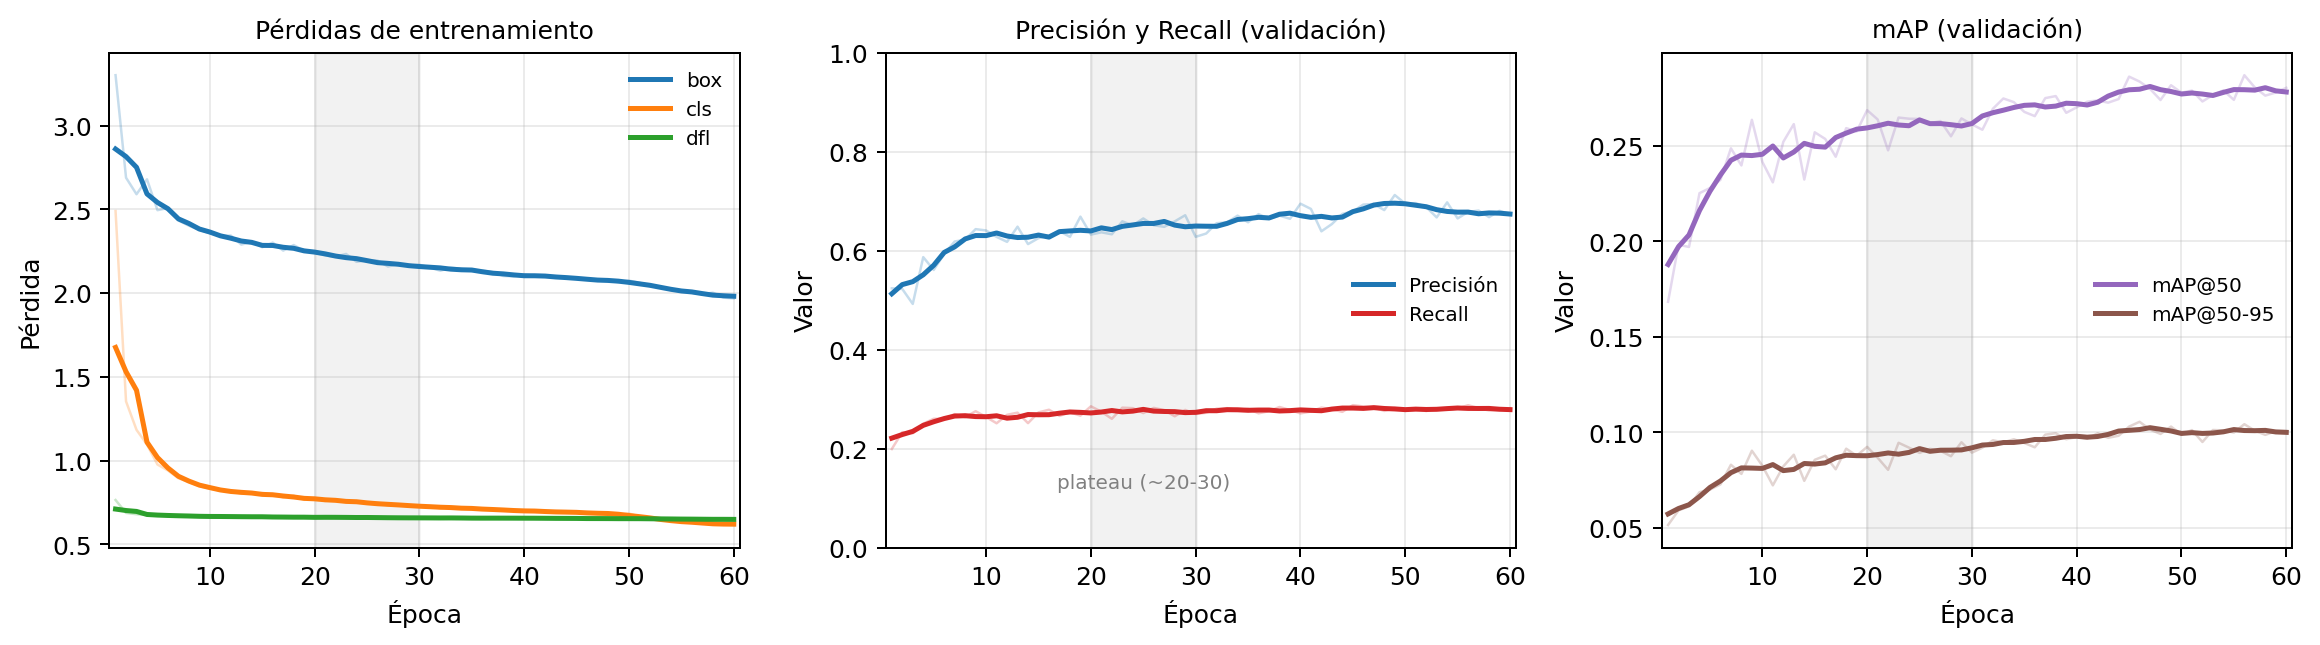
\includegraphics[width=\textwidth]{figuras/resultados/yolo_run02_curvas.png}
    \caption{Evolución del entrenamiento del detector YOLOv8n a lo largo de las \num{60}~épocas (tanda~2), resumida en tres paneles. Izquierda: las tres pérdidas de entrenamiento (box, cls, dfl) descienden de forma continua. Centro: la precisión y el recall de validación se estabilizan en una meseta aproximadamente entre las épocas 20 y 30 (banda sombreada). Derecha: el mAP@50 y el mAP@50-95 de validación siguen el mismo patrón; las épocas adicionales aportan una leve mejora de la precisión geométrica de las cajas (mAP@50-95) sin aumentar de forma significativa la cobertura (recall, mAP@50). En cada panel la línea tenue son los valores por época y la gruesa la tendencia suavizada.}
    \label{fig:yolo_run02_results}
\end{figure}

Las curvas muestran un comportamiento saludable: las pérdidas de entrenamiento descienden de forma continua y no hay señales de sobreajuste severo. Las métricas de validación se estabilizan entre las épocas~20 y~30 sin tendencia creciente clara a partir de ese punto. Esto indica que el límite del experimento no reside en la duración del entrenamiento, sino en la dificultad intrínseca del problema --- tamaño de las ráfagas en el espectrograma y ruido en el etiquetado automático ---, que las épocas adicionales no pueden superar.

\paragraph{Comparativa entre tandas.}

La \cref{tab:comparativa_epochs} compara los resultados de test de ambas tandas de entrenamiento.

\begin{table}[htbp]
\centering
\caption{Comparativa de resultados sobre el conjunto de prueba entre la tanda de \num{15}~épocas y la de \num{60}~épocas.}
\label{tab:comparativa_epochs}
\begin{tabular}{lccc}
\toprule
\textbf{Métrica} & \textbf{15 épocas} & \textbf{60 épocas} & \textbf{Diferencia} \\
\midrule
Precisión global        & 0,748 & 0,760 & +0,012 \\
Recall global           & 0,395 & 0,391 & $-$0,004 \\
mAP@50 global           & 0,386 & 0,388 & +0,002 \\
mAP@50-95 global        & 0,195 & 0,203 & +0,008 \\
mAP@50 drone            & 0,571 & 0,575 & +0,004 \\
mAP@50-95 drone         & 0,333 & 0,348 & +0,015 \\
mAP@50 interference     & 0,201 & 0,201 & $\pm$0,000 \\
mAP@50-95 interference  & 0,056 & 0,058 & +0,002 \\
\bottomrule
\end{tabular}
\end{table}

La tanda de \num{60}~épocas aporta una mejora marginal en la mayoría de métricas, siendo más apreciable en mAP@50-95 para \emph{drone} (+0,015). Esto es coherente con las curvas de la \cref{fig:yolo_run02_results}: las épocas adicionales refinan la localización geométrica de las cajas de dron sin aumentar el número de ráfagas detectadas.

\FloatBarrier
\paragraph{Separabilidad entre clases: matriz de confusión.}

La matriz de confusión normalizada constituye el resultado más relevante del experimento para responder a P2. En la matriz, las filas corresponden a las clases reales y las columnas a las clases predichas (incluyendo \emph{background}). Los valores de la diagonal indican la tasa de acierto de cada clase; los valores fuera de la diagonal entre dos clases activas indican confusión cruzada entre ellas; los valores en la columna \emph{background} indican ráfagas reales no detectadas.

\begin{figure}[htbp]
    \centering
    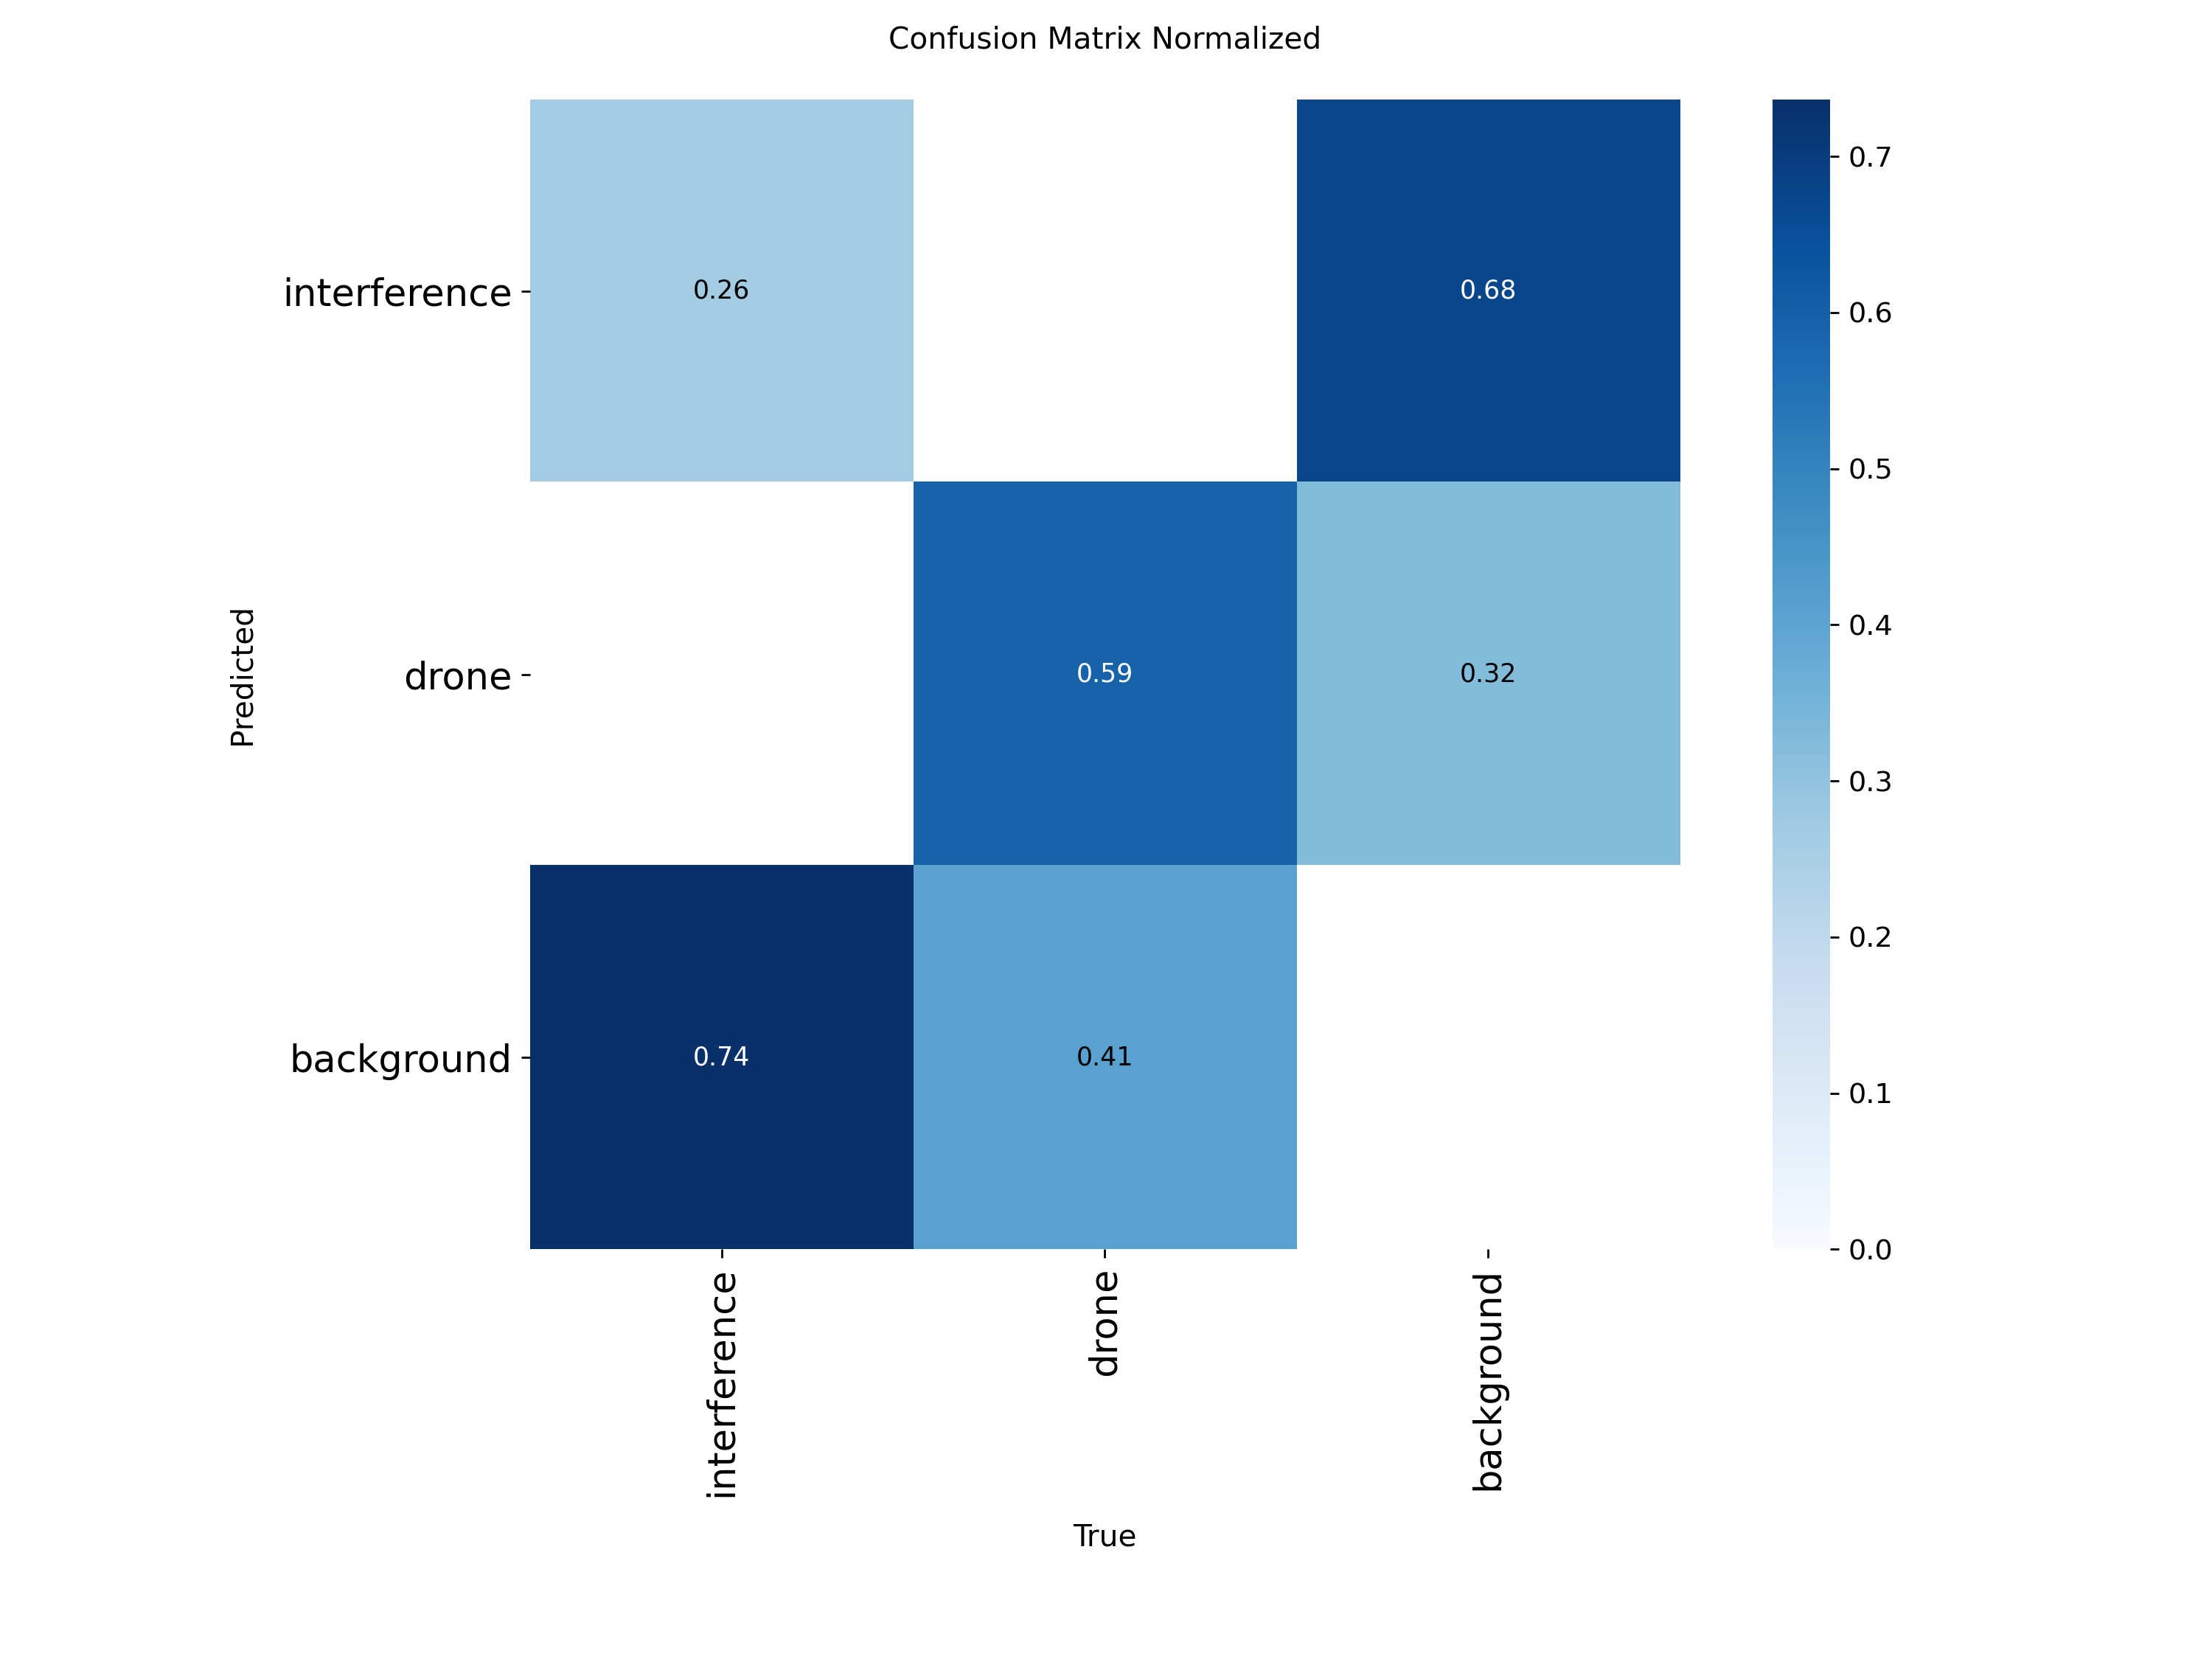
\includegraphics[width=0.75\textwidth]{figuras/resultados/confusion_matrix_normalized.png}
    \caption{Matriz de confusión normalizada del detector YOLOv8n sobre el conjunto de prueba. No se observa confusión cruzada entre \emph{drone} e \emph{interference}: cuando el modelo emite una predicción positiva, la clase asignada es correcta. Los errores son íntegramente falsos negativos (ráfagas reales asignadas a \emph{background}).}
    \label{fig:confusion_matrix_normalized}
\end{figure}

La \cref{fig:confusion_matrix_normalized} revela el resultado central del experimento: no existe confusión cruzada entre \emph{drone} e \emph{interference}. Ninguna ráfaga real de OcuSync es clasificada como interferencia, y ninguna ráfaga de interferencia es clasificada como señal de dron. Las tasas de confusión cruzada son ambas 0,00. Los errores son íntegramente falsos negativos: la tasa de detección a nivel de caja es de 0,42 para \emph{drone} y de 0,18 para \emph{interference}, con el complemento asignado a \emph{background}.

\FloatBarrier
\paragraph{Curvas precisión-recall y F1-confianza.}

La \cref{fig:box_pr_curve} muestra la curva precisión-recall del detector para ambas clases. La curva resume el equilibrio entre precisión y recall al variar el umbral de confianza: a umbrales altos el modelo es más selectivo (mayor precisión, menor recall); a umbrales bajos acepta más detecciones (mayor recall, menor precisión).

\begin{figure}[htbp]
    \centering
    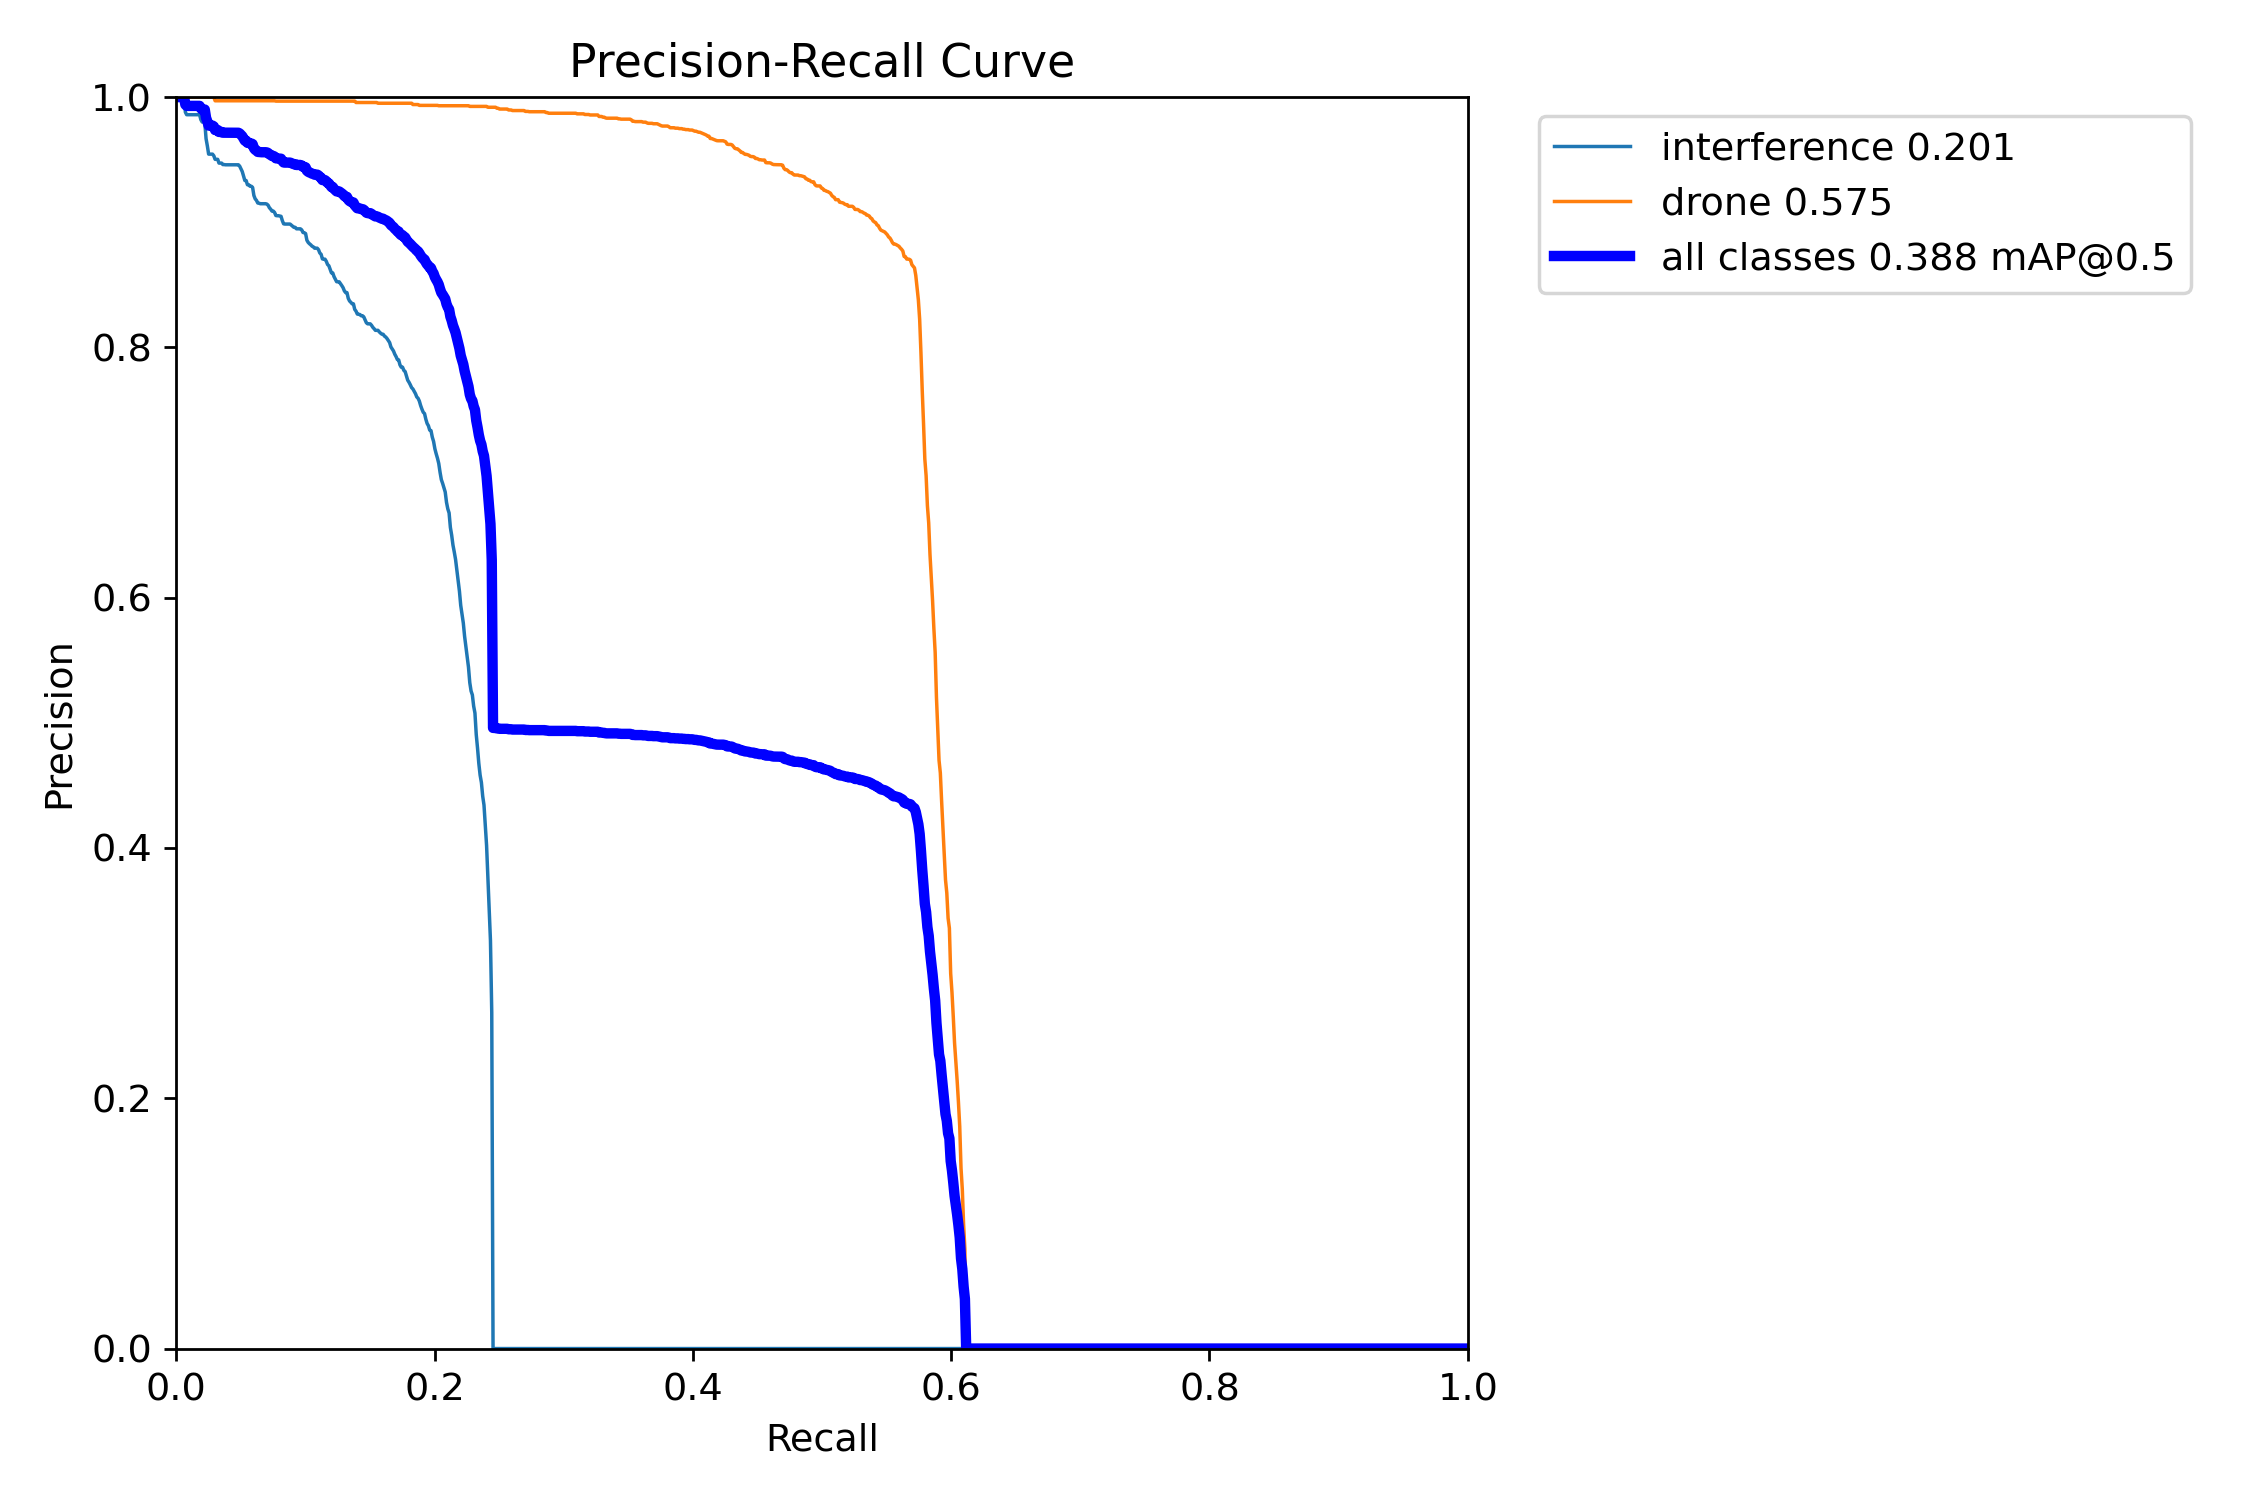
\includegraphics[width=0.85\textwidth]{figuras/resultados/BoxPR_curve.png}
    \caption{Curva precisión-recall del detector YOLOv8n sobre el conjunto de prueba. Cada punto corresponde a un umbral de confianza distinto. La clase \emph{drone} mantiene una precisión elevada en un rango de recall más amplio que \emph{interference}, lo que refleja la mayor homogeneidad de las ráfagas OcuSync respecto a las interferencias heterogéneas.}
    \label{fig:box_pr_curve}
\end{figure}

La \cref{fig:box_f1_curve} complementa la anterior mostrando el F1 en función del umbral de confianza. Esta curva permite identificar directamente el umbral que maximiza el F1 para cada clase o para el sistema global, y es la herramienta principal para seleccionar el punto de operación del sistema de detección. El máximo global se alcanza con umbrales de confianza bajos (en torno a 0,10-0,20), lo que indica que el detector asigna puntuaciones moderadas a una fracción relevante de ráfagas reales. En el experimento P3 se explotan explícitamente distintos valores de este umbral para determinar el punto de operación del clasificador de presencia.

\begin{figure}[htbp]
    \centering
    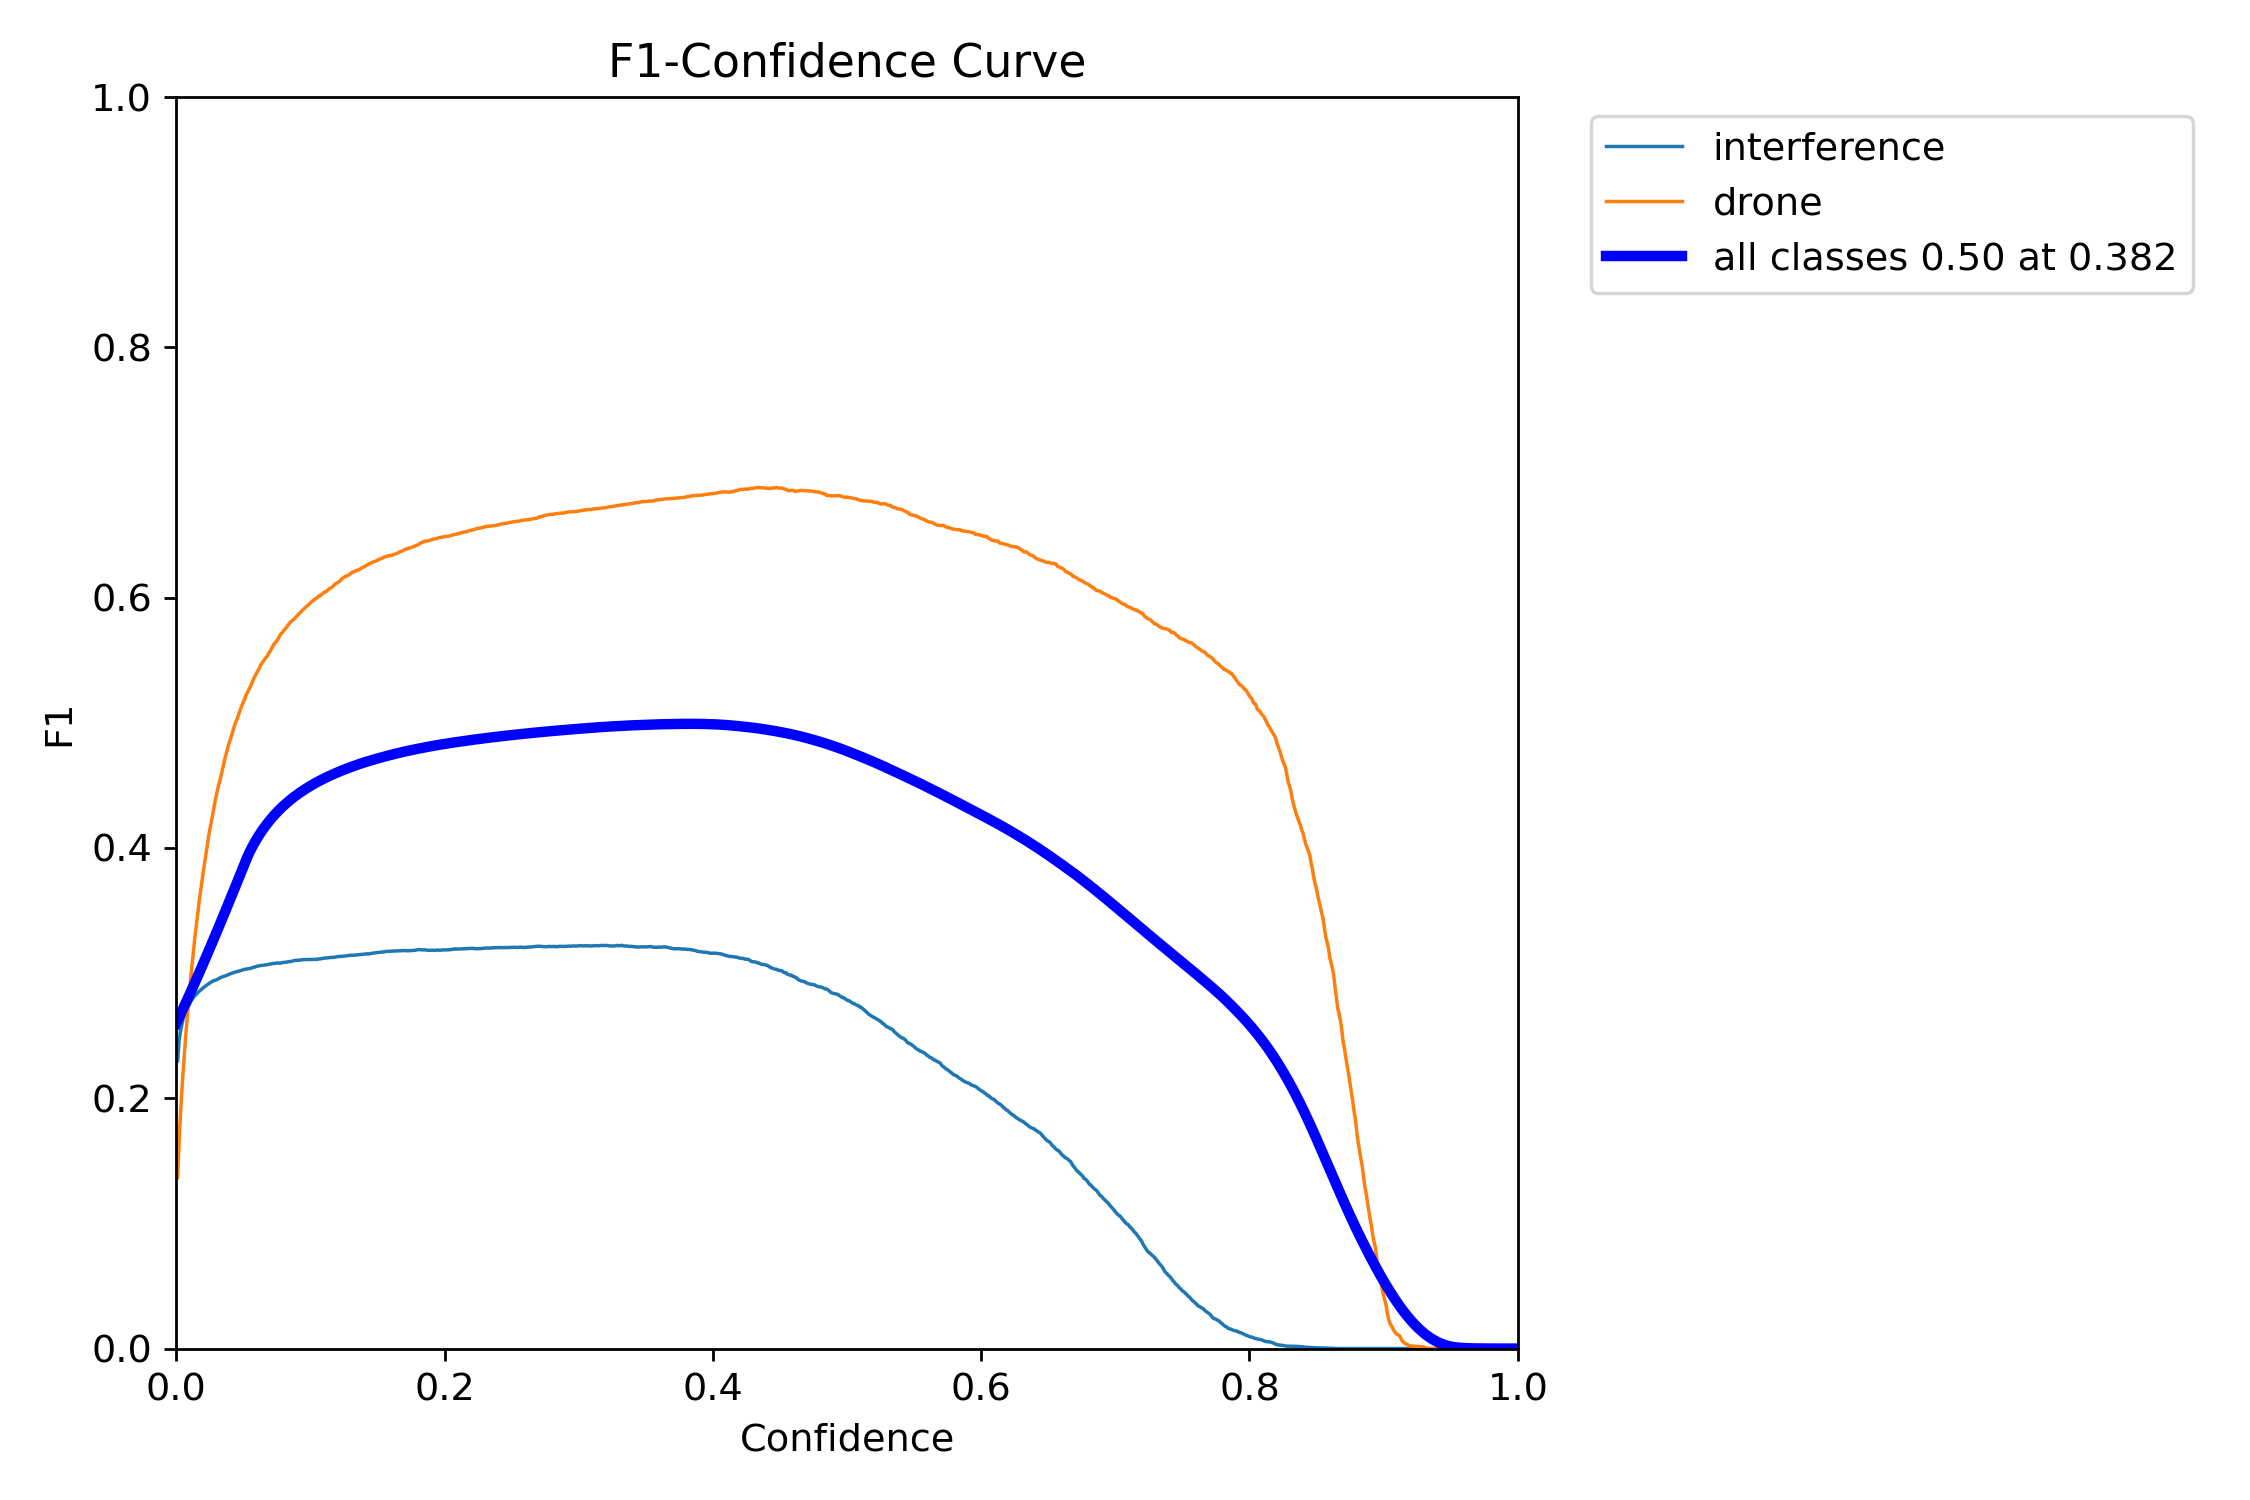
\includegraphics[width=0.85\textwidth]{figuras/resultados/BoxF1_curve.png}
    \caption{Curva F1-confianza del detector YOLOv8n. El eje horizontal representa el umbral de confianza mínimo para retener una detección, y el eje vertical el F1 resultante. El máximo global se alcanza con un umbral bajo, lo que indica que bajar el umbral recupera ráfagas reales sin penalizar excesivamente la precisión.}
    \label{fig:box_f1_curve}
\end{figure}

\FloatBarrier
\paragraph{Ejemplos cualitativos.}

Las \cref{fig:val_labels,fig:val_pred} comparan las etiquetas de referencia con las predicciones del modelo sobre un mismo lote de validación, permitiendo verificar visualmente la coherencia entre las métricas agregadas y el comportamiento sobre espectrogramas concretos.

\begin{figure}[htbp]
    \centering
    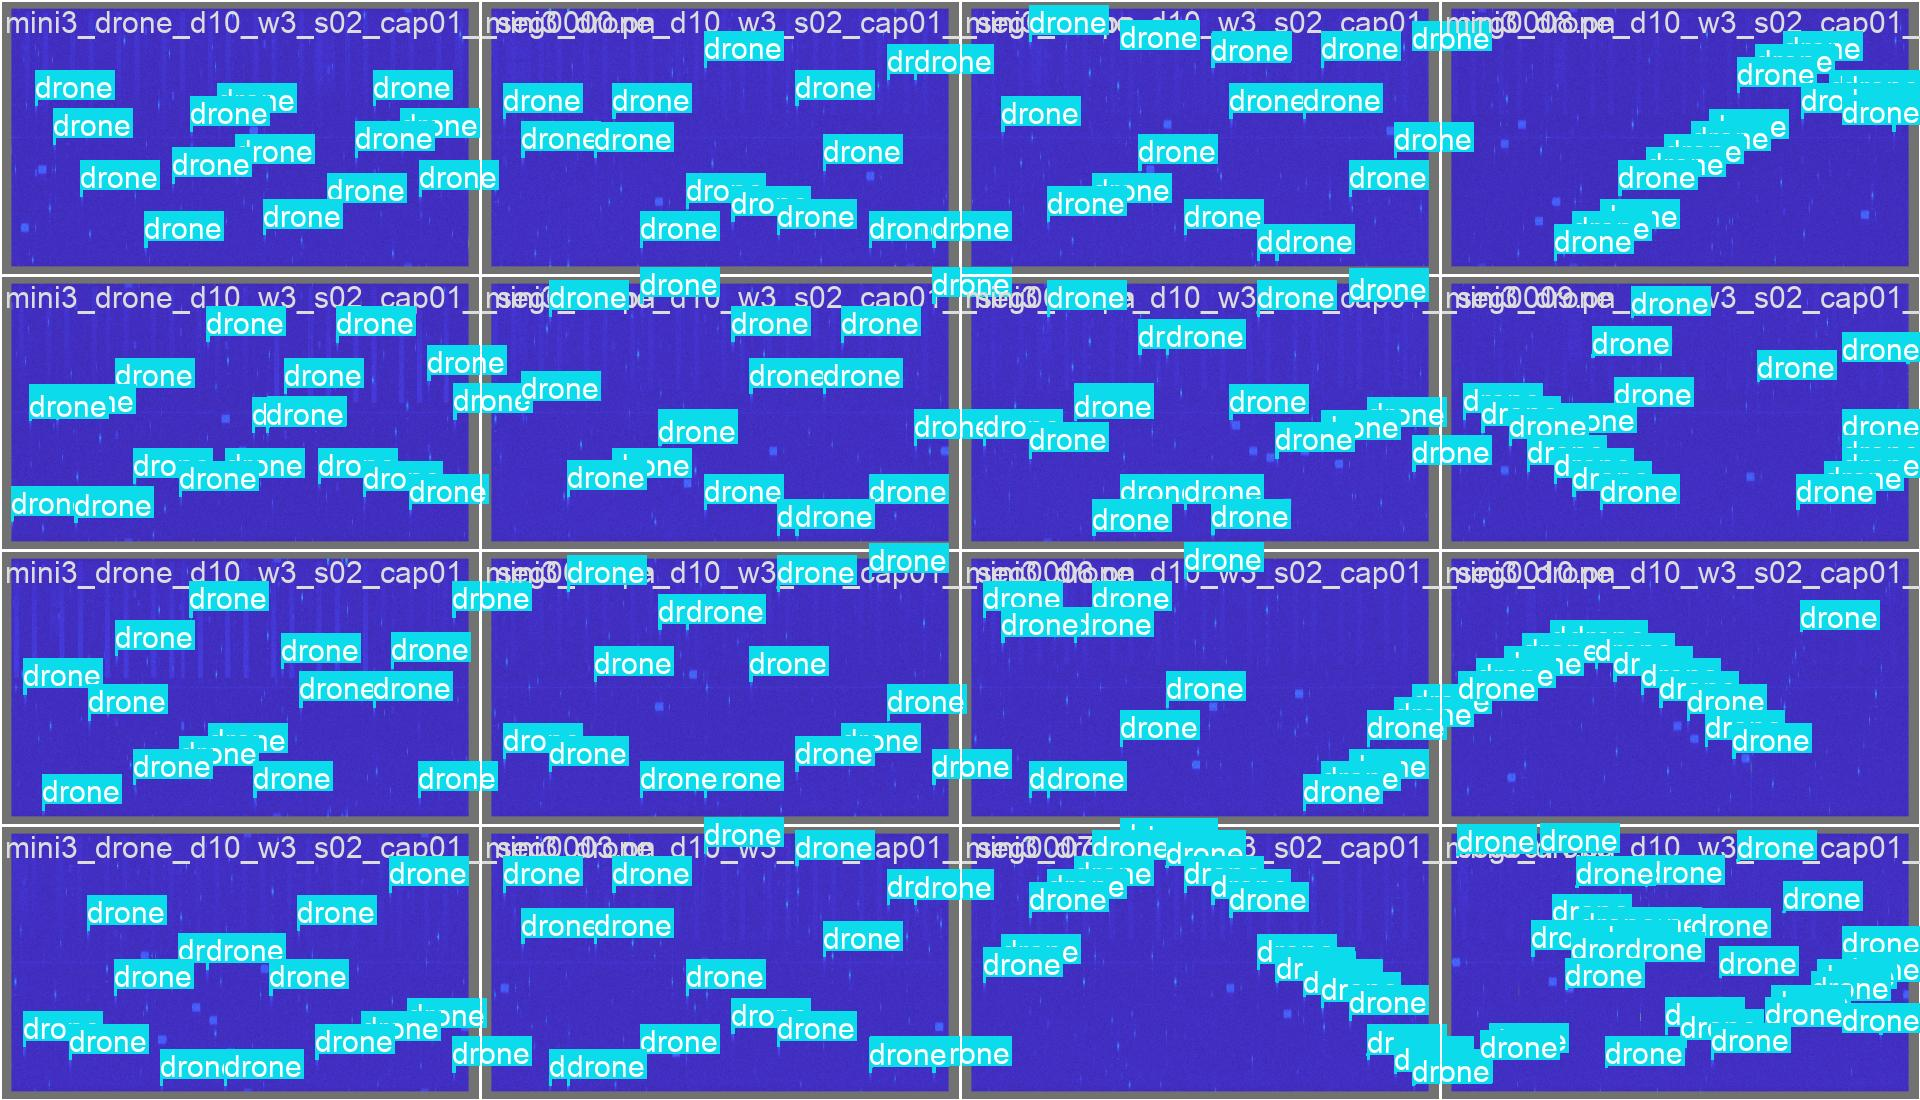
\includegraphics[width=0.9\textwidth]{figuras/resultados/val_batch0_labels.jpg}
    \caption{Etiquetas de referencia (\emph{ground truth}) sobre un lote de validación de capturas de dron. Cada caja delimita una ráfaga FHSS de OcuSync generada por el auto-etiquetado.}
    \label{fig:val_labels}
\end{figure}

\begin{figure}[htbp]
    \centering
    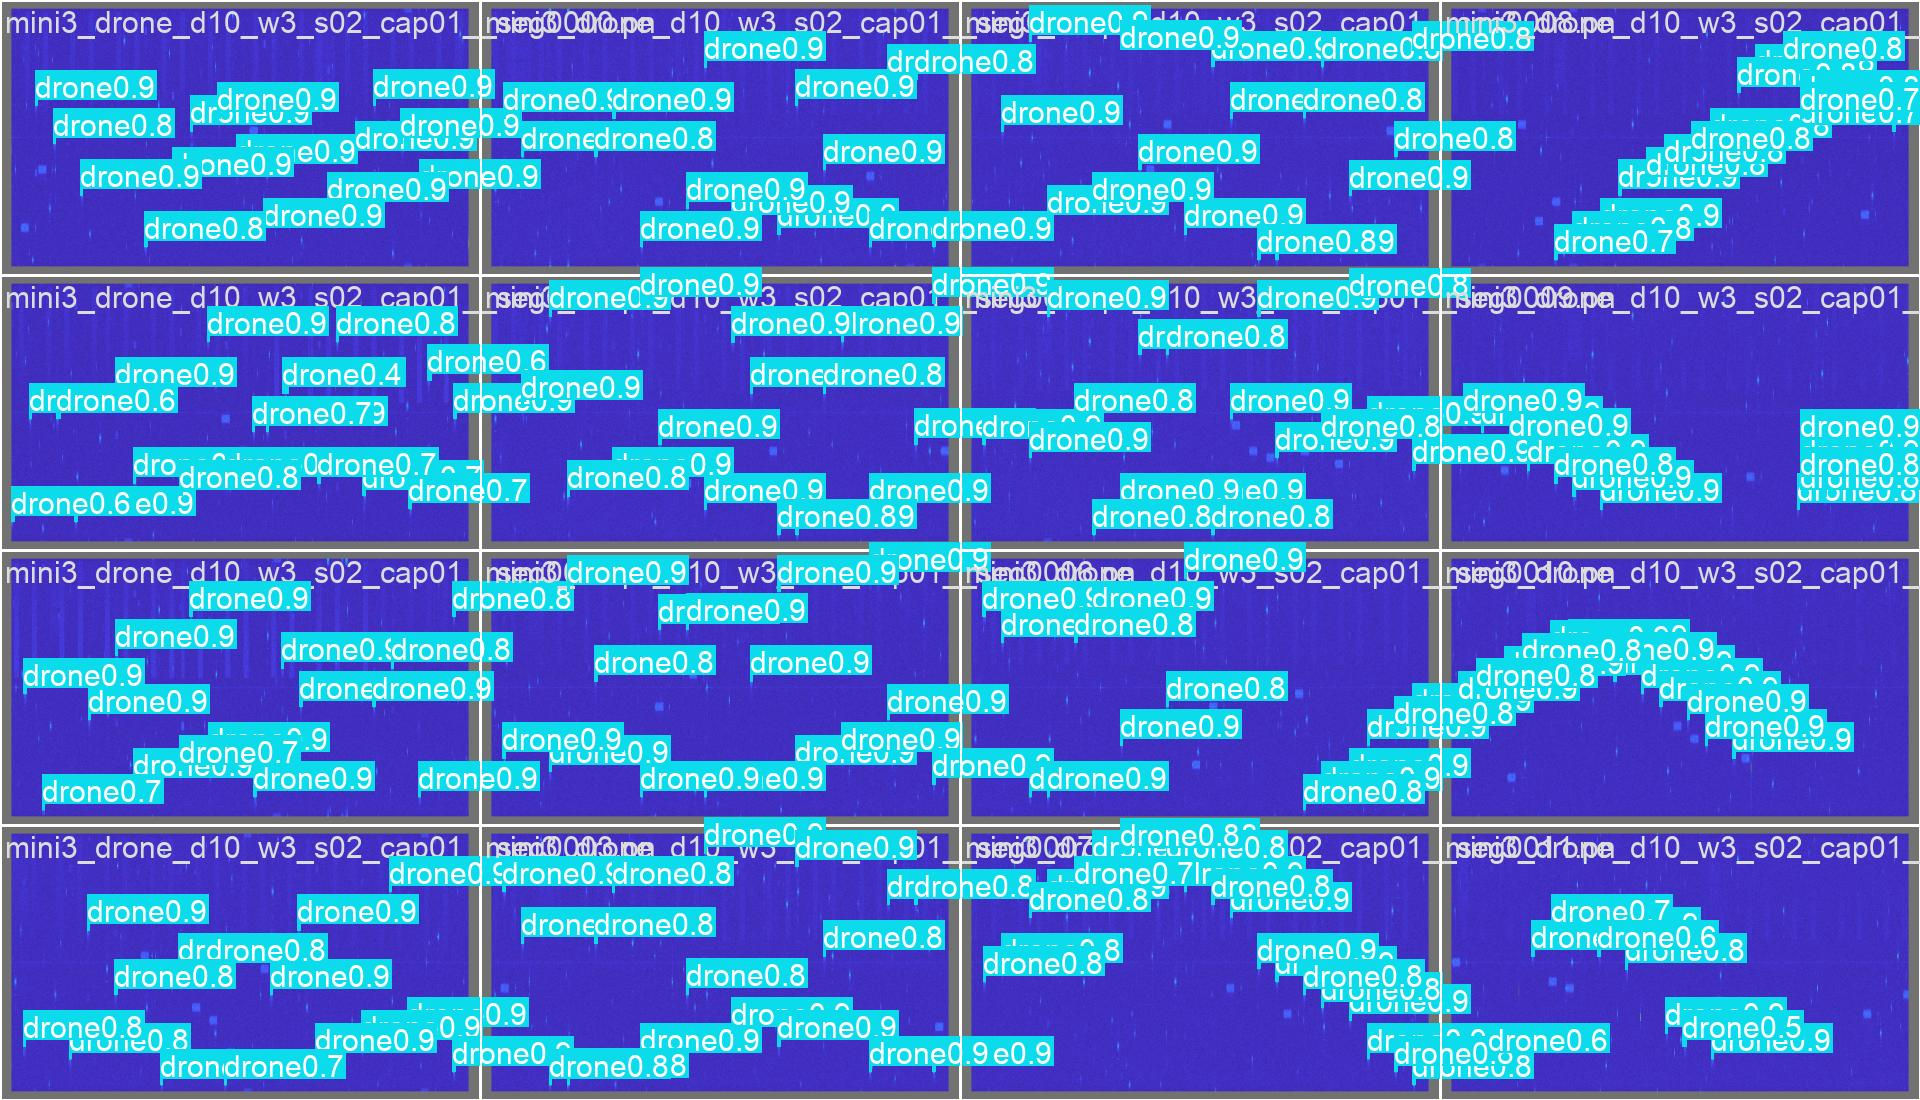
\includegraphics[width=0.9\textwidth]{figuras/resultados/val_batch0_pred.jpg}
    \caption{Predicciones del detector YOLOv8n sobre el mismo lote, con su puntuación de confianza asociada. Las cajas predichas se superponen sobre las mismas ráfagas FHSS que indican las etiquetas de referencia de la \cref{fig:val_labels}, con confianzas típicas entre 0,6 y 0,9. No aparecen cajas sobre regiones de fondo vacío: no hay falsos positivos.}
    \label{fig:val_pred}
\end{figure}

La comparación entre ambas figuras muestra que las cajas predichas se sitúan sobre las mismas ráfagas que las etiquetas de referencia. La densidad de cajas predichas es inferior a la de referencia, lo que es coherente con el recall de 0,39: el modelo no recupera todas las ráfagas etiquetadas. No aparecen, en cambio, cajas sobre regiones del espectrograma sin señal: no hay falsos positivos.

\FloatBarrier
\subsection{Interpretabilidad mediante EigenCAM}
\label{sec:eigencam}

Las métricas anteriores cuantifican el rendimiento del detector pero no revelan en qué características del espectrograma se apoya para inferir sus decisiones. Esta información es relevante para la auditabilidad del sistema: en aplicaciones de vigilancia, un detector debe poder justificar sus predicciones de forma verificable. Con este objetivo se aplica EigenCAM para analizar qué regiones del espectrograma activan internamente la red.

EigenCAM extrae las activaciones de la capa del cuello de YOLOv8 responsable de detectar objetos de tamaño pequeño y calcula su primera componente principal, produciendo un mapa de calor sobre el espectrograma. Al operar directamente sobre activaciones --- y no sobre gradientes respecto a ninguna clase objetivo ---, el mapa refleja las regiones que generan respuestas fuertes y coherentes en la red con independencia de la clase predicha.

\begin{figure}[htbp]
    \centering
    \begin{subfigure}[b]{0.48\textwidth}
        \centering
        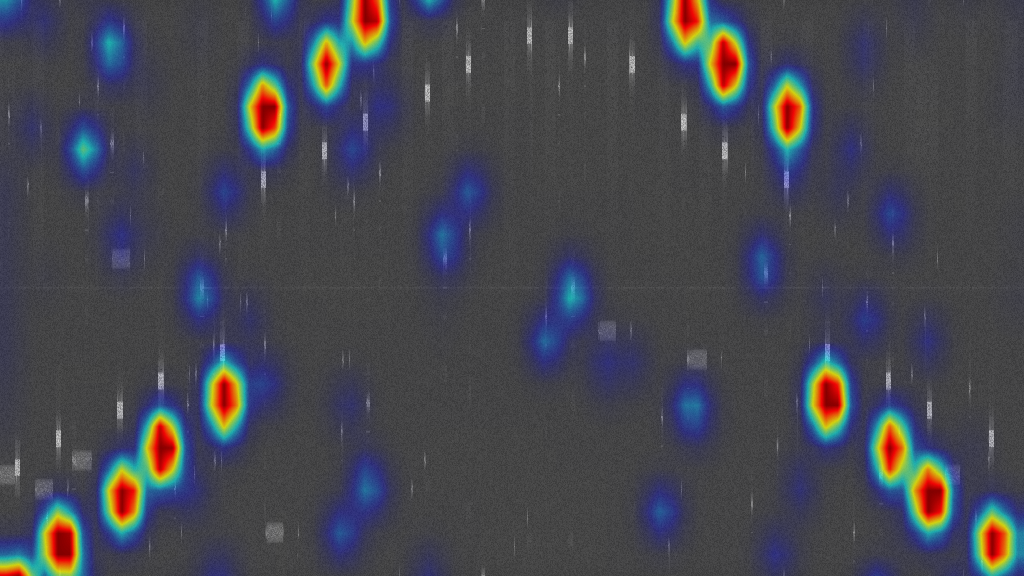
\includegraphics[width=\textwidth]{figuras/resultados/cam_drone_00.png}
        \caption{Captura con dron (protocolo OcuSync).}
        \label{fig:eigencam_drone}
    \end{subfigure}
    \hfill
    \begin{subfigure}[b]{0.48\textwidth}
        \centering
        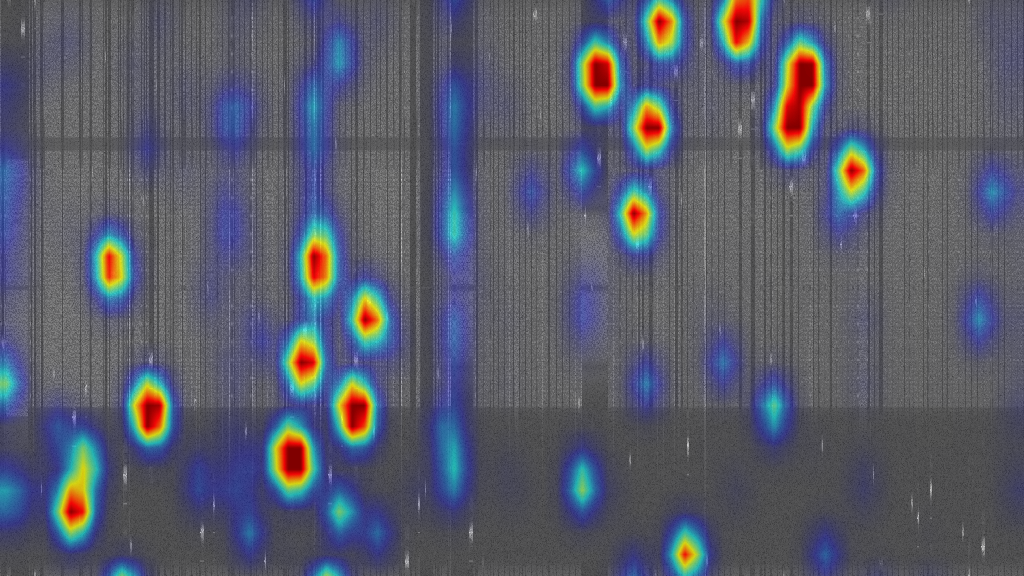
\includegraphics[width=\textwidth]{figuras/resultados/eigencam_interference.png}
        \caption{Captura de interferencia (WiFi/Bluetooth).}
        \label{fig:eigencam_interference}
    \end{subfigure}
    \caption{Mapas de saliencia EigenCAM del detector YOLOv8n sobre dos espectrogramas de prueba. El espectrograma subyacente se muestra en escala de grises y el color indica la intensidad de activación (rojo = alta, azul = baja). En la captura de dron, los focos de activación coinciden con las posiciones de las ráfagas OcuSync que las etiquetas de referencia de la \cref{fig:val_labels} delimitan como \emph{drone}. En la captura de interferencia, la activación recae sobre las estructuras WiFi y Bluetooth activas.}
    \label{fig:eigencam}
\end{figure}

La \cref{fig:eigencam} muestra los resultados para dos espectrogramas representativos del conjunto de prueba. En la captura de dron (\cref{fig:eigencam_drone}), los focos de calor son estructuras compactas que coinciden espacialmente con las ráfagas FHSS de OcuSync: las mismas posiciones que las etiquetas de referencia de la \cref{fig:val_labels} identifican como \emph{drone}. En la captura de interferencia (\cref{fig:eigencam_interference}), la activación recae sobre las columnas WiFi y las ráfagas Bluetooth. En ningún caso se producen activaciones sobre regiones de fondo vacío, lo que confirma que las respuestas de la red se asocian a estructuras de señal y no a artefactos del contexto de captura.

\FloatBarrier
Cabe señalar que EigenCAM no discrimina entre clases: el mapa indica únicamente dónde existen activaciones fuertes, no si estas corresponden a \emph{drone} o a \emph{interference}. La capacidad de separar ambas clases se sustenta en la ausencia de confusión cruzada de la \cref{fig:confusion_matrix_normalized}, y se refuerza cuantitativamente con el experimento de robustez de la \cref{sec:bloque_clasificacion}.
\subsection{Discusión}
\label{sec:p2_discusion}

El resultado central de P2 es la ausencia total de confusión cruzada entre \emph{drone} e \emph{interference}: cuando el detector emite una predicción positiva, la clase asignada es correcta. Esto responde afirmativamente a la pregunta de investigación P2: la firma FHSS del protocolo OcuSync es morfológicamente distinguible de los saltos Bluetooth y las tramas WiFi residuales cuando se analiza a nivel de región local en el espectrograma.

La diferencia de rendimiento entre las dos clases activas --- mAP@50 de 0,575 para \emph{drone} frente a 0,201 para \emph{interference} --- es coherente con la naturaleza del problema. La clase \emph{drone} agrupa señales de una fuente homogénea: ráfagas OcuSync de un único modelo, con parámetros de salto constantes. La clase \emph{interference} reúne señales heterogéneas --- saltos Bluetooth Classic, tramas WiFi residuales, ruido espurio --- cuya morfología varía considerablemente entre capturas, lo que dificulta aprender una representación compacta con la misma cantidad de datos.

\paragraph{La perspectiva correcta para el recall.}
El recall global de caja de 0,391 podría parecer, a primera vista, un rendimiento insuficiente para un sistema de vigilancia. Sin embargo, esta cifra mide la capacidad del detector de localizar cada ráfaga individual con precisión geométrica, usando un criterio de solapamiento IoU. Ese es el criterio correcto para auditar la calidad del detector como detector de objetos, pero no responde a la pregunta operativa del TFG: \emph{¿dado un espectrograma de \SI{0,1}{\second}, confirma el sistema si hay un dron emitiendo?}

Bajo esa óptica, la unidad de análisis relevante no es la caja individual sino la imagen completa. Una imagen típica de captura con dron activo contiene decenas de ráfagas en una sola ventana de \SI{0,1}{\second}, consecuencia directa del comportamiento del dron, que salta de canal decenas de veces por segundo. Con esa densidad de ráfagas, confirmar la presencia del dron --- es decir, detectar al menos $K$ de ellas --- es un problema estadísticamente mucho más sencillo que detectarlas todas: basta con que el modelo acierte en cualquiera de los múltiples intentos que ofrece la misma imagen. Un detector con recall individual de 0,39 que observe 60 ráfagas en una imagen esperaría detectar en torno a 23; la probabilidad de que ninguna de ellas supere el umbral $K=3$ es negligible.

\paragraph{Del recall de caja al recall de presencia.}
Esta propiedad --- que la redundancia temporal del protocolo OcuSync convierte un recall de caja modesto en un recall de presencia elevado --- se cuantifica rigurosamente en el experimento P3 de la \cref{sec:bloque_presencia}. Adelantamos aquí la conclusión: con el punto de operación recomendado ($\mathit{thr}=0{,}10$, $K=3$), el sistema confirma la presencia del dron en el \SI{91}{\percent} de las ventanas con dron activo, manteniendo una precisión y especificidad de \num{1,000} sobre las \num{300} imágenes de interferencia pura del test set --- cero falsas alarmas en todas las configuraciones evaluadas. El salto del \SI{39}{\percent} de recall de caja al \SI{91}{\percent} de recall de presencia no es un ajuste estadístico ni una concesión metodológica: es la consecuencia directa de que el protocolo OcuSync genera, por diseño, evidencia reiterada en cada ventana de tiempo.

\paragraph{Causas del recall de caja limitado.}
Aun siendo secundaria para la evaluación operativa, es importante entender la raíz del recall de caja de 0,391 para situar correctamente las limitaciones del experimento. Tres factores se acumulan. Primero, YOLOv8n es el modelo más ligero de la familia, con \num{3} millones de parámetros; tras el redimensionado de \num{1024}$\times$\num{576} a \num{640}$\times$\num{640}~píxeles, las ráfagas FHSS quedan reducidas a regiones de dos o tres píxeles de alto, que están en el límite de resolución de cualquier detector de objetos de una sola etapa. Segundo, el etiquetado automático introduce ruido sistemático en el \emph{ground truth}: las cajas se generan por umbral de energía, no por anotación humana, de modo que algunas ráfagas reales quedan sin etiquetar o con cajas que no delimitan con precisión la extensión temporal de la señal; cualquier predicción que no solape suficientemente con esa referencia imperfecta queda penalizada como falso negativo aunque la detección sea semánticamente correcta. Tercero, el dataset v3 es de interior con una configuración de ganancia fija; la variedad de condiciones de propagación es limitada, y es esperable que un conjunto de datos con mayor diversidad de escenarios y distancias mejore el recall.

Ninguno de estos tres factores es un límite del problema: son límites del experimento concreto, documentados como líneas de trabajo futuro. El resultado fundamental --- cero confusión cruzada --- es independiente de ellos; se mantiene tanto en el run01 de 15 épocas como en el run02 de 60 épocas, lo que indica que la separabilidad morfológica está bien capturada por el modelo base.

\paragraph{Dirección de los falsos positivos.}
Un detalle operativamente relevante es el sesgo de las activaciones falsas del modelo. La matriz de confusión de la \cref{fig:confusion_matrix_normalized} muestra que el 82\,\% de las predicciones positivas sobre regiones sin señal real se clasifican como \emph{drone}, frente al 18\,\% que se clasifican como \emph{interference}. Para una aplicación de detección de drones, este sesgo es preferible al opuesto: una alarma adicional innecesaria es un coste operativo menor y asumible, mientras que la omisión de una amenaza real tiene consecuencias más graves. El modelo falla hacia el lado seguro.

En definitiva, el Stage~1 no es un detector de ráfagas individuales de alta precisión geométrica, sino un mecanismo de evidencia acumulada que aprovecha la redundancia temporal del protocolo OcuSync para confirmar la presencia de la señal con robustez operativa. La evaluación adecuada no es el recall de caja sino la capacidad de decidir correctamente sobre presencia, que el experimento P3 cuantifica de forma rigurosa.

% =============================================================================
% P3 --- version revisada (tono TFG). Mantiene el barrido thr x K y el mapa de
% calor como unica figura. Se eliminan presencia_por_captura,
% yolo_rafagas_por_imagen y la matriz de confusion 2x2.
% Figura: presencia_heatmap.png
% =============================================================================
\section{P3 --- ¿Puede el sistema confirmar operativamente la presencia de un dron?}
\label{sec:bloque_presencia}

\subsection{Planteamiento del experimento}
\label{sec:p3_planteamiento}

El recall de caja del \SI{39}{\percent} obtenido en P2 podría sugerir que el sistema solo detecta una de cada tres ráfagas reales. Sin embargo, esa métrica responde a una pregunta de naturaleza distinta a la que plantea una aplicación de vigilancia. La cuestión operativa no es cuántas ráfagas individuales localiza el detector en una imagen, sino si el sistema decide correctamente, para cada ventana de \SI{0.1}{\second}, la presencia o ausencia de un dron en la escena.


Para abordarla se introduce un \emph{clasificador de presencia} a nivel de imagen, definido formalmente en la \cref{sec:implementacion_presencia}: una ventana se declara positiva cuando el número de cajas de clase \emph{drone} con confianza mayor o igual que un umbral $\mathit{thr}$ alcanza al menos un mínimo de~$K$ ráfagas. Esta formulación introduce dos grados de libertad ---el umbral de confianza $\mathit{thr}$ y el número mínimo de ráfagas $K$--- cuyo efecto conjunto sobre el rendimiento se evalúa mediante un barrido sistemático. Se exploran cuatro umbrales de confianza, $\mathit{thr} \in \{0{,}10,\, 0{,}25,\, 0{,}40,\, 0{,}50\}$, y cuatro valores mínimos de ráfagas, $K \in \{1, 2, 3, 4\}$, lo que da lugar a \num{16}~configuraciones evaluadas sobre las \num{600}~imágenes del conjunto de prueba (\num{300} con dron y \num{300} sin dron, en balance exacto).

\subsection{Resultados}
\label{sec:p3_resultados}

La \cref{fig:presencia_heatmap} recoge el recall de presencia de las \num{16}~configuraciones. El resultado más destacable es transversal a todas ellas: la precisión y la especificidad valen exactamente \num{1,000} en las dieciséis combinaciones. Es decir, el sistema no declara la presencia de un dron en ninguna de las \num{300}~imágenes de interferencia pura, con independencia del umbral de confianza y del mínimo de ráfagas elegidos. La elección de $(\mathit{thr}, K)$ no introduce falsos positivos; únicamente regula la sensibilidad, esto es, el recall de presencia.


Estos valores se representan como un mapa de calor, que facilita la lectura del compromiso entre sensibilidad y exigencia: el recall de presencia es máximo en la esquina superior izquierda (umbral de confianza bajo y pocas ráfagas exigidas) y decrece de forma monótona al endurecer cualquiera de los dos parámetros.

\begin{figure}[htbp]
    \centering
    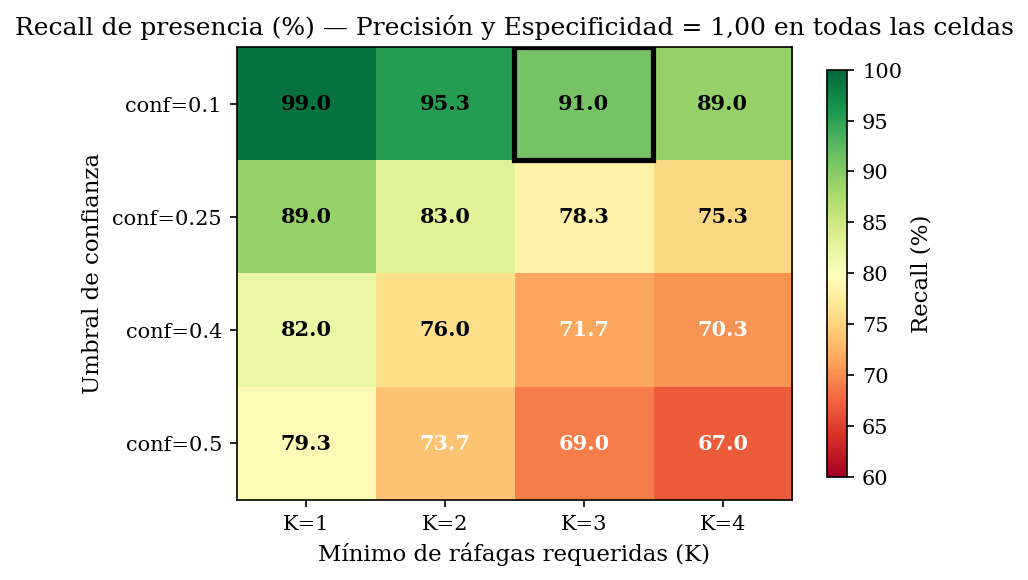
\includegraphics[width=0.70\textwidth]{figuras/resultados/presencia_heatmap.png}
    \caption{Mapa de calor del recall de presencia (\%) en función del umbral de confianza $\mathit{thr}$ y del mínimo de ráfagas~$K$. Las celdas más claras corresponden a mayor recall. El recuadro destacado marca el punto de operación recomendado ($\mathit{thr}=0{,}10$,\, $K=3$), con recall del \SI{91}{\percent} y F1\,=\,\num{0,953}. La precisión y la especificidad valen \num{1,000} en todas las celdas.}
    \label{fig:presencia_heatmap}
\end{figure}

\FloatBarrier
Como punto de operación se adopta $\mathit{thr}=0{,}10$,\, $K=3$, que maximiza el recall de presencia (\SI{91}{\percent}, F1\,=\,\num{0,953}) exigiendo a la vez la coincidencia de tres ráfagas independientes por ventana, lo que protege frente a detecciones espurias aisladas. En este punto, de las \num{300}~ventanas con dron el sistema confirma \num{273} y deja \num{27} sin confirmar (falsos negativos), mientras que las \num{300}~ventanas de interferencia pura se rechazan en su totalidad, sin una sola falsa alarma.


\subsection{Discusión}
\label{sec:p3_discusion}

El resultado central de P3 es la ausencia total de falsos positivos en las \num{16}~configuraciones evaluadas: el sistema no confirma la presencia de un dron en ningún espectrograma que contenga únicamente WiFi y Bluetooth, incluidas las capturas de interferencia más intensa. La precisión y la especificidad perfectas se mantienen con independencia de los parámetros del clasificador de presencia, lo que indica que la decisión positiva del sistema es altamente fiable.


La aparente paradoja entre el recall de caja (\SI{39}{\percent}) y el recall de presencia (\SI{91}{\percent}) se explica por la redundancia temporal del protocolo OcuSync. Una ventana con dron contiene decenas de ráfagas FHSS ---consecuencia directa de un esquema de salto que cambia de canal decenas de veces por cada \SI{0.1}{\second}---, de modo que, aunque el detector falle la mayoría de las ráfagas a nivel individual, le basta con acertar unas pocas para superar el mínimo de $K=3$. El clasificador de presencia actúa así como un agregador que convierte múltiples detecciones débiles en una decisión binaria robusta. En las ventanas sin dron, por el contrario, las detecciones espurias son tan escasas que nunca alcanzan ese mínimo, lo que sostiene la especificidad perfecta.


El análisis por captura matiza el origen de los \num{27}~falsos negativos: se concentran en la captura a \SI{5}{\meter} con WiFi limpio (nivel L1), mientras que la captura a \SI{10}{\meter} con WiFi saturado (nivel L3) se confirma en el \SI{100}{\percent} de sus ventanas. Este comportamiento, contraintuitivo a primera vista, admite una explicación coherente con el protocolo: ante una interferencia intensa, OcuSync tiende a incrementar la densidad de retransmisiones, lo que aumenta el número de ráfagas por ventana y facilita la confirmación de presencia. De ser correcta esta interpretación, el sistema operaría mejor precisamente en el escenario de despliegue más exigente.


Conviene encuadrar el alcance de estas cifras: el barrido se ha realizado sobre el conjunto de prueba del dataset~v3, de carácter interior y controlado (\cref{cap:implementacion}). La especificidad perfecta y el recall del \SI{91}{\percent} son sólidos dentro de ese dominio; su validación sobre un conjunto con mayor diversidad de distancias, niveles de interferencia y entornos ---el dataset~v4 propuesto en el \cref{cap:conclusiones}--- queda planteada como trabajo futuro. En cualquier caso, el punto de operación $\mathit{thr}=0{,}10$,\, $K=3$ constituye un compromiso razonable entre sensibilidad y robustez para una primera versión del sistema de vigilancia.


\section{P4 --- ¿Identifica el sistema el modelo de dron y discrimina por morfología o por intensidad?}
\label{sec:bloque_clasificacion}

Esta sección responde a dos preguntas relacionadas: si el clasificador ResNet18 puede identificar el modelo concreto de dron una vez confirmada la presencia, y si la discriminación aprendida se sustenta en la morfología espectro-temporal de las ráfagas o en el nivel medio de potencia. La primera evalúa la segunda etapa del \emph{pipeline}; la segunda cierra la hipótesis central del trabajo.

\subsection{Planteamiento del experimento}
\label{sec:p4_planteamiento}

\paragraph{Parte A --- Clasificación de modelos.}
El clasificador Stage~2, cuya arquitectura y configuración de entrenamiento se describen en la \cref{sec:implementacion_stage2}, distingue seis clases: cinco modelos de plataforma (\emph{f450}, \emph{hunter}, \emph{mavic\_video}, \emph{mavic\_novideo} y \emph{mini3}) más la clase \emph{interference}, a partir de capturas de campo abierto con drones reales. El conjunto de prueba contiene \num{941}~segmentos de \num{8}~capturas distintas, particionados por captura. El mejor modelo, seleccionado por macro-F1 sobre validación, corresponde a la época~\num{10} (macro-F1 de validación \num{0,959}).

El Mavic se separa en dos clases ---\emph{mavic\_video} y \emph{mavic\_novideo}--- porque durante la captura se recorrió todo el espectro en busca de la señal del dron. Esto dio lugar a dos tipos de región según el instante: tramos en los que el enlace transmitía vídeo (canal OFDM de banda ancha) y tramos en los que solo emitía la señal de control FHSS. Ambas condiciones presentan una morfología distinta en el espectrograma, por lo que se etiquetan como clases separadas.

\paragraph{Parte B --- Barrido de SNR.}
Para verificar si la clasificación se apoya en la morfología o en el nivel de energía se emplea el protocolo de barrido descrito en la \cref{sec:implementacion_snr}: se inyectan dos tipos de ruido (AWGN y FHSS sintético) a la misma potencia total en el dominio IQ, y se regenera el espectrograma con el mismo \emph{pipeline} de entrenamiento. El barrido cubre los niveles de SNR $\{+\infty,\, +20,\, +15,\, +10,\, +5,\, 0,\, -5,\, -10,\, -15,\, -20\}$~dB.

La hipótesis es que, si el clasificador discrimina por morfología --- por \emph{dónde} está la energía, no por \emph{cuánta} hay ---, el FHSS sintético (que concentra toda su potencia en el \SI{1,5}{\percent} del plano tiempo-frecuencia) debería degradar el rendimiento mucho menos que el AWGN (que distribuye esa misma potencia uniformemente por toda la imagen).

\subsection{Resultados de clasificación multiclase}
\label{sec:p4_clasificacion}

La \cref{fig:stage2_curvas} muestra la evolución de la pérdida y el macro-F1 del clasificador durante el entrenamiento. El \textbf{macro-F1} es la media aritmética del F1 de las seis clases, dando a cada una el mismo peso con independencia de su número de muestras; por ello penaliza con fuerza el fallo en una clase minoritaria, lo que lo convierte en una métrica exigente y adecuada para un conjunto desbalanceado como este.

\begin{figure}[htbp]
    \centering
    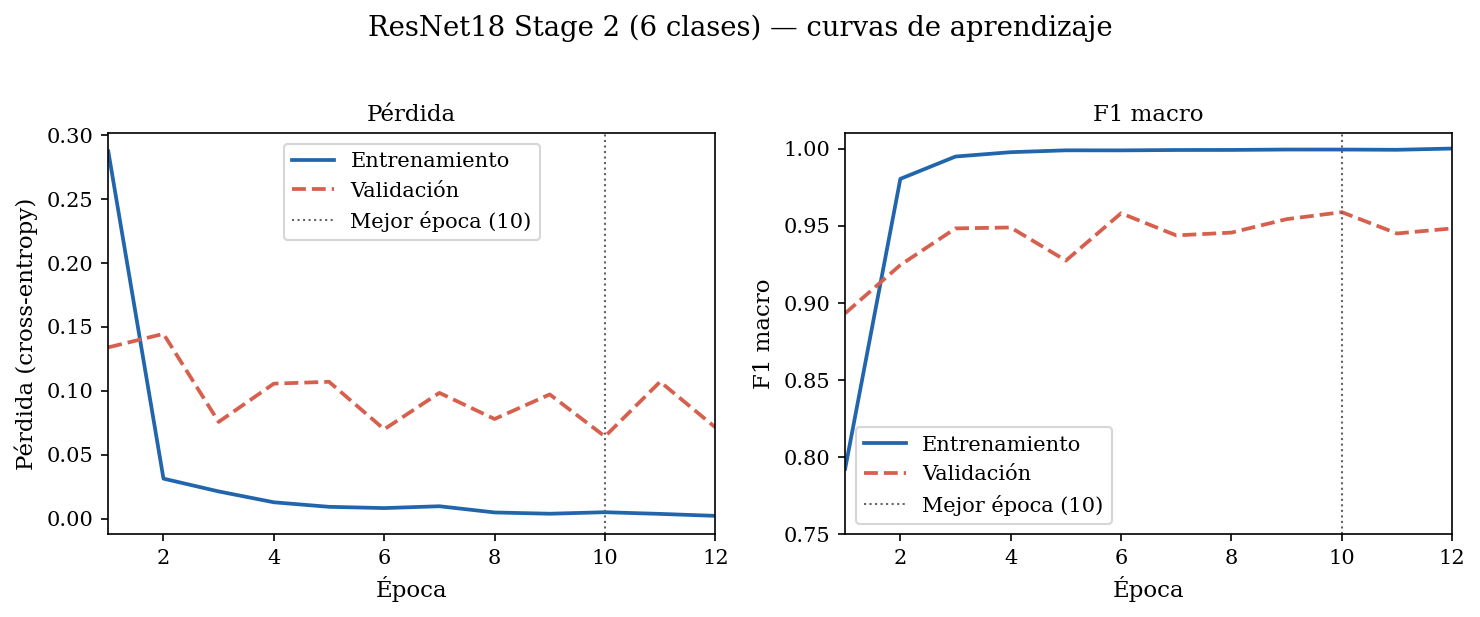
\includegraphics[width=0.85\textwidth]{figuras/resultados/stage2_curvas_aprendizaje.png}
    \caption{Evolución de la pérdida y el macro-F1 en entrenamiento y validación del clasificador ResNet18 de seis clases. El macro-F1 promedia el F1 de las seis clases con igual peso. La curva de entrenamiento asciende hacia F1\,=\,1,0, mientras que la de validación oscila entre \num{0,93} y \num{0,96}. Esta brecha indica sobreajuste moderado y justifica seleccionar el \emph{checkpoint} de mejor macro-F1 en validación en lugar de la última época.}
    \label{fig:stage2_curvas}
\end{figure}

Las curvas muestran un sobreajuste moderado: el F1 de entrenamiento sube hacia \num{1,0} mientras que el de validación oscila sin convergencia clara al final del entrenamiento. Esto justifica haber seleccionado el \emph{checkpoint} de la época~\num{10} por su máximo F1 de validación.
Los resultados globales sobre el conjunto de prueba se presentan en la \cref{tab:stage2_global}. El resultado más relevante para este TFG es que el DJI Mini~3 obtiene F1\,=\,\num{0,992} sobre \num{300}~muestras: prácticamente clasificación sin errores. Las clases \emph{mavic\_video} y \emph{f450} también se reconocen con alta fiabilidad.

\begin{table}[htbp]
\centering
\caption{Resultados globales del clasificador ResNet18 de seis clases sobre el conjunto de prueba (\num{941}~segmentos).}
\label{tab:stage2_global}
\begin{tabular}{lc}
\toprule
\textbf{Métrica} & \textbf{Valor} \\
\midrule
Exactitud       & 0,898 \\
F1~macro        & 0,764 \\
F1~ponderado    & 0,872 \\
Precisión macro & 0,730 \\
Recall macro    & 0,819 \\
\bottomrule
\end{tabular}
\end{table}

El desglose por clase de la \cref{tab:stage2_por_clase} localiza el origen del macro-F1 de \num{0,764}: está íntegramente condicionado por el rendimiento de una única clase.

\begin{table}[htbp]
\centering
\caption{Métricas por clase del clasificador ResNet18 de seis clases sobre el conjunto de prueba.}
\label{tab:stage2_por_clase}
\begin{tabular}{lcccc}
\toprule
\textbf{Clase}       & \textbf{Soporte} & \textbf{Precisión} & \textbf{Recall} & \textbf{F1} \\
\midrule
f450                 & 30               & 0,811              & 1,000           & 0,896 \\
hunter               & 120              & 0,588              & 1,000           & 0,741 \\
mavic\_video         & 120              & 1,000              & 1,000           & 1,000 \\
mavic\_novideo       & 71               & 0,000              & 0,000           & 0,000 \\
mini3                & 300              & 0,984              & 1,000           & 0,992 \\
interference         & 300              & 1,000              & 0,917           & 0,957 \\
\midrule
\textbf{Macro}       & 941              & 0,730              & 0,819           & 0,764 \\
\bottomrule
\end{tabular}
\end{table}

La \cref{fig:stage2_confusion} muestra la distribución de errores mediante la matriz de confusión normalizada. En esta representación las filas corresponden a las clases reales y las columnas a las predichas; los valores de la diagonal indican la proporción de muestras clasificadas correctamente para cada clase, y los valores fuera de la diagonal reflejan las confusiones entre clases.

\begin{figure}[htbp]
    \centering
    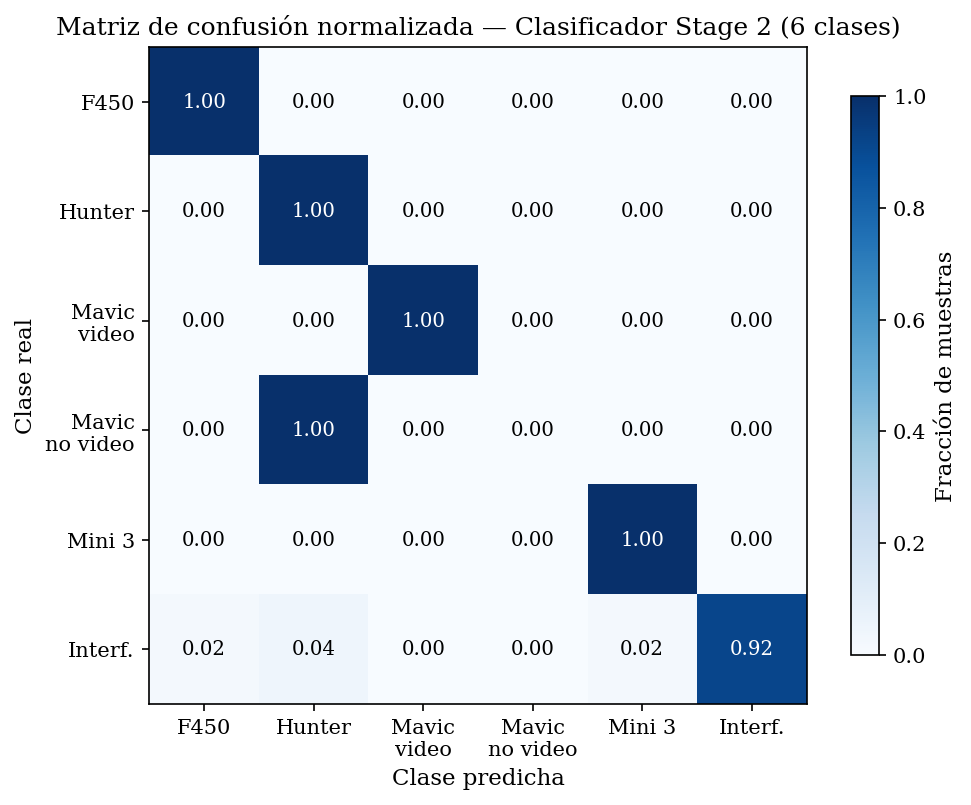
\includegraphics[width=0.75\textwidth]{figuras/resultados/stage2_confusion_matrix_norm.png}
    \caption{Matriz de confusión normalizada del clasificador ResNet18 de seis clases sobre el conjunto de prueba. La diagonal es prácticamente perfecta para cinco clases. La clase \emph{mavic\_novideo} colapsa íntegramente a \emph{hunter}, constituyendo el único fallo relevante del clasificador.}
    \label{fig:stage2_confusion}
\end{figure}




\begin{figure}[htbp]
    \centering
    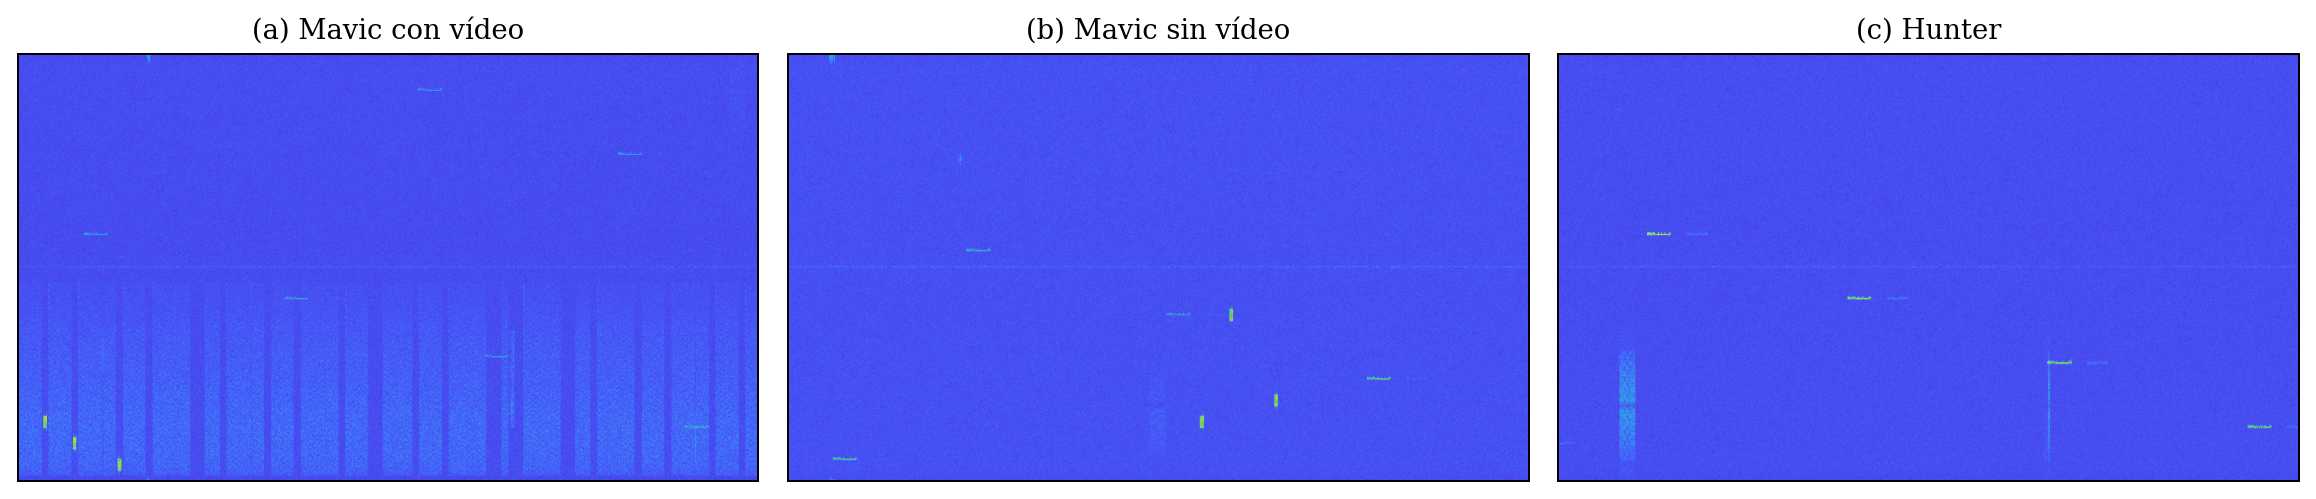
\includegraphics[width=\textwidth]{figuras/resultados/stage2_morfologia_mavic_hunter.png}
    \caption{Comparativa morfológica que explica la confusión entre \emph{mavic\_novideo} y \emph{hunter}. (a) Mavic con vídeo: el enlace emite el canal de banda ancha (OFDM) junto a la señal de control, produciendo bandas anchas y densas claramente distintivas. (b) Mavic sin vídeo: al desactivarse el vídeo, solo queda la señal de control FHSS, reducida a ráfagas dispersas. (c) Hunter: su emisión presenta el mismo aspecto de ráfagas dispersas. Los paneles (b) y (c) son morfológicamente casi indistinguibles, lo que justifica que el clasificador asigne las muestras de \emph{mavic\_novideo} a \emph{hunter}.}
    \label{fig:stage2_morfologia}
\end{figure}



El caso de \emph{mavic\_novideo} no es un fallo metodológico, sino una consecuencia directa de la morfología de la señal, ilustrada en la \cref{fig:stage2_morfologia}. Con el vídeo activo (\cref{fig:stage2_morfologia}a), el Mavic emite un canal OFDM de banda ancha que lo hace inconfundible. Al desactivar el vídeo (\cref{fig:stage2_morfologia}b), su emisión se reduce a la señal de control FHSS ---ráfagas dispersas--- cuya morfología coincide con la del Hunter (\cref{fig:stage2_morfologia}c). Sin el canal de vídeo no queda ningún rasgo espectral que separe ambas clases con los datos disponibles, por lo que el clasificador asigna la totalidad de las muestras de \emph{mavic\_novideo} a \emph{hunter}. Su resolución requeriría más capturas de esta clase en condiciones variadas, no un rediseño del sistema.








\subsection{Resultados del barrido de SNR}
\label{sec:resultados_snr}

La \cref{tab:snr_accuracy} presenta la exactitud del clasificador frente al SNR para ambos modelos de ruido. El control a SNR infinito reproduce exactamente la exactitud del test original (\num{0,898}), confirmando la fidelidad del \emph{pipeline} de inyección al proceso de entrenamiento.



Antes de cuantificar el efecto del ruido conviene observarlo directamente. La \cref{fig:snr_ejemplos} muestra un mismo espectrograma del DJI Mini~3 degradado por los dos modelos de ruido a distintos niveles de SNR: el AWGN (\cref{fig:snr_ejemplo_awgn}) enmascara la señal subiendo el fondo de forma uniforme, mientras que el FHSS sintético (\cref{fig:snr_ejemplo_fhss}) mantiene las ráfagas visibles porque concentra su energía en regiones puntuales. Este contraste anticipa el resultado cuantitativo que se presenta a continuación.



\begin{figure}[htbp]
    \centering
    \begin{subfigure}[b]{\textwidth}
        \centering
        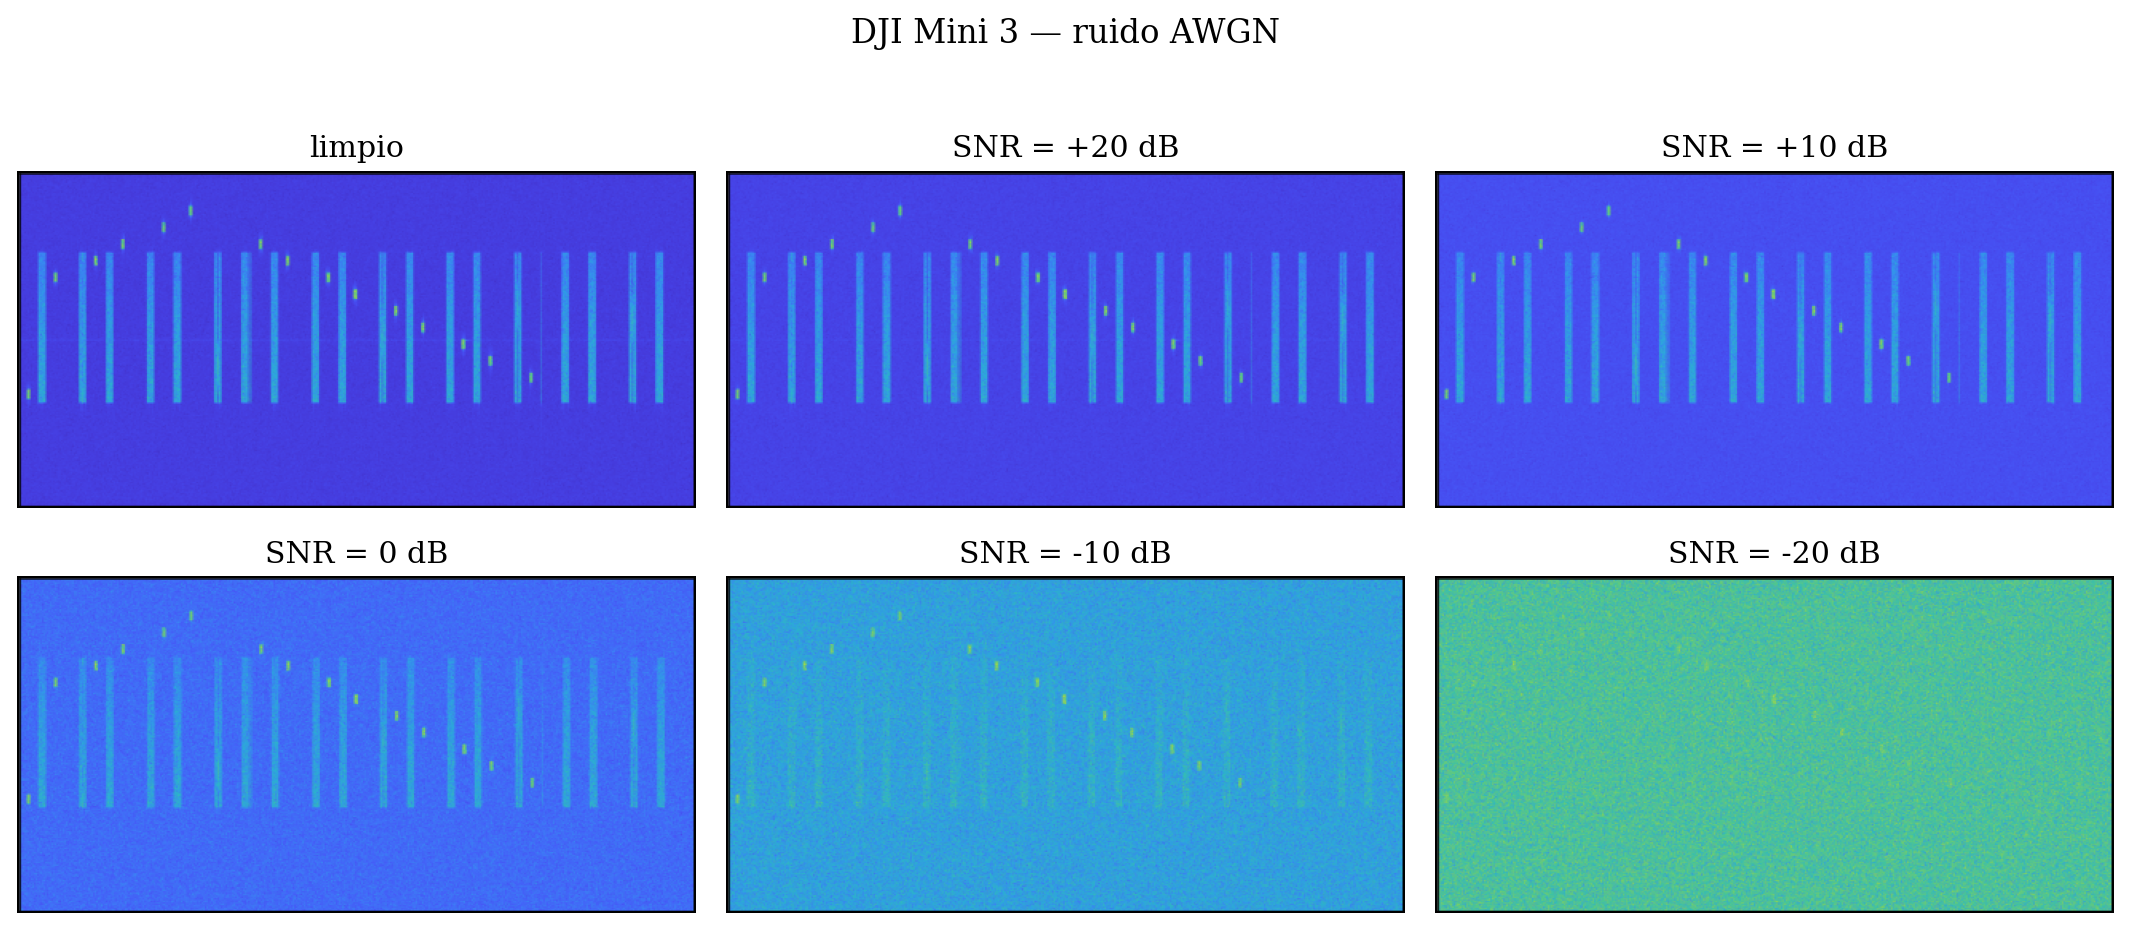
\includegraphics[width=\textwidth]{figuras/resultados/snr_ejemplo_mini3_awgn.png}
        \caption{Ruido AWGN: la energía se reparte por todo el plano. Al bajar el SNR, el fondo sube de forma uniforme hasta enmascarar por completo las ráfagas (a $-20$~dB la firma es inapreciable).}
        \label{fig:snr_ejemplo_awgn}
    \end{subfigure}

    \vspace{0.4em}

    \begin{subfigure}[b]{\textwidth}
        \centering
        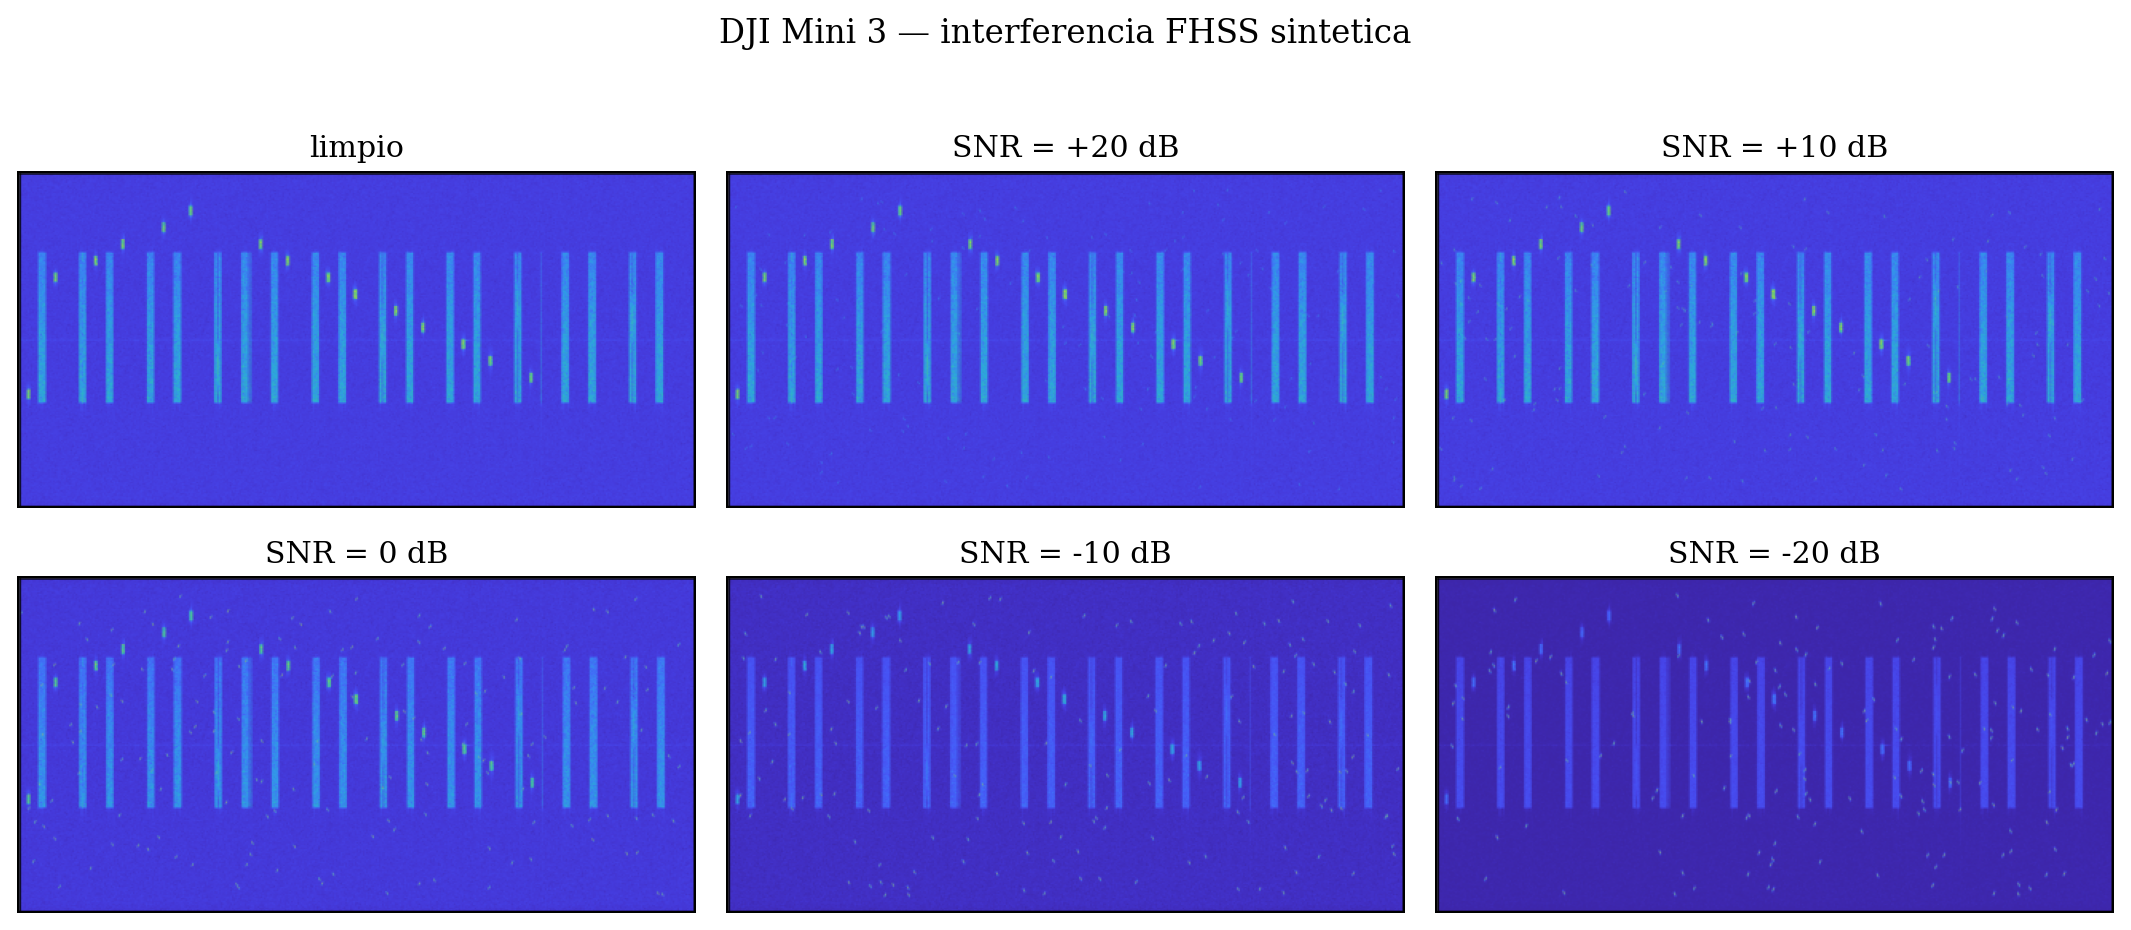
\includegraphics[width=\textwidth]{figuras/resultados/snr_ejemplo_mini3_fhss.png}
        \caption{Interferencia FHSS sintética: la energía se concentra en ráfagas puntuales. El fondo apenas cambia y las ráfagas de OcuSync del Mini~3 siguen siendo visibles incluso a SNR muy bajo.}
        \label{fig:snr_ejemplo_fhss}
    \end{subfigure}
    \caption{Efecto de los dos modelos de ruido sobre un espectrograma del DJI Mini~3 a distintos niveles de SNR, con la misma potencia total inyectada. El AWGN (a) destruye la firma espectral al subir el fondo de forma homogénea, mientras que el FHSS (b) deja intacto el \SI{98,5}{\percent} del plano tiempo-frecuencia y preserva la morfología de las ráfagas. Esta diferencia explica visualmente por qué el clasificador resiste mucho mejor el ruido FHSS.}
    \label{fig:snr_ejemplos}
\end{figure}



\begin{table}[htbp]
\centering
\caption{Exactitud del clasificador de seis clases frente al SNR para ruido AWGN e interferencia FHSS sintética.}
\label{tab:snr_accuracy}
\begin{tabular}{lcc}
\toprule
\textbf{SNR (dB)} & \textbf{AWGN} & \textbf{FHSS} \\
\midrule
$+\infty$ & 0,898 & 0,898 \\
$+20$     & 0,900 & 0,899 \\
$+10$     & 0,889 & 0,899 \\
$+5$      & 0,848 & 0,908 \\
$0$       & 0,691 & 0,912 \\
$-5$      & 0,239 & 0,852 \\
$-10$     & 0,136 & 0,748 \\
$-15$     & 0,133 & 0,676 \\
$-20$     & 0,133 & 0,557 \\
\bottomrule
\end{tabular}
\end{table}

La \cref{fig:snr_accuracy} representa gráficamente las dos curvas de exactitud frente al SNR.

\begin{figure}[htbp]
    \centering
    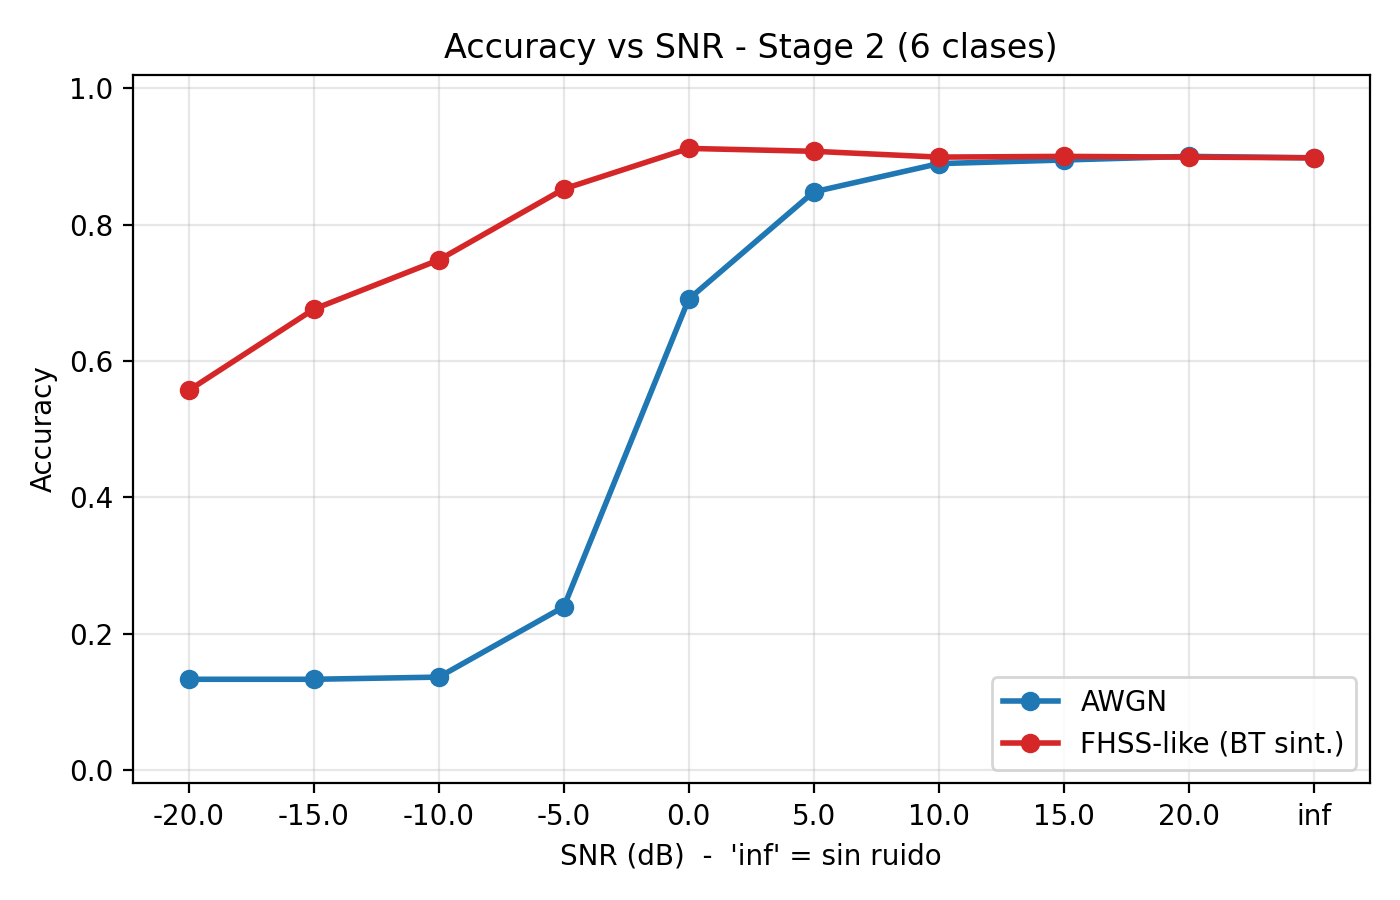
\includegraphics[width=0.85\textwidth]{figuras/resultados/snr_accuracy_vs_snr.png}
    \caption{Exactitud del clasificador frente al SNR para AWGN (azul) y FHSS sintético (naranja). El AWGN presenta un codo brusco entre $+5$~dB y $-5$~dB, con exactitud cayendo de \num{0,848} a \num{0,239}. El FHSS sintético mantiene exactitud superior a \num{0,85} hasta $-5$~dB y superior a \num{0,55} a $-20$~dB. La diferencia máxima entre ambas curvas, de \num{0,61}~puntos de exactitud, se alcanza a $-5$~dB.}
    \label{fig:snr_accuracy}
\end{figure}

La \cref{fig:snr_f1macro} muestra la evolución del macro-F1, que al tratar todas las clases por igual permite evaluar el impacto del ruido de forma independiente del desbalanceo entre clases.

\begin{figure}[htbp]
    \centering
    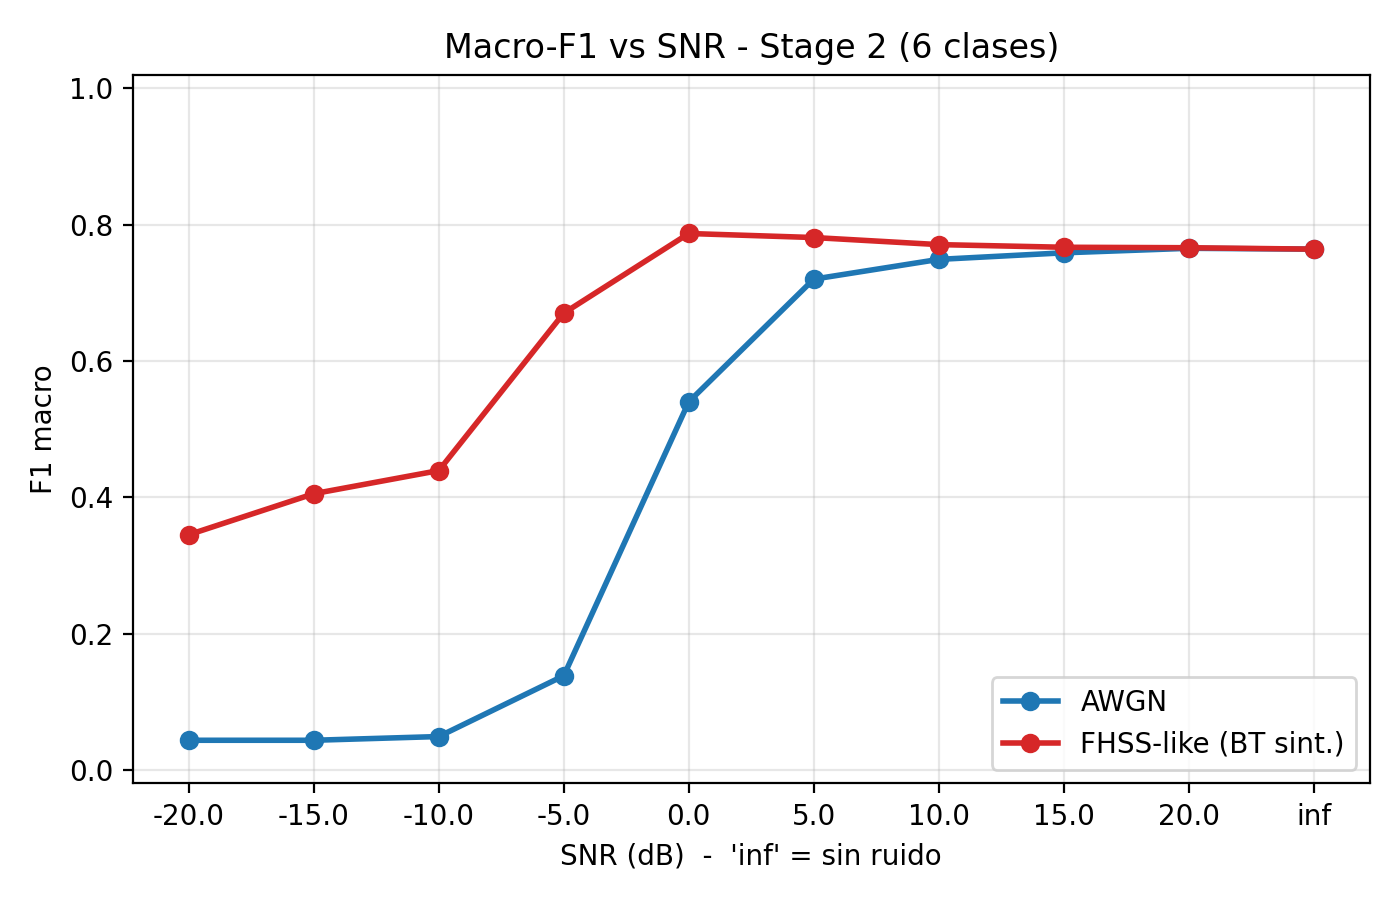
\includegraphics[width=0.85\textwidth]{figuras/resultados/snr_f1_macro_vs_snr.png}
    \caption{Macro-F1 del clasificador frente al SNR para ambos modelos de ruido. La tendencia es análoga a la de la exactitud: el AWGN produce una degradación notablemente más abrupta que el FHSS sintético.}
    \label{fig:snr_f1macro}
\end{figure}

La \cref{fig:snr_panel} muestra las matrices de confusión del clasificador a cuatro niveles de SNR representativos, para ambos modelos de ruido.

\begin{figure}[htbp]
    \centering
    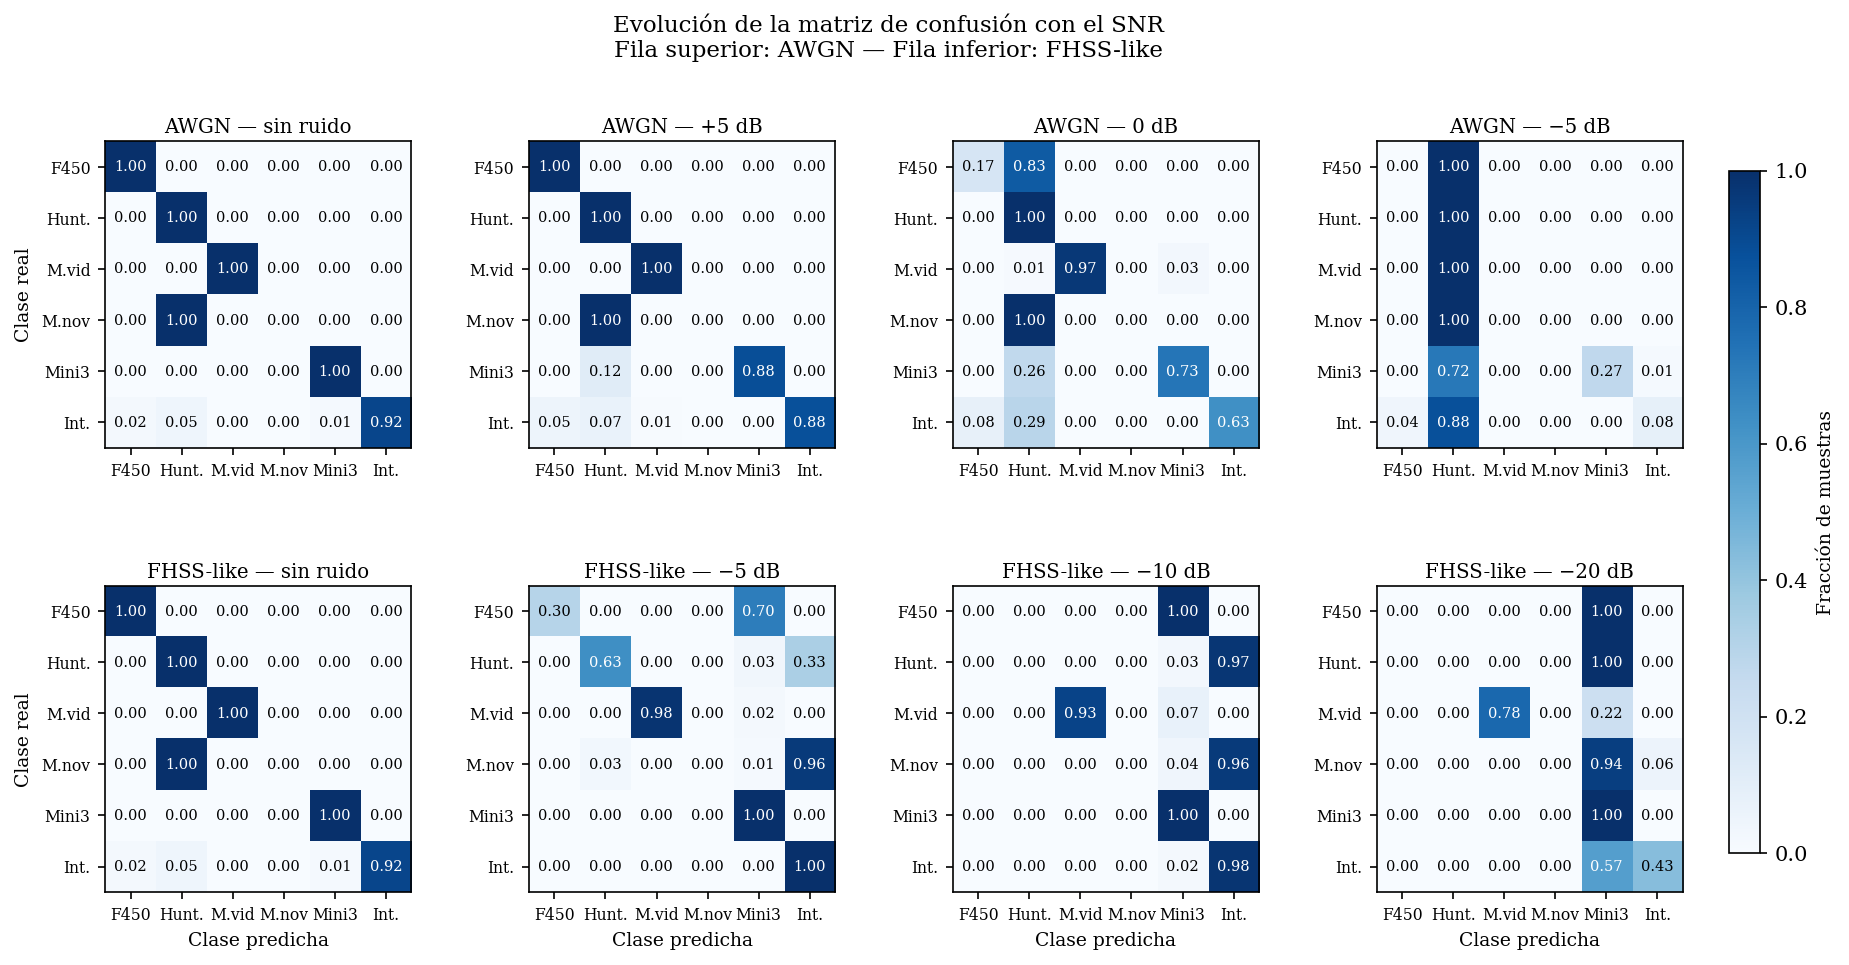
\includegraphics[width=\textwidth]{figuras/resultados/snr_confusion_panel.png}
    \caption{Panel de matrices de confusión del clasificador de seis clases a distintos niveles de SNR, para ruido AWGN (fila superior) y FHSS sintético (fila inferior). El AWGN dispersa las predicciones hacia clases incorrectas conforme decrece el SNR; el FHSS sintético mantiene la diagonal prácticamente intacta hasta $-5$~dB.}
    \label{fig:snr_panel}
\end{figure}

Las matrices del panel muestran que, bajo AWGN, la degradación es difusa: las predicciones se distribuyen hacia múltiples clases incorrectas conforme baja el SNR. Bajo FHSS sintético, en cambio, la diagonal se mantiene coherente hasta $-5$~dB y solo se degrada de forma apreciable a partir de $-10$~dB.

% =============================================================================
\subsection{Discusión}
\label{sec:p4_discusion}

\paragraph{Identificación del modelo de dron.}
La primera parte de P4 confirma que el sistema no solo detecta la presencia de un dron, sino que identifica su modelo concreto. El DJI Mini~3 ---la plataforma objetivo de este trabajo--- se clasifica correctamente en prácticamente la totalidad de las muestras (F1\,=\,\num{0,992}), y la clase \emph{interference} obtiene precisión \num{1,000}: ninguna señal real de interferencia se confunde de forma sistemática con un dron, en línea con la ausencia de confusión cruzada observada en P2 y P3. Los \num{25}~errores sobre \num{300}~muestras de interferencia se reparten entre varias clases de dron sin concentrarse en ninguna, lo que descarta un sesgo sistemático.

El único fallo relevante ---el colapso de \emph{mavic\_novideo} sobre \emph{hunter}--- no contradice la hipótesis central del trabajo, sino que la refuerza. Como muestra la \cref{fig:stage2_morfologia}, cuando el Mavic deja de transmitir vídeo su emisión se reduce a la señal de control FHSS, morfológicamente indistinguible de la del Hunter. Que el clasificador agrupe ambas clases es precisamente lo que cabe esperar de una red que decide por la \emph{forma} de la señal y no por una etiqueta o por el contexto de captura: ante dos morfologías idénticas, emite la misma predicción. El error no es, por tanto, un defecto del modelo, sino una limitación de los datos ---la ausencia, en ese modo de emisión, de cualquier rasgo espectral que separe las dos plataformas---, resoluble con más capturas de la clase en condiciones variadas y no con un rediseño del sistema.

\paragraph{Cómo se inyecta el ruido.}
Conviene recordar cómo se construyen ambos ruidos, descritos en detalle en la \cref{sec:implementacion_snr}, porque su forma de generación es la clave de la comparación. Los dos se inyectan en el dominio IQ complejo de la señal y se calibran a la \emph{misma potencia total} para cada SNR objetivo, de modo que la única variable que cambia entre ellos es cómo se reparte esa energía en el plano tiempo-frecuencia. 

El \textbf{ruido blanco AWGN} es ruido gaussiano complejo, $n[k]\sim\mathcal{CN}(0,\sigma^2)$, sumado muestra a muestra a la señal con la varianza $\sigma^2$ ajustada al SNR objetivo; al ser blanco, su energía se distribuye de forma uniforme por toda la banda y toda la ventana, elevando el fondo del espectrograma por igual en todo el plano. 

El \textbf{ruido FHSS sintético} emula una interferencia tipo Bluetooth Classic: genera unas \num{160}~ráfagas por ventana de \SI{0.1}{\second} (\num{1600}~saltos/s), cada una de \SI{366}{\micro\second} de duración y aproximadamente \SI{1}{\mega\hertz} de ancho, colocada en un instante y una frecuencia aleatorios dentro de la banda capturada y suavizada con una ventana de Hann. Como el conjunto se calibra a la misma potencia total que el AWGN, esa energía idéntica queda concentrada en rectángulos estrechos y dispersos ---morfológicamente parecidos a las propias ráfagas del dron--- que ocupan solo en torno al \SI{1,5}{\percent} del plano tiempo-frecuencia.

\paragraph{Robustez frente al ruido.}
La segunda parte de P4 somete al clasificador a dos modelos de ruido de la misma potencia total pero distinta distribución en el plano tiempo-frecuencia. El contraste es nítido tanto a nivel visual como cuantitativo. Visualmente (\cref{fig:snr_ejemplos}), el AWGN eleva el fondo de forma uniforme hasta enmascarar por completo las ráfagas a $-20$~dB, mientras que el FHSS sintético deja intacto el grueso del espectrograma y mantiene visibles las ráfagas de OcuSync incluso a SNR muy bajo. Cuantitativamente, esa diferencia se traduce en el codo abrupto del AWGN entre $+5$ y $-5$~dB ---una caída de \num{0,61}~puntos de exactitud--- frente a la degradación suave del FHSS, que conserva una exactitud superior a \num{0,85} hasta $-5$~dB.

Esta asimetría solo admite una explicación: la red discrimina por \emph{dónde} está la energía, no por \emph{cuánta} hay. El AWGN reparte su potencia por los \SI{40}{\mega\hertz} del espectrograma y, al superar el nivel de la señal, borra la firma de las ráfagas; el FHSS sintético concentra la misma potencia en aproximadamente el \SI{1,5}{\percent} del plano, de modo que el \SI{98,5}{\percent} restante ---y con él la morfología del dron--- permanece intacto. Si el clasificador se apoyase en el nivel medio de potencia, ambos ruidos lo degradarían por igual, dado que inyectan la misma energía total; que el AWGN sea mucho más destructivo demuestra lo contrario.

\paragraph{Síntesis: la red discrimina por morfología.}
Las dos partes de P4 convergen en la misma conclusión y cierran la hipótesis central del trabajo. La confusión \emph{mavic\_novideo}--\emph{hunter} muestra que la red agrupa señales por su morfología espectro-temporal; el barrido de SNR muestra que su decisión sobrevive mientras esa morfología sea visible y se desploma solo cuando el ruido la borra. Ambas observaciones son coherentes con los mapas de GradCAM del experimento P1 y de EigenCAM del experimento P2, donde las activaciones de la red se localizaban sobre las estructuras de ráfaga y no sobre el fondo. El clasificador no aprende la intensidad media de la captura ni un atajo contextual, sino la posición de la energía en el plano tiempo-frecuencia: la firma morfológica del dron. Este resultado, sólido para el DJI Mini~3 sobre el conjunto de prueba, sustenta la tesis del trabajo, con la cautela de que su validación en condiciones de despliegue más diversas queda planteada como línea futura.
% =============================================================================


\section{Detección de otros drones no vistos en el entrenamiento}
\label{sec:zeroshot}

Hasta aquí el detector se ha entrenado y evaluado únicamente con el DJI Mini~3. Surge entonces una pregunta natural: ¿lo que ha aprendido sirve para otros drones, o solo sabe reconocer al Mini~3? Para responderla se hace una prueba directa: se toma el detector ya entrenado, \emph{sin reentrenarlo ni ajustar nada}, y se le pasan espectrogramas de tres drones que nunca participaron en el entrenamiento ---un DJI~F450, un Mavic~Pro y un Hunter---, capturados al aire libre. Si el detector es capaz de localizar las ráfagas de estos drones desconocidos, será señal de que ha aprendido a reconocer la \emph{forma} de una transmisión FHSS en general, y no la firma concreta del Mini~3.

La distinción tiene una consecuencia práctica importante. Un lector de paquetes convencional necesitaría conocer y decodificar el protocolo de enlace de cada modelo de dron; en cambio, un detector que reconoce la forma de la señal funciona con cualquier dron que transmita de manera parecida, aunque emplee otro protocolo o una frecuencia distinta. Los tres drones de la prueba transmiten además en frecuencias centrales separadas entre \SI{30}{\mega\hertz} y \SI{50}{\mega\hertz} de la del entrenamiento, de modo que la prueba mide también si el detector depende de la posición absoluta en frecuencia.

\subsection{Cómo detecta las ráfagas de cada dron}
\label{sec:zeroshot_ejemplos}

La \cref{fig:zeroshot_comparativa} muestra la respuesta del detector ante un espectrograma representativo de cada plataforma. En el F450 y el Mavic~Pro el detector dibuja cajas rojas ---predicción \emph{drone}--- justo sobre las ráfagas FHSS, exactamente igual que hacía con el Mini~3, a pesar de no haberlos visto nunca durante el entrenamiento. En el Hunter, en cambio, no dibuja ninguna caja de dron.

\begin{figure}[htbp]
    \centering
    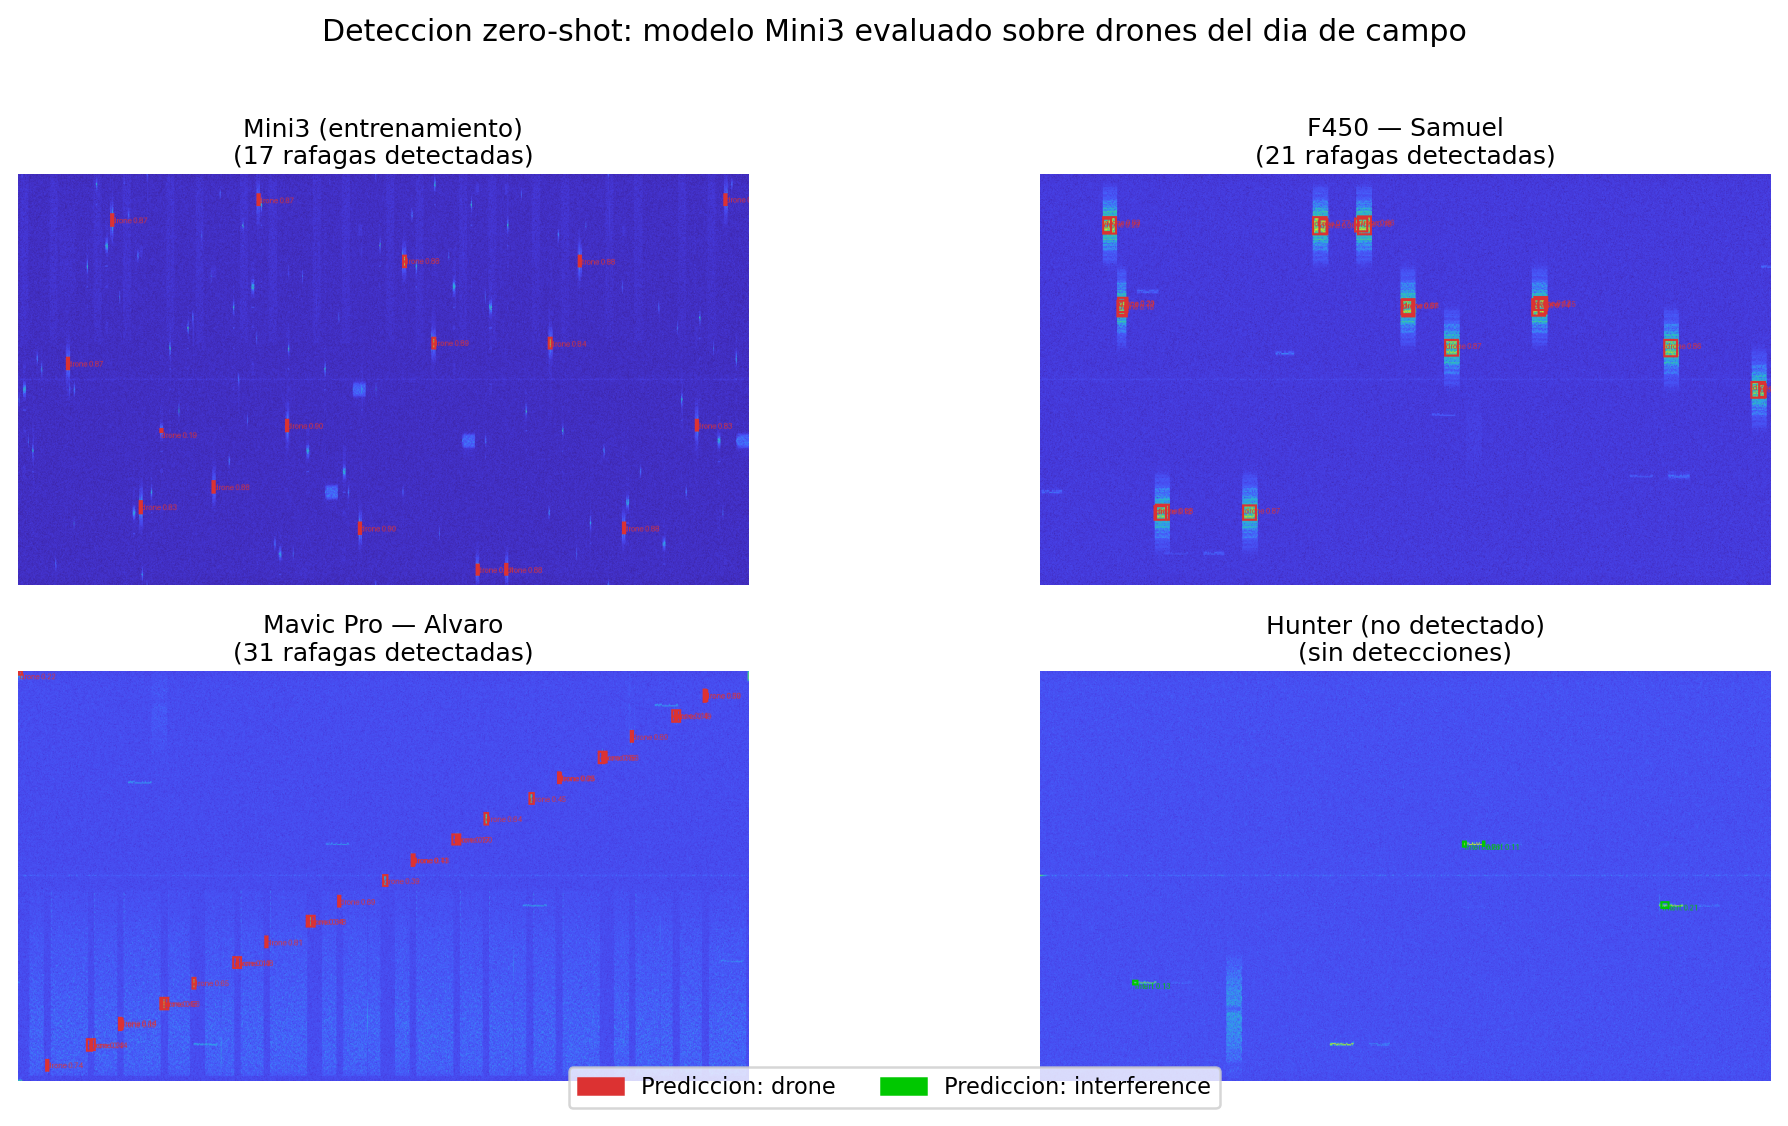
\includegraphics[width=\textwidth]{figuras/resultados/zeroshot_comparativa.png}
    \caption{Detección sobre drones no vistos en el entrenamiento. Para cada plataforma se muestra un espectrograma con las predicciones del detector superpuestas (rojo: \emph{drone}; verde: \emph{interference}). En el Mini~3 (referencia), el F450 y el Mavic~Pro el detector marca en rojo las ráfagas FHSS. En el Hunter no emite ninguna caja de dron, porque su señal no presenta esa morfología.}
    \label{fig:zeroshot_comparativa}
\end{figure}

\FloatBarrier
\subsection{Estadísticas: cuántas ráfagas detecta en cada dron}
\label{sec:zeroshot_estadisticas}

Para cuantificar el comportamiento basta con contar, de media, cuántas ráfagas de dron detecta en cada imagen y en qué porcentaje de imágenes confirma la presencia del dron (se declara presencia con al menos una ráfaga de dron detectada, con el mismo umbral de confianza $\mathit{thr}=0{,}10$ empleado en P3). La \cref{tab:zeroshot} resume el resultado sobre los más de \num{1800}~espectrogramas de los tres drones, y la \cref{fig:zeroshot_recall} lo representa gráficamente.

\begin{table}[htbp]
\centering
\caption{Resultado de la prueba de generalización sobre drones no vistos. La media de ráfagas es el número medio de cajas \emph{drone} por espectrograma; el recall de presencia es el porcentaje de imágenes en las que se confirma el dron.}
\label{tab:zeroshot}
\begin{tabular}{lcccc}
\toprule
\textbf{Dron} & \textbf{Protocolo} & \textbf{Imágenes} & \textbf{Ráfagas/imagen} & \textbf{Recall (\%)} \\
\midrule
DJI Mini~3 (ref.) & OcuSync~v2   & ---  & ---   & 99,0  \\
DJI F450          & OcuSync~v1   & 224  & 11,5  & 100,0 \\
Mavic~Pro         & OcuSync~v1   & 874  & 10,2  & 94,2  \\
Hunter            & Desconocido  & 788  & 0,0   & 0,5   \\
\bottomrule
\end{tabular}
\end{table}

\begin{figure}[htbp]
    \centering
    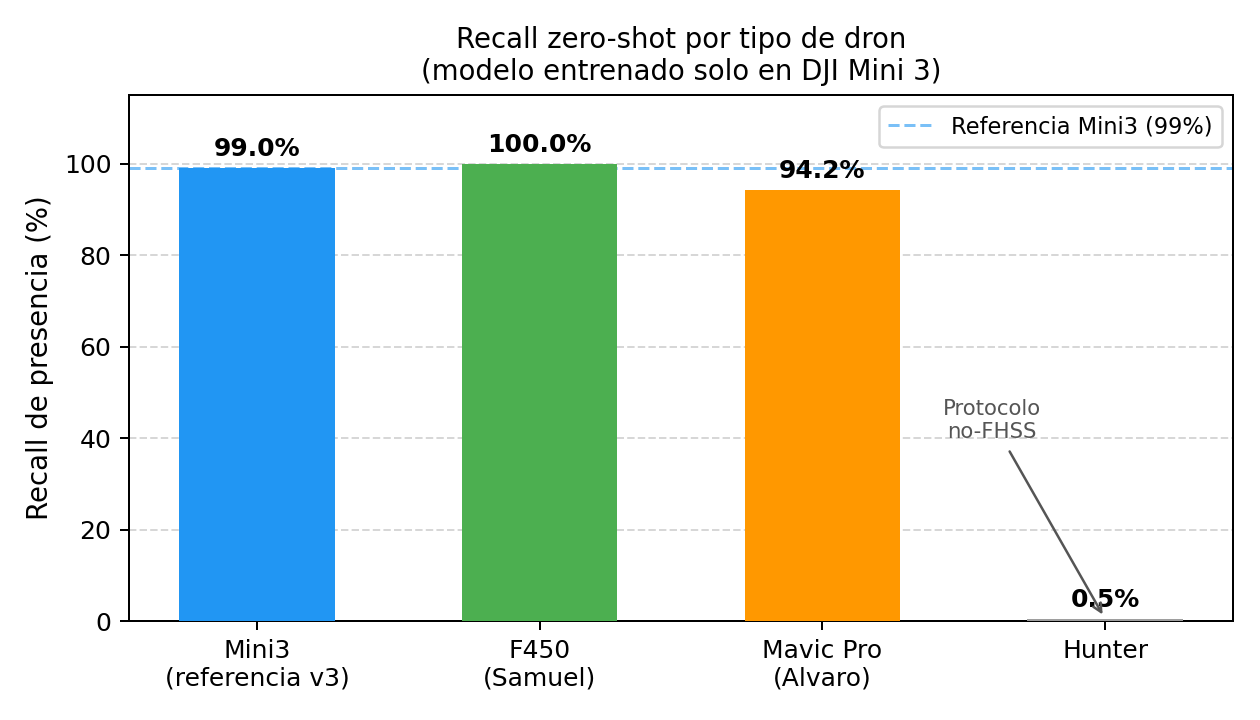
\includegraphics[width=0.8\textwidth]{figuras/resultados/zeroshot_recall_barras.png}
    \caption{Porcentaje de imágenes en las que el detector ---entrenado solo con el Mini~3--- confirma la presencia de dron, para cada plataforma. El F450 y el Mavic~Pro alcanzan el nivel de la referencia del Mini~3; el Hunter se queda en el \SI{0,5}{\percent} por no emitir señal FHSS.}
    \label{fig:zeroshot_recall}
\end{figure}

Los dos drones con protocolo OcuSync~v1 (F450 y Mavic~Pro) se comportan como el Mini~3: detecta en ellos una decena de ráfagas por imagen y confirma su presencia en casi todas las ventanas, sin reentrenamiento y pese a la diferencia de frecuencia. El Hunter, por el contrario, queda prácticamente sin detecciones de dron.

\FloatBarrier
\subsection{Por qué el detector no ve al Hunter}
\label{sec:zeroshot_hunter}

El fallo en el Hunter no es un error del detector, sino la consecuencia esperable de su criterio. El Hunter no transmite mediante saltos de frecuencia: su señal es de espectro ensanchado continuo (compatible con DSSS o un esquema propietario), sin las ráfagas compactas y separadas que caracterizan a OcuSync. Como el detector aprendió a buscar precisamente esa forma ---columnas cortas y aisladas en el plano tiempo-frecuencia--- y el Hunter no la presenta, no encuentra nada que marcar como dron.

Conviene subrayar un matiz: el detector no ignora la señal del Hunter, sino que la \emph{ve} y la clasifica como \emph{interference}. De hecho emite una media de \num{7,5}~cajas de interferencia por espectrograma, con al menos una en la totalidad de las \num{788}~imágenes. Es decir, reconoce que hay una señal activa, pero su morfología no es la de un salto FHSS, así que la asigna a la clase de interferencia y no a la de dron. El Hunter queda, por tanto, fuera del dominio para el que el sistema fue diseñado: el detector está pensado para señales FHSS, y el Hunter no lo es.

Este resultado, lejos de ser un punto débil, es la prueba más clara de qué ha aprendido el modelo. El detector reconoce la morfología FHSS allí donde aparece ---en drones distintos, con protocolos distintos y en frecuencias distintas--- y deja de detectar únicamente cuando esa morfología no existe. No ha memorizado al DJI~Mini~3: ha aprendido a reconocer la huella que deja un salto de frecuencia.

\subsection{Alcance del experimento: capturas de señal limpia}
\label{sec:zeroshot_alcance}

Conviene interpretar estas cifras tan altas en su justo contexto. Las capturas de campo de los tres drones se realizaron, en su mayoría, en condiciones de \emph{señal limpia}: con el dron como emisor dominante, a distancias moderadas y sin inyección de ruido ni interferencia intensa que solapara con sus ráfagas. Este experimento no pretende medir la robustez del detector frente al ruido ---esa cuestión se aborda por separado en el barrido de SNR del experimento P4---, sino responder a una pregunta más concreta: ¿reconoce el detector la morfología FHSS de un dron que nunca ha visto cuando esa morfología es claramente visible en el espectrograma? Para aislar esa pregunta es necesario, precisamente, partir de capturas en las que la firma del dron no esté enmascarada.

Por ello, los recall cercanos al \SI{100}{\percent} del F450 y el Mavic~Pro deben leerse como el rendimiento del detector en condiciones favorables, no como una garantía de comportamiento en cualquier escenario. En un despliegue real ---con interferencia WiFi y Bluetooth densa, mayores distancias, ángulos de antena desfavorables o niveles de señal más bajos--- es esperable que el recall descienda, igual que ocurría en el dataset~v3 del Mini~3 con las capturas más difíciles. El único indicio en esa dirección dentro de este experimento son las dos sesiones del Mavic~Pro con señal débil y las capturas con WiFi denso, donde el rendimiento ya muestra cierta sensibilidad a las condiciones de captura.

En resumen, lo que demuestra este experimento es la \emph{capacidad de transferencia} del detector a drones nuevos cuando la señal es observable, no su robustez en condiciones adversas. Ambas propiedades son necesarias para un sistema de vigilancia completo, pero se validan con experimentos distintos: la transferencia aquí, y la robustez frente al ruido en P4. La validación conjunta ---drones no vistos \emph{y} en condiciones de interferencia controlada--- requiere un conjunto de datos específico y queda planteada como trabajo futuro (dataset~v4).

\section{Discusión global}
\label{sec:discusion}

Las cuatro preguntas anteriores, junto con el experimento de detección de drones no vistos de la \cref{sec:zeroshot}, trazan una evolución metodológica coherente. La primera establece que la firma OcuSync es aprendible por un clasificador global en condición limpia, pero identifica los límites de esa formulación: ausencia de localización, incapacidad para representar clases coexistentes y riesgo de sesgo de contexto en escenarios de despliegue más generales. La segunda demuestra que un detector de objetos supera esas limitaciones localizando morfológicamente las ráfagas con cero confusión cruzada, al precio de un recall de caja moderado que se explica por el etiquetado automático débil y la ligereza del modelo. La tercera muestra que ese recall moderado no impide una vigilancia operativa fiable: agregando varias detecciones por ventana temporal se alcanza el \SI{91}{\percent} de recall de presencia con precisión y especificidad perfectas. La cuarta cierra el argumento con dos resultados complementarios: el clasificador de modelos identifica el DJI Mini~3 sin errores, y el barrido de robustez demuestra cuantitativamente que la discriminación se basa en la morfología y no en la intensidad. Este experimento confirma esa hipótesis desde fuera del conjunto de entrenamiento: el detector generaliza a OcuSync~v1 (F450 y Mavic~Pro) sin reentrenamiento, clasifica activamente la señal del Hunter como interferencia ---demostrando que ve la señal pero distingue su morfología de la FHSS--- y mantiene robustez frente a cambios de frecuencia central de hasta \SI{50}{\mega\hertz}.

El principal resultado positivo del sistema es la ausencia de falsos positivos en todas las condiciones evaluadas: cuando el detector afirma que una ráfaga es de dron, no se equivoca de clase; y cuando el clasificador de presencia confirma que hay un dron en la escena, no se equivoca de imagen. La principal limitación es el recall a nivel de caja, consecuencia del etiquetado automático ruidoso, el reducido tamaño de las ráfagas tras el redimensionado y el uso de un modelo ligero. El análisis de presencia demuestra que esta limitación es tolerable en condición operativa; sin embargo, mejorar el etiquetado ---ya sea con datos adicionales o con anotación manual parcial de las ráfagas más débiles--- es la vía más directa para aumentar la sensibilidad del sistema.

Operativamente, el sesgo del sistema hacia falsos negativos (no detectar una ráfaga individual) es preferible al sesgo hacia falsos positivos (confirmar presencia de dron en una escena sin dron), especialmente en un contexto de primera alerta donde una alarma espuria tiene coste operativo. El sistema en dos etapas se comporta como una primera versión sólida de vigilancia RF, cuyo margen de mejora reside en la cobertura de ráfagas individuales y no en la separabilidad entre clases.

% =============================================================================
% Capitulo 6 - Conclusiones y lineas futuras
% =============================================================================
\chapter{Conclusiones y líneas futuras}
\label{cap:conclusiones}

\section{Conclusiones}
\label{sec:conclusiones}

Este Trabajo Fin de Grado ha evolucionado desde un enfoque inicial de clasificación global de espectrogramas hacia una arquitectura más robusta de detección e identificación en dos etapas. La primera etapa, basada en YOLOv8, localiza ráfagas en el espectrograma y las clasifica como \emph{drone} o \emph{interference}. La segunda etapa, basada en clasificadores como ResNet18, se reserva para la identificación de modelos de dron una vez detectada la presencia de señal compatible con UAV.

La principal conclusión experimental es que la firma tiempo-frecuencia del DJI Mini 3 es separable morfológicamente de las interferencias consideradas en la banda de \SI{2.4}{\giga\hertz}. El detector YOLOv8n entrenado durante 60 épocas alcanza en test una precisión global de 0,760, un recall global de 0,391, un mAP@50 de 0,388 y un mAP@50-95 de 0,203. Aunque el recall es limitado, la matriz de confusión normalizada no muestra confusión cruzada entre las clases activas \emph{drone} e \emph{interference}. Esto significa que, cuando el modelo emite una detección positiva, distingue correctamente la morfología de ambas clases.

El cambio metodológico resulta relevante. El baseline de clasificación global podía aprender sesgos contextuales de la captura, mientras que YOLO obliga al modelo a aprender regiones locales de señal. Esto hace que el resultado sea más interpretable y más coherente con el fenómeno físico que se desea detectar: ráfagas FHSS/OcuSync en el dominio tiempo-frecuencia.

\section{Limitaciones}
\label{sec:limitaciones}

La primera limitación es el recall del detector. El modelo no detecta todos los bursts anotados, por lo que todavía no puede considerarse un contador exhaustivo de ráfagas. Esta limitación puede deberse al pequeño tamaño de muchas regiones, al redimensionamiento de la imagen a \num{640}x\num{640}, al uso de YOLOv8n como arquitectura ligera y al carácter automático de las etiquetas.

La segunda limitación es el etiquetado débil. Las cajas se generan mediante umbrales y filtros morfológicos, no mediante anotación manual. Aunque este procedimiento es coherente y reproducible, puede producir etiquetas incompletas o inconsistentes en casos frontera. Una validación manual de un subconjunto permitiría estimar mejor la calidad del \emph{ground truth}.

La tercera limitación es la heterogeneidad de la clase \emph{interference}. Esta clase agrupa Bluetooth, WiFi residual y ruido, por lo que resulta más difícil de modelar que la clase \emph{drone}, asociada a una firma más homogénea del DJI Mini 3.

\section{Líneas futuras}
\label{sec:lineas_futuras}

Como trabajo futuro inmediato se propone entrenar variantes de mayor capacidad, como YOLOv8s o YOLOv8m, para comprobar si aumenta el recall sin introducir confusión entre clases activas. También sería conveniente realizar una anotación manual parcial de espectrogramas para validar el auto-etiquetado y medir cuánto afecta el ruido de etiquetas al rendimiento.

Otra línea directa es completar la segunda etapa de identificación de modelos de dron. Para ello se pueden utilizar capturas de distintos UAV, generar espectrogramas o recortes a partir de las regiones detectadas, y entrenar un clasificador multiclase como ResNet18. Esta etapa permitiría pasar de un sistema de detección de presencia a un sistema de detección e identificación.

Finalmente, el sistema puede extenderse hacia una versión operativa de búsqueda y confirmación. En dicha versión, GNU Radio barrería frecuencias de interés, Python generaría espectrogramas cortos y YOLO decidiría si bloquear la frecuencia para realizar una captura más larga. Este esquema conectaría el detector offline desarrollado en el TFG con un demostrador práctico de vigilancia RF.


% =============================================================================
% Anexos
% =============================================================================
\appendix
% =============================================================================
% Capitulo 7 - Anexos
% =============================================================================
\chapter{Material complementario}
\label{cap:anexos}

\section{Acrónimos}
\label{anexo:acronimos}

\begin{acronym}[SigMF]
  \acro{TFG}{Trabajo Fin de Grado}
  \acro{UAV}{vehículo aéreo no tripulado (\emph{Unmanned Aerial Vehicle})}
  \acro{UAS}{sistema aéreo no tripulado (\emph{Unmanned Aircraft System})}
  \acro{DJI}{\emph{Da-Jiang Innovations}}
  \acro{RF}{radiofrecuencia}
  \acro{SDR}{radio definida por software (\emph{Software Defined Radio})}
  \acro{IQ}{componentes en fase y cuadratura}
  \acro{ISM}{banda industrial, científica y médica (\emph{Industrial, Scientific and Medical})}
  \acro{USRP}{\emph{Universal Software Radio Peripheral}}
  \acro{SigMF}{\emph{Signal Metadata Format}}
  \acro{STFT}{transformada de Fourier de tiempo corto (\emph{Short-Time Fourier Transform})}
  \acro{FFT}{transformada rápida de Fourier (\emph{Fast Fourier Transform})}
  \acro{FHSS}{salto de frecuencia (\emph{Frequency Hopping Spread Spectrum})}
  \acro{DSSS}{espectro ensanchado por secuencia directa (\emph{Direct Sequence Spread Spectrum})}
  \acro{OFDM}{multiplexación por división de frecuencias ortogonales (\emph{Orthogonal Frequency Division Multiplexing})}
  \acro{AFH}{salto de frecuencia adaptativo (\emph{Adaptive Frequency Hopping})}
  \acro{GFSK}{modulación por desplazamiento de frecuencia gaussiana (\emph{Gaussian Frequency Shift Keying})}
  \acro{AWGN}{ruido blanco gaussiano aditivo (\emph{Additive White Gaussian Noise})}
  \acro{SNR}{relación señal a ruido (\emph{Signal-to-Noise Ratio})}
  \acro{AGC}{control automático de ganancia (\emph{Automatic Gain Control})}
  \acro{CNN}{red neuronal convolucional (\emph{Convolutional Neural Network})}
  \acro{ResNet}{red residual (\emph{Residual Network})}
  \acro{PCA}{análisis de componentes principales (\emph{Principal Component Analysis})}
  \acro{YOLO}{\emph{You Only Look Once}}
  \acro{mAP}{precisión media promediada (\emph{mean Average Precision})}
  \acro{IoU}{intersección sobre la unión (\emph{Intersection over Union})}
  \acro{COCO}{\emph{Common Objects in Context}}
  \acro{GNSS}{sistema global de navegación por satélite (\emph{Global Navigation Satellite System})}
  \acro{NLOS}{sin línea de visión directa (\emph{Non Line of Sight})}
  \acro{RCS}{sección radar (\emph{Radar Cross Section})}
  \acro{GPU}{unidad de procesamiento gráfico (\emph{Graphics Processing Unit})}
\end{acronym}

\section{Convención de nombres de captura}
\label{anexo:nombres}

Para mantener trazabilidad se recomienda utilizar nombres de captura con campos explícitos:

\begin{lstlisting}[caption={Formato recomendado de nombre de captura.}]
<dron>_<label>_<distancia/nodrone>_<wifi_level>_<sesion>_<capNN>
\end{lstlisting}

Ejemplos:

\begin{lstlisting}[caption={Ejemplos de nombres de captura.}]
mini3_drone_d5_w1_s01_cap01
mini3_drone_d10_w3_s02_cap01
mini3_nodrone_w1_s01_cap03
mini3_nodrone_w3_s01_cap03
\end{lstlisting}

En el CSV de entrenamiento, la etiqueta de captura debe normalizarse como \texttt{drone} o \texttt{interference}, aunque el nombre mantenga el prefijo \texttt{nodrone} para indicar que el dron estaba apagado.

\section{Composición detallada del dataset v3}
\label{anexo:dataset_v3}

La \cref{tab:anexo_dataset_v3} detalla las \num{21}~capturas del dataset~v3 (\num{150}~espectrogramas cada una, \num{3150} en total), con su distancia, nivel de WiFi, frecuencia central y partición. El prefijo \texttt{mini3\_} se omite por brevedad. La partición se realiza por captura completa para evitar fuga de información entre entrenamiento, validación y prueba.

\begin{table}[htbp]
\centering
\footnotesize
\caption{Composición del dataset v3 por captura.}
\label{tab:anexo_dataset_v3}
\begin{tabular}{lccccc}
\toprule
\textbf{Captura} & \textbf{Clase} & \textbf{Dist. (m)} & \textbf{WiFi} & \textbf{$f_c$ (MHz)} & \textbf{Partición} \\
\midrule
drone\_d10\_w1\_s01\_cap01 & drone & 10 & 1 & 2450 & train \\
drone\_d10\_w1\_s01\_cap02 & drone & 10 & 1 & 2450 & train \\
drone\_d10\_w2\_s02\_cap01 & drone & 10 & 2 & 2460 & train \\
drone\_d10\_w2\_s02\_cap02 & drone & 10 & 2 & 2470 & val \\
drone\_d10\_w3\_s02\_cap01 & drone & 10 & 3 & 2460 & test \\
drone\_d10\_w3\_s02\_cap02 & drone & 10 & 3 & 2470 & train \\
drone\_d5\_w1\_s01\_cap01  & drone & 5  & 1 & 2450 & test \\
drone\_d5\_w1\_s01\_cap02  & drone & 5  & 1 & 2470 & val \\
drone\_d5\_w2\_s02\_cap01  & drone & 5  & 2 & 2450 & train \\
drone\_d5\_w2\_s02\_cap02  & drone & 5  & 2 & 2475 & train \\
drone\_d5\_w3\_s02\_cap01  & drone & 5  & 3 & 2450 & train \\
drone\_d5\_w3\_s02\_cap02  & drone & 5  & 3 & 2470 & train \\
nodrone\_w1\_s01\_cap01 & interference & n/a & 1 & 2422 & train \\
nodrone\_w1\_s01\_cap02 & interference & n/a & 1 & 2422 & train \\
nodrone\_w1\_s01\_cap03 & interference & n/a & 1 & 2422 & test \\
nodrone\_w2\_s01\_cap01 & interference & n/a & 2 & 2422 & train \\
nodrone\_w2\_s01\_cap02 & interference & n/a & 2 & 2422 & train \\
nodrone\_w2\_s01\_cap03 & interference & n/a & 2 & 2422 & train \\
nodrone\_w3\_s01\_cap01 & interference & n/a & 3 & 2422 & train \\
nodrone\_w3\_s01\_cap02 & interference & n/a & 3 & 2422 & val \\
nodrone\_w3\_s01\_cap03 & interference & n/a & 3 & 2422 & test \\
\midrule
\multicolumn{6}{l}{\textbf{Total:} train \num{2100} (14 capturas), val \num{450} (3 capturas), test \num{600} (4 capturas)} \\
\bottomrule
\end{tabular}
\end{table}

Las capturas de dron se registraron en frecuencias centrales de \SIrange{2450}{2475}{\mega\hertz} y las de interferencia a \SI{2422}{\mega\hertz}. Esta diferencia de portadora entre clases no afecta a la decisión del detector, que opera sobre la morfología local de las ráfagas tras la normalización frecuencial (\texttt{FrequencyNormalize}), pero se documenta aquí por transparencia; su eliminación mediante portadoras espejadas entre clases se contempla en el dataset~v4 propuesto en el \cref{cap:conclusiones}.

\section{Configuración de entrenamiento de los modelos}
\label{anexo:hiperparametros}

La \cref{tab:anexo_hiperparametros} resume la configuración de los tres modelos entrenados en el trabajo: el detector YOLOv8n de la primera etapa, el clasificador ResNet18 de seis clases de la segunda etapa y el clasificador binario ResNet18 del experimento P1.

\begin{table}[htbp]
\centering
\footnotesize
\caption{Hiperparámetros de los tres modelos entrenados.}
\label{tab:anexo_hiperparametros}
\begin{tabular}{lll}
\toprule
\textbf{YOLOv8n (Stage 1)} & \textbf{ResNet18 (Stage 2)} & \textbf{ResNet18 binario (P1)} \\
\midrule
Base: yolov8n.pt (COCO)      & Base: ResNet18 (ImageNet)   & Base: ResNet18 (ImageNet) \\
Entrada: 640$\times$640       & Entrada: 224$\times$224     & Entrada: 224$\times$224 \\
Lote: 16                      & Lote: 32                    & Lote: 32 \\
Épocas: 60 (baseline 15)      & Épocas: 30 (mejor en la 10) & Épocas: 20 (mejor en la 5) \\
Optimizador: SGD              & Optimizador: AdamW          & Optimizador: AdamW \\
Semilla: 42                   & lr $10^{-4}$, wd $10^{-4}$   & lr $10^{-4}$, wd $10^{-4}$ \\
Aumentos geom. desactivados   & CosineAnnealingLR           & CosineAnnealingLR \\
(fliplr, flipud, degrees,     & 3 grupos congelados         & 3 capas congeladas \\
shear, perspective = 0)       & FrequencyNormalize          & FrequencyNormalize \\
                              & Semilla: 42                 & Semilla: 42 \\
\bottomrule
\end{tabular}
\end{table}

\section{Parámetros del barrido de SNR}
\label{anexo:snr_params}

El barrido evalúa el clasificador de seis clases (\num{941}~segmentos de prueba) inyectando ruido en el dominio IQ a los niveles de SNR $\{+\infty,\, +20,\, +15,\, +10,\, +5,\, 0,\, -5,\, -10,\, -15,\, -20\}$~dB, regenerando el espectrograma con el mismo \emph{pipeline} de entrenamiento (STFT con ventana de Hann de \num{1024}~muestras, solape \SI{75}{\percent}, mapa de color parula, \num{1024}$\times$\num{576}~píxeles). Se comparan dos modelos de ruido calibrados a la misma potencia total:

\begin{itemize}
  \item \textbf{AWGN:} ruido gaussiano complejo $n[k]\sim\mathcal{CN}(0,\sigma^2)$, con $\sigma^2$ ajustada al SNR objetivo, distribuido uniformemente por todo el plano tiempo-frecuencia.
  \item \textbf{FHSS sintético:} \num{160}~ráfagas por ventana de \SI{0.1}{\second} (\num{1600}~saltos/s), cada una de \SI{366}{\micro\second} de duración y aproximadamente \SI{1}{\mega\hertz} de ancho, situadas en frecuencia e instante aleatorios dentro del \SI{90}{\percent} de la banda capturada, con modulación GFSK simplificada (chirp de $\pm$\SI{250}{\kilo\hertz}) y ventana de Hann en amplitud.
\end{itemize}

\section{Pseudocódigo del auto-etiquetado YOLO}
\label{anexo:pseudocodigo_autolabel}

\begin{lstlisting}[style=python,caption={Pseudocódigo de generación automática de cajas YOLO.}]
for image_path in spectrograms:
    img = read_image(image_path)
    intensity = rgb_to_intensity(img)
    threshold = percentile(intensity, 99.8)
    mask = intensity > threshold
    components = connected_components(mask)

    for comp in components:
        box = bounding_box(comp)
        area = box.width * box.height

        if area < 8:
            continue
        if area > 0.005 * image_width * image_height:
            continue

        class_id = class_from_capture_name(image_path)
        write_yolo_box(image_path, class_id, box)
\end{lstlisting}

\section{Pseudocódigo del detector YOLO}
\label{anexo:pseudocodigo_detector_yolo}

\begin{lstlisting}[style=python,caption={Pseudocódigo de inferencia del detector YOLO.}]
iq = read_iq_window(capture, duration=0.1)
spectrogram = make_spectrogram(iq)
detections = yolo.predict(spectrogram)

for det in detections:
    if det.confidence < threshold:
        continue
    if det.class_name == "drone":
        alert = True
        crop = crop_region(spectrogram, det.box)
\end{lstlisting}

\section{Pseudocódigo de búsqueda y confirmación}
\label{anexo:pseudocodigo_busqueda}

Una versión operativa del sistema podría recorrer varias frecuencias, generar espectrogramas cortos y bloquear la frecuencia cuando el detector confirme presencia de dron:

\begin{lstlisting}[style=python,caption={Pseudocódigo de búsqueda y confirmación con YOLO.}]
centers = [2.410e9, 2.425e9, 2.440e9, 2.455e9, 2.470e9, 2.485e9]

for fc in centers:
    tune_usrp(fc)
    iq = capture_short(duration=0.25)
    spec = make_spectrogram(iq)
    detections = yolo.predict(spec)

    if has_drone_detection(detections, conf=0.80):
        iq2 = capture_short(duration=0.25)
        spec2 = make_spectrogram(iq2)
        detections2 = yolo.predict(spec2)

        if has_drone_detection(detections2, conf=0.80):
            lock_frequency(fc)
            capture_long(duration=3.0)
            break
\end{lstlisting}

\section{Pseudocódigo de identificación de modelos}
\label{anexo:pseudocodigo_modelos}

\begin{lstlisting}[style=python,caption={Pseudocódigo de clasificación multiclase como segunda etapa.}]
spec = make_spectrogram(iq_window)
detections = yolo.predict(spec)

for det in detections:
    if det.class_name != "drone":
        continue
    crop = crop_region(spec, det.box)
    probs = model_multiclass.predict(crop)
    model_id = argmax(probs)
    confidence = max(probs)
\end{lstlisting}

\section{Disponibilidad de código, modelos y datos}
\label{anexo:disponibilidad}

El código de adquisición, generación de espectrogramas, auto-etiquetado, entrenamiento y evaluación, la fuente \LaTeX{} de esta memoria y los resultados consolidados (métricas y figuras) están disponibles en el repositorio del proyecto: \url{https://github.com/edumateoss/spectre-main}. Los \emph{datasets} de espectrogramas, las capturas IQ en formato SigMF y los pesos de los modelos entrenados (detector YOLOv8n y clasificador ResNet18) no se incluyen en el repositorio por su tamaño y se entregan como ficheros asociados a esta memoria. La estructura del repositorio, los comandos de reproducción y las versiones de las dependencias se documentan en el fichero \texttt{README} incluido.


% =============================================================================
% Bibliografia
% =============================================================================
\backmatter

\printbibliography[heading=bibintoc,title={Bibliografía}]

\end{document}
